%%%%%%%%%%%%%%%%%%%%%%%%%%%%%%%%%%%%%%%%%%%%%%%%%%%%%%%%%%%%%%%%%%%%%%%%%%%%%%%%%%%%%%%%%%%%%%%
%%                                  Thesis Main Document                                     %%
%%%%%%%%%%%%%%%%%%%%%%%%%%%%%%%%%%%%%%%%%%%%%%%%%%%%%%%%%%%%%%%%%%%%%%%%%%%%%%%%%%%%%%%%%%%%%%%
\documentclass{thesisclass}
% as defined in thesisclass.cls

% ----------------------------------------------------------------------------------------------
%|                                  General Information                                         |
% ----------------------------------------------------------------------------------------------
% ---------------------------------------------------------------
%|                    Infos about thesis                         |
% ---------------------------------------------------------------
\newcommand{\myname}{Gunnar Diestmann}
\newcommand{\mytitle}{Trajektorienplanung f\"ur einen kooperativen Fahrstreifenwechsel hochautomatisierter
                      Fahrzeuge}

\newcommand{\reviewerone}{Prof. Dr.-Ing. Christoph Stiller}
\newcommand{\advisor}{Maximilian Naumann, M.Sc.}

\newcommand{\timeandplace}{Karlsruhe, Mai 2019}

\newcommand{\frontmatterhint}{Draft! / Vorl\"aufige Fassung!}

% ---------------------------------------------------------------
%|                    Infos for PDF file                         |
% ---------------------------------------------------------------
\hypersetup{
 pdfauthor={\myname},
 pdftitle={\mytitle},
 pdfsubject={Thesis},
 pdfkeywords={Trajektorienplanung, kooperative Verhaltensplanung, Multi-Agenten-Optimimierung, Fahrstreifenwechsel,
              Kostenfunktional, Pfadplanung}
}

%\usepackage[english]{babel}  	% English
\usepackage[ngerman]{babel}  	% German
\usepackage[ngerman]{translator} 


% ----------------------------------------------------------------------------------------------
%|                                My packages/commands                                          |
% ----------------------------------------------------------------------------------------------
% track changes
    %\usepackage{changes} 		% highlight changes
	\usepackage[final]{changes}	% don't highlight changes

% tables
	\usepackage{array,multirow,graphicx}

% pseudocode
	\usepackage[ruled,vlined]{algorithm2e}

% for forcing positions of tables, figures, ...
	\usepackage{float}

% units
	\usepackage{siunitx}
	\usepackage{dcolumn}


% ----------------------------------------------------------------------------------------------
%|                                       Glossaries                                             |
% ----------------------------------------------------------------------------------------------
% In order to make use glossaries work:
% 	* the latex installation folder musst be added to `$PATH`
%	* perl must be installed and added to `$PATH`
%	* Document Build: pdflatex thesis / makeglosseries thesis / pdflatex thesis / pdflatex thesis
% Adding something to `$PATH`:
% Windows: 	1. Copie path to latex installation folder
%			2. Search for "Umgebunsvariablen für dieses Konto bearbeiten"
%			3. Path -> Bearbeiten -> paste in path to latex installation folder (\bin)
%			4. Test in command-line with where <programm_name> (e.g. where latex/ where perl)
% Linux:  ToDo
% Mac:    ToDo
\newif\ifuseglossaries			% as the glossaries package sometimes causes problems, you can switch if of
								% if switching of, remember to remove all \gls{}/... statements
								
\useglossariestrue				% use glossaries (acronyms and online references)
% \useglossariesfalse			% don't use glossaries

\ifuseglossaries
	\usepackage[acronym,xindy,toc,nomain,nonumberlist,nopostdot,notranslate]{glossaries}%

	%% Create new glosseries	
	%Online Referenzen Verzeichnis hinzufügen	
	\newglossary[onlineref]{onlineref}{onli}{onlo}{Online Referenzen}
	
	%Ein eigenes Symbolverzeichnis erstellen
	\newglossary[slg]{symbolslist}{syi}{syg}{Symbolverzeichnis}
 
	%Den Punkt am Ende jeder Beschreibung deaktivieren
	\renewcommand*{\glspostdescription}{}
	
	%% Create new styles for glosseries
	% mylong used for Symbolverzeichnis
	\newglossarystyle{mylong}{%
  		\setglossarystyle{long}%
  		\renewcommand*{\glsnamefont}[1]{\textbf{##1}}%
  	}%
  	% mylist used for Online Refernzen
  	\newglossarystyle{mylist}{%
  		\setglossarystyle{list}%
  		\renewcommand*{\glsnamefont}[1]{\textrm{\textmd{##1}}}%
  	}%
  	
  	\makeglossaries
  	
	% ordinary acronyms
	\newacronym{idm}{IDM}{Inteligent Driver Model}
\newacronym{mcts}{MCTS}{Monte Carlo Tree Search}
\newacronym{ettc}{ETTC}{Enhanced Time to Collision}
\newacronym{pvd}{PVD}{Path Velocity Decomposition}
\newacronym{ros}{ROS}{Robot Operating System} 
	
	% symbols	
	% usage: \gls{} \glspl{} or \acrshort{}
	
%Befehle für Symbole
%Zeit
\newglossaryentry{symb:t_lc}{
name=$t_\mathrm{lc}$,
description={Zeitpunkt des Fahrstreifenwechsels: Fahrbahnmarkierung wird \"uberquert [$s$]},
sort=atimelanechange, type=symbolslist
}
\newglossaryentry{symb:t_coop,start}{
name=$t_\mathrm{coop,start}$,
description={Beginn der Kooperation [$s$]},
sort=atimecoopstart, type=symbolslist
}
\newglossaryentry{symb:t_coop,end}{
name=$t_\mathrm{coop,end}$,
description={Ende der Kooperation [$s$]},
sort=atimecoopend, type=symbolslist
}
\newglossaryentry{symb:t_abs}{
name=$T_\mathrm{abs}$,
description={Gew\"unschter Zeitabstand zum vorausfahrenden Fahrzeug [$s$]},
sort=atimeabs, type=symbolslist
}
\newglossaryentry{symb:t_lcd}{
name=$t_\mathrm{lcd}$,
description={Dauer des Fahrstreifenwechsels [$s$]},
sort=atimelanechangedauer, type=symbolslist
}
\newglossaryentry{symb:t_verarb}{
name=$t_\mathrm{verarb}$,
description={Ben\"otigte Zeit zur Trajektorienplanung / Neuplanungsintervall [$s$]},
sort=atimever, type=symbolslist
}
\newglossaryentry{symb:t_jetzt}{
name=$t_\mathrm{jetzt}$,
description={Beginn des Planungshorizonts [$s$]},
sort=atimejetzt, type=symbolslist
}

%Kosten
\newglossaryentry{symb:G_ego}{
name=$G_\mathrm{ego}$,
description={Kosten des Ego-Fahrzeuges},
sort=aKostenego, type=symbolslist
}
\newglossaryentry{symb:G_coop}{
name=$G_i^\mathrm{t,coop}$,
description={Kosten der kooperativen Fahrzeuge w\"ahrend der Kooperation},
sort=aKostencoop, type=symbolslist
}
\newglossaryentry{symb:G_v}{
name=$G_\mathrm{v}$,
description={Geschwindigkeitskostenterm},
sort=aKostengesch, type=symbolslist
}
\newglossaryentry{symb:G_a}{
name=$G_\mathrm{a}$,
description={Beschleunigungskostenterm},
sort=aKostenbesch, type=symbolslist
}
\newglossaryentry{symb:G_sd}{
name=$G_\mathrm{sd}$,
description={Kostenterm f\"ur Sicherheitsabst\"ande},
sort=aKostensd, type=symbolslist
}
\newglossaryentry{symb:G_lc}{
name=$G_\mathrm{lc}$,
description={Kostenterm f\"ur Fahrstreifenwechsel},
sort=aKostenfw, type=symbolslist
}
\newglossaryentry{symb:G_lcend}{
name=$G_\mathrm{lc,end}$,
description={Kostenterm f\"ur Zustand am End der Kooperation},
sort=aKostenfwe, type=symbolslist
}
\newglossaryentry{symb:G_comf}{
name=$G_\mathrm{comf}$,
description={Komfortkosten},
sort=aKostenkomf, type=symbolslist
}
\newglossaryentry{symb:G_disc}{
name=$G_\mathrm{disc}$,
description={Diskomfortkosten},
sort=aKostendiscomf, type=symbolslist
}
\newglossaryentry{symb:G_inf}{
name=$G_\mathrm{inf}$,
description={Unrealisierbarkeitskosten},
sort=aKosteninf, type=symbolslist
}

\newglossaryentry{symb:f_opt}{
name=$f_\mathrm{opt}$,
description={Festgelegtes Optimum},
sort=afinfpopt, type=symbolslist
}

\newglossaryentry{symb:f_discstartp}{
name=$f_\mathrm{disc,start}^+$,
description={Grenze zur Diskomfortzone bei positiver Abweichung vom Optimum},
sort=afdiscp, type=symbolslist
}

\newglossaryentry{symb:f_discstartn}{
name=$f_\mathrm{disc,start}^-$,
description={Grenze zur Diskomfortzone bei negativer Abweichung vom Optimum},
sort=afdiscn, type=symbolslist
}

\newglossaryentry{symb:f_infstartp}{
name=$f_\mathrm{inf,start}^+$,
description={Grenze zur Unrealisierbarkeitszone bei positiver Abweichung vom Optimum},
sort=afinfp, type=symbolslist
}

\newglossaryentry{symb:f_infstartn}{
name=$f_\mathrm{inf,start}^-$,
description={Grenze zur Unrealisierbarkeitszone bei negativer Abweichung vom Optimum},
sort=afinfn, type=symbolslist
}

%Trajektorie
\newglossaryentry{symb:x_optTra}{
name=$\pmb{x}$,
description={Optimale Trajektorie},
sort=aTrajektorie, type=symbolslist
}
\newglossaryentry{symb:x_Traset}{
name=$\pmb{X}$,
description={Trajektorienset},
sort=aTrajektorienset, type=symbolslist
}
\newglossaryentry{symb:x_TraDisk}{
name=$\pmb{x}_k$,
description={Diskreter Zeitschritt der optimal Trajektorie},
sort=aTrajektoriendik, type=symbolslist
}

\newglossaryentry{symb:h}{
name=$h$,
description={Diskretisierungsschrittweite [$s$]},
sort=ah, type=symbolslist
}


\newglossaryentry{symb:Zone_komf}{
name=$Z_\mathrm{comf}$,
description={Komfortzone},
sort=aZonecomf, type=symbolslist
}
\newglossaryentry{symb:Zone_disc}{
name=$Z_\mathrm{disc}$,
description={Diskomfortzone},
sort=aZonedisc, type=symbolslist
}
\newglossaryentry{symb:Zone_inf}{
name=$Z_\mathrm{inf}$,
description={Unrealisierbarkeitszone},
sort=aZoneinf, type=symbolslist
}

%Frenet-Koordianten
\newglossaryentry{symb:s_r}{
name=$s_r$,
description={Wegstrecke entlang der Referenzkurve in Frenet-Koordinaten [$m$]},
sort=asr, type=symbolslist
}
\newglossaryentry{symb:d_r}{
name=$d_r$,
description={Abstand von der Referenzkurve in Frenet-Koordinaten [$m$]},
sort=adr, type=symbolslist
}

\newglossaryentry{symb:s_cs}{
name=$s_\mathrm{change}^\mathrm{start}$,
description={Beginn des Fahrstreifenwechsels in Frenet-Koordinaten [$m$]},
sort=ascs, type=symbolslist
}
\newglossaryentry{symb:s_ce}{
name=$s_\mathrm{change}^\mathrm{end}$,
description={Ende des Fahrstreifenwechsels in Frenet-Koordinaten [$m$]},
sort=asce, type=symbolslist
}
\newglossaryentry{symb:s_cmin}{
name=$s_\mathrm{change}^\mathrm{min}$,
description={Fr\"uhst m\"oglicher Fahrstreifenwechsels in Frenet-Koordinaten [$m$]},
sort=ascmin, type=symbolslist
}
\newglossaryentry{symb:s_cmax}{
name=$s_\mathrm{change}^\mathrm{max}$,
description={Weckstreck in Frenet-K. bis zu der der Fahrstreifenwechsel beendet sein muss [$m$]},
sort=ascmax, type=symbolslist
}

\newglossaryentry{symb:d_normal}{
name=$d_\mathrm{normal}$,
description={Normalisierter Sicherheitsabstand},
sort=adnormal, type=symbolslist
}

\newglossaryentry{symb:d_sd}{
name=$d_\mathrm{sd}$,
description={Gew\"unschter Sicherheitsabstand [$m$]},
sort=adsd, type=symbolslist
}

\newglossaryentry{symb:d_tlc}{
name=$d_\mathrm{t,lc}$,
description={Abstand zum hinteren Fahrzeug zum Zeitpunkt des Fahrstreifenwechsels [$m$]},
sort=adtlc, type=symbolslist
}

\newglossaryentry{symb:b_nece}{
name=$b_\mathrm{nece}$,
description={Notwendige Verz\"ogerung des hinteren Fahrzeugs beim Fahrstreifenwechsels [$m/s^2$]},
sort=abnece, type=symbolslist
}



%Pfad
\newglossaryentry{symb:F_init}{
name=$F_\mathrm{init}$,
description={Pfad des aktuellen Fahrstreifens},
sort=aFinit, type=symbolslist
}
\newglossaryentry{symb:F_target}{
name=$F_\mathrm{target}$,
description={Pfad des Zielahrstreifens},
sort=aFtarget, type=symbolslist
}
\newglossaryentry{symb:F_change}{
name=$F_\mathrm{change}$,
description={Fahrstreifenwechselpfad},
sort=aFini, type=symbolslist
}
\newglossaryentry{symb:F_lc}{
name=$F_\mathrm{lc}$,
description={Gesamtpfad der Fahrstreifenwechseltrajektorie},
sort=aFlc, type=symbolslist
}

\newglossaryentry{symb:b_krit}{
name=$b_\mathrm{krit}$,
description={Grenzverz\"ogerung die gerade noch im sicheren Bereich ist [$m/s^2$]},
sort=abkrit, type=symbolslist
}

%Geschwindigkeiten und Beschleunigungen
\newglossaryentry{symb:a_start}{
name=$a_\mathrm{start}$,
description={Ausgangsbescheunigung [$m/s^2$]},
sort=aastart, type=symbolslist
}

\newglossaryentry{symb:a_lcend}{
name=$a_\mathrm{lc,end}$,
description={Angenommene Beschleunigung nach Ende des Fahrstreifenwechsels [$m/s^2$]},
sort=aalcend, type=symbolslist
}

\newglossaryentry{symb:v_start}{
name=$v_\mathrm{start}$,
description={Ausgangsgeschwindigkeit [$m/s$]},
sort=avstart, type=symbolslist
}

\newglossaryentry{symb:v_opt}{
name=$v_\mathrm{opt}$,
description={Optimalgeschwindigkeit [$m/s$]},
sort=avopt, type=symbolslist
}


% Griechische Buchstaben	
\newglossaryentry{symb:theta}{
name=$\theta$,
description={Richtung der Trajektorie in Weltkoordinaten},
sort=gtheta, type=symbolslist
}
\newglossaryentry{symb:theta_ref}{
name=$\theta_\mathrm{ref}$,
description={Richtung der Referenzkurve in Weltkoordinaten},
sort=gthetaref, type=symbolslist
}
\newglossaryentry{symb:kappa_ref}{
name=$\kappa_\mathrm{ref}$,
description={Kr\"ummung der Referenzkurve [$1/m$]},
sort=gkapparef, type=symbolslist
} 	
	
	% online referenzes
		% online references
\newglossaryentry{medium}{
	type=onlineref, 
	name={[01]}, 
	description={\hspace{1.5mm}Architektur automatisiertes Fahrzeug\newline 
		\href{https://medium.com/@macchakaran/udacity-self-driving-car-project-11-path-planning-a8266eb04515}{https://medium.com/}\newline 
		retrieved 2019-04-15 }}
	
	
\newglossaryentry{judica}{
	type=onlineref, 
	name={[02]}, 
	description={\hspace{1.5mm}Rechtsspruch Spurewchsel\newline 
		\href{http://www.judicialis.de/Oberlandesgericht-Koblenz\_1-Ss-75-02\_Beschluss\_02.05.2002.html}{http://www.judicialis.de/}\newline 
		retrieved 2019-05-17 }}
			
\newglossaryentry{isoettc}{
	type=onlineref, 
	name={[03]}, 
	description={\hspace{1.5mm}ISO 15623:2013\newline 
		\href{https://www.iso.org/obp/ui/\#iso:std:iso:15623:ed-2:v1:en}{https://www.iso.org/}\newline 
		retrieved 2019-05-24 }}
			
\newglossaryentry{hun}{
	type=onlineref, 
	name={[04]}, 
	description={\hspace{1.5mm}Haid-und-Neu-Stra{\ss}e Google Maps\newline 
		\href{https://www.google.de/maps/place/Haid-und-Neu-Stra{\ss}e,+76131+Karlsruhe/@49.0162371,8.4358527,521m/data=!3m1!1e3!4m5!3m4!1s0x479707d51d17bb95:0xfd773b86351ec7bf!8m2!3d49.0164625!4d8.437736}{https://www.google.de/maps/}\newline 
		retrieved 2019-05-24 }} 
\else
\fi


% ----------------------------------------------------------------------------------------------
%|                     Settings for Draft - Remove for final version                            |
% ----------------------------------------------------------------------------------------------
% ---------------------------------------------------------------
%|                    To Do Marker                               |
% ---------------------------------------------------------------
% Remove this section for final version!
\setlength{\marginparwidth}{20mm}

\newcommand{\margtodo}
{\marginpar{\textbf{\textcolor{blue}{ToDo}}}{}}

\newcommand{\todo}[1]
{{\textbf{\textcolor{blue}{(\margtodo{}#1)}}}{}}

\newcommand{\margmajortodo}
{\marginpar{\textbf{\textcolor{red}{ToDo}}}{}}

\newcommand{\majortodo}[1]
{{\textbf{\textcolor{red}{(\margmajortodo{}#1)}}}{}}

% ---------------------------------------------------------------
%|                    Draft Marker                               |
% ---------------------------------------------------------------
% Remove this section for final version!
%\usepackage{draftwatermark}
%\SetWatermarkText{\hspace{10pt}-draft-}
%\SetWatermarkScale{2.3}
%\SetWatermarkColor[gray]{0.95}

% ---------------------------------------------------------------
%|                      Old Marker                               |
% ---------------------------------------------------------------
% Remove this section for final version!
\newenvironment{deprecated}
{\begin{color}{gray}}
{\end{color}}


% ----------------------------------------------------------------------------------------------
%|                           Settings for word separation                                       |
% ----------------------------------------------------------------------------------------------
% Help for separation:
% In german package the following hints are additionally available:
% "- = Additional separation
% "| = Suppress ligation and possible separation (e.g. Schaf"|fell)
% "~ = Hyphenation without separation (e.g. bergauf und "~ab)
% "= = Hyphenation with separation before and after
% "" = Separation without a hyphenation (e.g. und/""oder)

% Describe separation hints here:
\hyphenation{
Wort-tren-nung
% Ma-na-ge-ment  Netz-werk-ele-men-ten
% Netz-werk Netz-werk-re-ser-vie-rung
% Netz-werk-adap-ter Fein-ju-stier-ung
% Da-ten-strom-spe-zi-fi-ka-tion Pa-ket-rumpf
% Kon-troll-in-stanz
}


%%%%%%%%%%%%%%%%%%%%%%%%%%%%%%%%%%%%%%%%%%%%%%%%%%%%%%%%%%%%%%%%%%%%%%%%%%%%%%%%%%%%%%%%%%%%%%%%
%%                                Here, main documents begins                                 %%
%%%%%%%%%%%%%%%%%%%%%%%%%%%%%%%%%%%%%%%%%%%%%%%%%%%%%%%%%%%%%%%%%%%%%%%%%%%%%%%%%%%%%%%%%%%%%%%%
\begin{document}

\frontmatter


% ----------------------------------------------------------------------------------------------
%|                                        Preface                                              |
% ----------------------------------------------------------------------------------------------
% !TeX root = ../thesis.tex
%% titlepage.tex
%%

% coordinates for the bg shape on the titlepage
\newcommand{\diameter}{20}
\newcommand{\xone}{-15}
\newcommand{\xtwo}{160}
\newcommand{\yone}{15}
\newcommand{\ytwo}{-253}

\begin{titlepage}
% bg shape
\begin{tikzpicture}[overlay]
\draw[color=gray]
 		 (\xone mm, \yone mm)
  -- (\xtwo mm, \yone mm)
 arc (90:0:\diameter pt)
  -- (\xtwo mm + \diameter pt , \ytwo mm)
	-- (\xone mm + \diameter pt , \ytwo mm)
 arc (270:180:\diameter pt)
	-- (\xone mm, \yone mm);
\end{tikzpicture}

	\begin{textblock}{10}[0,0](4,2.5)
		
\includegraphics[width=.3\textwidth]{Graphics/Logos/KITLogo_RGB.pdf}
	\end{textblock}

	\begin{textblock}{10}[0,0](13.5,2.25)
		
\includegraphics[width=.25\textwidth]{Graphics/Logos/mrt.pdf}
	\end{textblock}

	\changefont{phv}{m}{n}	% helvetica
	\vspace*{3.5cm}
	\begin{center}
		\Huge{\mytitle}
		\vspace*{2cm}\\
		\Large{
			\iflanguage{english}{Master's Thesis of}
												  {Masterarbeit\\von}
		}\\
		\vspace*{1cm}
		\huge{\myname}\\
		\vspace*{1cm}
		\Large{
			\iflanguage{english}{Institute of Measurement and Control Systems}
			{Institut f\"ur Mess- und Regelungstechnik}
			\\
      \iflanguage{english}{Karlsruhe Institute of Technology}
			{Karlsruher Institut f\"ur Technologie}
		}
	\end{center}
	\vspace*{1cm}
\Large{
\begin{center}
\begin{tabular}[ht]{l c l}
  \iflanguage{english}{Reviewer}{Gutachter}: & \hfill  & \reviewerone\\
  \iflanguage{english}{Advisor}{Betreuender Mitarbeiter}: & \hfill  & \advisor\\
\end{tabular}
\end{center}
}

\vspace{1cm}

\begin{center}
%{\color{red} \frontmatterhint}
\end{center}

\vspace{2cm}
\begin{center}
\large{\timeandplace}
\end{center}


\begin{textblock}{10}[0,0](4,16.8)
\tiny{
	\iflanguage{english}
		{KIT -- The Research University in the Helmholtz Association}
		{KIT -- Die Forschungsuniversit\"at in der Helmholtz-Gemeinschaft}
}
\end{textblock}

\begin{textblock}{10}[0,0](14,16.75)
\large{
	\textbf{www.kit.edu}
}
\end{textblock}

\end{titlepage}

%\blankpage
% !TeX root = ../thesis.tex

\chapter*{Declaration / Erkl\"arung}
Ich versichere hiermit wahrheitsgemäß, die Arbeit bis auf die dem Aufgabensteller bereits bekannten Hilfsmittel selbständig angefertigt,
alle benutzten Hilfsmittel vollständig angegeben und alles kenntlich gemacht zu haben, was aus Arbeiten anderer unverändert oder mit Abänderungen entnommen wurde.\\

\vspace{2cm}
\myname \\
Karlsruhe, 31.05.2019\\

%\blankpage
%% !TeX root = ../thesis.tex

\chapter*{Acknowledgement / Danksagung}

%\blankpage
% !TeX root = ../thesis.tex


\chapter*{Kurzfassung}
\addcontentsline{toc}{chapter}{Kurzfassung}

Die vorliegende Masterarbeit besch\"aftigt sich mit der Entwicklung eines Ansatzes zur Generierung von kooperativen Fahrstreifenwechseltrajektorien f\"ur hochautomatisierte Fahrzeuge.
Bei dem Ansatz wird auf eine explizite Kommunikation zwischen den Fahrzeugen verzichtet.
Dadurch erlaubt der Ansatz ein kooperatives Verhalten zwischen dem automatisierten Fahrzeug und den von Menschen gef\"uhrten Fahrzeugen.

In dem entwickelten Ansatz findet eine Trajektorieplanung f\"ur einen Fahrsteifenwechsel statt, bei der von einem kooperativen Verhalten der beteiligten Fahrzeuge ausgegangen wird.
Diese Annahme erm\"oglicht, dass auch bei dichtem Verkehr eine valide Fahrstreifenwechseltrajektorie gefunden werden kann.
Die Ermittlung der Fahrstreifenwechseltrajektorie findet in einem Optimierungsverfahren statt.
Um die Interaktion mit den Fahrzeugen in der Umgebung des automatisierten Fahrzeuges zu modellieren wird eine Multi-Agenten-Optimierung angewandt. 
Dabei wird die Bewegungspr\"adiktion der anderen Fahrzeuge in das Optimierungsproblem integriert.
Das kooperative Verhalten wird durch ein Gesamtkostenfunktional modelliert, bei dem zus\"atzlich zu den Kosten des Ego"=Fahrzeuges auch die Kosten der am Fahrstreifenwechselman\"over beteiligten Fahrzeuge ber\"ucksichtigt werden.

Das Optimierungsproblem wird durch einen samplingbasierten Ansatz gel\"ost.
Dazu werden zuf\"allige Geschwindigkeitsprofile erzeugt.
F\"ur jedes der Geschwindigkeitsprofile wird ein Fahrstreifenwechselpfad erzeugt.
Anschlie{\ss}end wird f\"ur die sich daraus ergebende Trajektorie bestimmt, welche Fahrzeuge auf dem Zielfahrstreifen direkt an dem Fahrstreifenwechselman\"over beteiligt sind.
F\"ur diese Fahrzeuge wird in einer inneren Optimierung eine kooperative Trajektorie pr\"adiziert und so ein Trajektorienset mit einem kooperativen Fahrstreifenwechsel erzeugt.
Aus allen erzeugten Trajektoriensets wird dasjenige mit den geringsten Gesamtkosten ausgew\"ahlt.

Der entwickelte Ansatz wird simulativ validiert. 
Zuerst werden die Ergebnisse eines einzelnen Planungsschrittes in verschieden Szenarien analysiert. 
Anschlie{\ss}end wird untersucht wie sich das automatisierte Fahrzeug bei kooperativen und unkooperativen Verhalten der Fahrzeuge auf dem Zielfahrstreifen verh\"alt, unter Ber\"ucksichtigung fortlaufender Neuplanung der Trajektorien.

\textbf{Schlagw\"orter}: Trajektorienplanung, kooperative Verhaltensplanung, Multi"=Agenten"=Optimimierung, Fahrstreifenwechsel, Kostenfunktional, Pfadplanung.



\chapter*{Abstract}
\addcontentsline{toc}{chapter}{Abstract}
In this master thesis an approach for generation of cooperative lane change trajectories for highly automated vehicles is developed.
The approach doesn't make use of an explicit vehicle-to-vehicle communication.
Therefor it is suitable for cooperation between the automated vehicle and human-driven vehicles.

The trajectory planning algorithm of this approach assumes a cooperative behavior of all involved vehicles.
Therefor a lane change can take place even in dense traffic.
The lane changing trajectory is generated in an optimization.
To model the interaction between the ego vehicle and vehicles in its surrounding a multi-agent-optimization is used.
Thus predictive paths of the other vehicles are integrated into the optimization problem.
In order to model the cooperative behavior of the involved vehicles, a new cost functional is introduced, containing not only the cost of the ego vehicle but also the cost of all vehicles involved in the lane change maneuver.

The optimization problem is solved by a sampling based approach.
For this purpose random velocity profiles are generated.
For each of these velocity profiles, a path is generated resulting in a trajectory for each of the velocity profiles.
Subsequently for each trajectory, it is determined which of the vehicles are directly involved in the lane changing maneuver.
For each of these vehicles an cooperative trajectory is predicted in an inner optimization process resulting in a trajectory set of a cooperative lane change maneuvers.
The generated trajectory sets are evaluated by the presented cost functional. 
The trajectory set resulting in the lowest cost is chosen as the solution of the optimization problem.

The presented approach is evaluated in simulation.
At first the results of a single planning step are analyzed.
Subsequently, an evaluation of the automated vehicle's behavior when dealing with cooperative and uncooperative vehicles on the traget lane is done.
This is achieved by consideration of continuous replanning of the trajectory.



\textbf{Keywords}: Trajectory planning, cooperative behavior planning, multi agent optimization, lane change maneuver, cost functional, path planning.
\blankpage

\tableofcontents

%Acronyms
\ifuseglossaries
	\newpage
	\thispagestyle{empty}
	%\deftranslation[to=German]{Acronyms}{Abk�rzungsverzeichnis}
	\printglossary[type=\acronymtype,style=long,title={Abk\"urzungsverzeichnis}]
\else
\fi

%Symbole ausgeben
\ifuseglossaries
	\printglossary[type=symbolslist, style=mylong]
\else
\fi


% ----------------------------------------------------------------------------------------------
%|                                      Main Part                                               |
% ----------------------------------------------------------------------------------------------
\mainmatter
\pagenumbering{arabic}
% !TeX root = ../thesis.tex

\chapter{Einleitung}
\label{sec:introduction}

%\gls{online_reference}

Automatisierte Fahrzeuge bieten ein hohes Potential zur Steigerung von Sicherheit und Komfort.
Schon heute zeigen automatisierte Fahrsysteme wie Abstandsregeltempomaten oder Spurhalteassistenten, dass sie in der Lage sind von Menschen verursachte Unf\"alle zu vermeiden.
Nachdem sich Systeme dieser Art bereits erfolgreich am Markt etabliert haben ist das Ziel nun, die Automatisierung der Fahrzeuge bis hin zum vollautomatisierten Fahrzeug zu steigern.
Mit steigender Automatisierung treten auch immer komplexere und anspruchsvollere Fahrsituationen auf die vom automatisierten Fahrzeug gemeistert werden m\"ussen.
Ab einem gewissen Automatisierungsgrad sind auch Situationen in den einen kooperatives Fahrverhalten gefordert ist nicht mehr zu vermeiden.

\section{Motivation}
Neben der maschinellen Wahrnehmung ist die Bewegungsplanung eines der anspruchsvollsten Teilprobleme von automatisierten Fahrzeugen.
Die meisten existierenden Ans\"atze zur Bewegungsplanung zeigen ein rein reaktives Fahrverhalten \cite{Lenz2016}.
Dabei werden andere Verkehrsteilnehmer als bewegte Hindernisse wahrgenommen zu denen ein Sicherheitsabstand eingehalten werden muss.
Dies f\"uhrt zu einem konservativen Fahrverhalten der automatisierten Fahrzeuge.
In den meisten Fahrsituationen ist ein solcher Ansatz v\"ollig ausreichend.
Jedoch kommen im realen Verkehr immer wieder Fahrsituationen vor die menschliche Fahrer l\"osen indem sie mit anderen Fahrzeugen kooperieren.
F\"ur automatisierte Fahrzeuge die kein kooperatives Fahrverhalten zeigen k\"onnen, wird es schwierig in solchen Situationen die beste oder \"uberhaupt eine L\"osung zu finden.

Menschlichen Fahrern ist ein kooperatives Verhalten m\"oglich, weil sie in der Regel dazu in der Lage sind die Intensionen von anderen Verkehrsteilnehmern zu erkennen und entsprechend darauf zu reagieren \cite{Wei2013}.
Komplexe Verkehrssituationen in denen es zur Interaktion mit anderen Verkehrsteilnehmern kommt werden gel\"ost, indem zum einen ein kooperatives Verhalten gegen\"uber anderen Fahrzeugen gezeigt wird und zum anderen auch ein kooperatives Verhalten von anderen erwartet wird.
Verh\"alt sich ein anderes Fahrzeug gegen den Erwartungen nicht kooperativ, werden unkomfortable aber sichere Fahrman\"over in Kauf genommen.

Auch automatisierte Fahrzeuge sollten ein kooperatives Fahrverhalten aufzuweisen.
Zum einen k\"onnen einige Fahrsituationen ohne ein solches Verhalten nicht erfolgreich gemeistert werden.
Auf der anderen Seite ist ein kooperatives Verhalten notwenig um ein menschen\"ahnliches Fahrverhalten zu zeigen.
Dies ist wichtig, da es menschlich gef\"uhrten Fahrzeugen die Einsch\"atzung der automatisierten Fahrzeuge erleichtert und ihre Akzeptanz f\"ordert \cite{Naumann2017}.
Fahrzeuge die nicht \"uber ein kooperatives Verhalten verf\"ugen zeigen in Interaktion mit anderen Fahrzeugen h\"aufig ein Verhalten das als sozial nicht akzeptabel gewertet werden kann \cite{Wei2013}.

Die Nutzung von Fahrzeug"=zu"=Fahrzeug Kommunikationssystemen zur kooperativen Bewegungsplanung war bereits h\"aufig Gegenstand von Forschungen.
Hier werden direkte Kommunikationskan\"ale zum Informationsaustausch zwischen den Fahrzeugen genutzt.
Sie sind nur einer der m\"oglichen Kommunikationskan\"ale zwischen Fahrzeugen \cite{Ulbrich2015}.
Da automatisierte Fahrzeuge sich die Stra{\ss}e in absehbarer Zukunft vor allem mit Fahrzeugen teilen die nicht \"uber einen solchen Kommunikationskanal verf\"ugen, muss vorerst auf andere Kommunikationskan\"ale zur\"uck gegriffen werden.
In vielen F\"allen wird ein kooperatives Verhalten modelliert indem im Kostenfunktional zur Berechnung der eigenen Trajektorie auch Kosten von anderen Fahrzeugen ber\"ucksichtigt werden.

Ein Fahrstreifenwechsel ist ein besonders h\"aufig vorkommendes Fahrman\"over bei dem es zur Interaktion mit anderen Fahrzeugen kommt.
Fahrzeuge auf dem Zielfahrstreifen zeigen ein kooperatives Verhalten indem sie ihr Geschwindigkeit anpassen um anderen Fahrzeugen den Fahrstreifenwechsel zu erleichtern bzw. zu erm\"oglichen.
Ein Fahrstreifenwechsel stellt bei dichtem Verkehr au{\ss}erdem eine sehr komplexes Fahrman\"over dar.
Es h\"angt von mehreren Fahrzeugen gleichzeitig ab und erfordert mehrere taktische Entscheidungen.
Zus\"atzlich kann der Pfad des Fahrzeuges nicht als durch die Fahrbahnmarkierungen gegeben angenommen werden.


\section{Zielsetzung der Arbeit}
Ziel der Arbeit ist die Entwicklung eines Ansatzes zur Trajektorienplanung f\"ur kooperative Fahrstreifenwechsel von hochautomatisierten Fahrzeugen.
Der Ansatz soll zu einem kooperativen Verhalten zwischen dem automatisierten Fahrzeug und nicht automatisierten Fahrzeugen f\"uhren.
Der entwickelte Ansatz soll anschlie{\ss}end an beispielhaften Szenarien evaluiert werden.
Dazu sollen zum einen die Ergebnisse eines einzelnen Planungsschrittes analysiert werden und zum anderen das Verhalten des Ego"=Fahrzeuges bei fortlaufenden Neuplanung der Trajektorie.

An die Trajektorienplanung werden folgende Anforderungen gestellt:
\begin{itemize}
\item \textit{Generierung von sicheren, komfortablen und kooperativen Trajektorien}: Es sollen nur Trajektorien erzeugt werden, die nicht zu einer Kollision mit anderen Verkehrsteilnehmern f\"uhren. Die Trajektorie soll au{\ss}erdem m\"oglichst komfortable sein und ein kooperatives Fahrverhalten aufweisen. 
\item \textit{Anwendbar in dichtem Verkehr}: Da der Ansatz vorerst nur simulativ getestet wird, wird keine Echtzeitf\"ahigkeit des Algorithmus gefordert. Es soll bei der Entwicklung des Ansatzes jedoch darauf geachtet werden, dass der Rechenaufwand auch bei Betrachtung von mehreren Fahrzeugen nicht stark ansteigt, sodass die Anwendbarkeit auch in dichtem Verkehr m\"oglich bleibt.
\item \textit{Valide Trajektorie bei fortlaufender Neuplanung}: Eine reale Anwendung macht eine fortlaufende Neuplanung in regelm\"a{\ss}igen Zeitabst\"anden notwendig. Der Ansatz soll deshalb auch bei fortlaufender Neuplanung zu einer validen letztendlich gefahrenen Trajektorie f\"uhren.
\end{itemize}

Zur Evaluierung des Ansatzes sollen folgende Teilaufgaben gel\"ost werden:
\begin{itemize}
\item \textit{Szenarioauswahl}: Es sollen m\"oglichst aussagekr\"aftige Fahrstreifenwechselszenarien ausgew\"ahlt werden. Durch die Szenarien soll es m\"oglich sein den Ansatz mit seinen wichtigsten Teilaspekten zu evaluieren.
\item \textit{Implementierung}: Der entwickelte Ansatz soll, soweit f\"ur die ausgew\"ahlten Szenarien notwendig, implementiert werden. Bei der Implementierung ist darauf zu achten, dass der Algorithmus modular aufgebaut ist, sodass einzelne Module erg\"anzt oder ausgetauscht werden k\"onnen.
\item \textit{Simulation}: Der implementierte Ansatz soll anschlie{\ss}end in einer geeigneten Simulationsumgebung valdiert werden.
\end{itemize}

\section{Struktur}
Die Arbeit beginnt in Kapitel~\ref{sec:fundamentals_related-work} mit Grundlagen zur Trajektorieplanung allgemein und zur kooperativen Trajektorienplanung. 
In diesem Kapitel wird au{\ss}erdem noch das in dieser Arbeit verwendete Frenet"=Koodinatensystem und zwei exemplarische verwandte Arbeiten zur kooperativen Verhaltensplanung vorgestellt.
In Kapitel~\ref{sec:underlying-conditions_preliminaries} wird anschlie{\ss}end der von Naumann und Stiller \cite{Naumann2017} vorgestellte Ansatz zur kooperativen Bewegungsplanung erl\"autert.
Dieser Ansatz war Ausgangspunkt des in dieser Arbeit entwickelten Ansatzes und wird deshalb als Basisalgorithmus bezeichnet.
Es werden au{\ss}erdem dieser Arbeit zu Grunde liegende Annahmen vorgestellt und begr\"undet.

In Kapitel~\ref{sec:concepts} wird zun\"achst die Auswahl des Basisalgorithmus begr\"undet und anschlie{\ss}end erarbeitet, welche Einschr\"ankungen sich durch den Algorithmus ergeben.
Aufbauend auf diesen Einschr\"ankungen wird als n\"achstes der in dieser Arbeit entwickelte Ansatz zur Trajektorienplanung von kooperativen Fahrstreifenwechseln vorgestellt.
Es wird zuerst ein Gesamt\"uberblick gegeben, bevor anschlie{\ss}end die wichtigsten Teilaspekte des Ansatzes beschrieben und diskutiert werden.

In Kapitel~\ref{sec:evaluation} wird dann auf die Evaluierung des Ansatzes eingegangen. 
Dazu findet zuerst eine Auswahl beispielhafter Szenarien statt.
Anschlie{\ss}end wird auf die Implementierung des Ansatzes eingegangen.
Danach werden die Simulationsergebnisse der einzelnen Szenarien vorgestellt und diskutiert.
Dazu wird zuerst ein einzelner Planungsschritt analysiert und anschlie{\ss}end wird das Verhalten des Ego"=Fahrzeuges bei einer fortlaufenden Neuplanung der Trajektorie betrachtet.
Die Arbeit endet in Kapitel~\ref{sec:conclusion_future-work} mit einem Fazit, indem die wichtigsten Erkenntnisse dieser Arbeit zusammengestellt werden und einem Ausblick auf eine m\"ogliche Weiterf\"uhrung des Themas.


      
% !TeX root = ../thesis.tex

\chapter{Grundlagen}
\label{sec:fundamentals_related-work}

In diesem Kapitel findet zun\"achst eine Einordnung der Trajektorienplanung in das Gesamtsystem von automatisierten Fahrzeugen statt.
Nachdem klar definiert ist was die Aufgabe der Trajektorieplanung ist, werden einige f\"ur die Trajektorienplanung relevante Grundlagen der Optimierung  erl\"autert, sowie Optimierungsverfahren vorgestellt.
Anschlie{ss}end wird ein \"Uberblick \"uber die kooperative Verhaltensplanung gegeben.
Au{\ss}erdem wird das in dieser Arbeit verwendete Frenet"=Koordinatensystem vorgestellt.
Das Kapitel endet mit einem kurzen \"Uberblick zu verwandten Arbeiten der kooperativen Verhaltensplanung.

\section{Einordnung der Trajektorienplanung}
\label{Einordung_Trajktorieplanung}
Die Trajektorienplanung ist neben der maschinellen Wahrnehmung eines der wichtigsten Teilmodule automatisierter Kraftfahrzeuge.
Sie bestimmt das Verhalten des Ego"=Fahrzeuges zum gegenw\"artigen Zeitpunkt und in naher Zukunft.
Dies geschieht basierend auf einem Lagebild der Fahrzeugumgebung, welches in der maschinellen Wahrnehmung generiert wurde. \cite{Ziegler2017}
Als Ego"=Fahrzeug wird in der Literatur h\"aufig das betrachtete Fahrzeug, f\"ur das die Trajektorienplanung stattfindet, bezeichnet.
Diese Bezeichnung wird auch in dieser Arbeit verwendet.

Die Architektur eines autonom fahrenden Fahrzeuges l\"asst sich oftmals in drei Module einteilen: maschinelle Wahrnehmung, Planung und Regelung.  
Die Trajektorienplanung ist dabei der Planung zuzuordnen.  

\begin{figure}[!htbp]
    \centering
    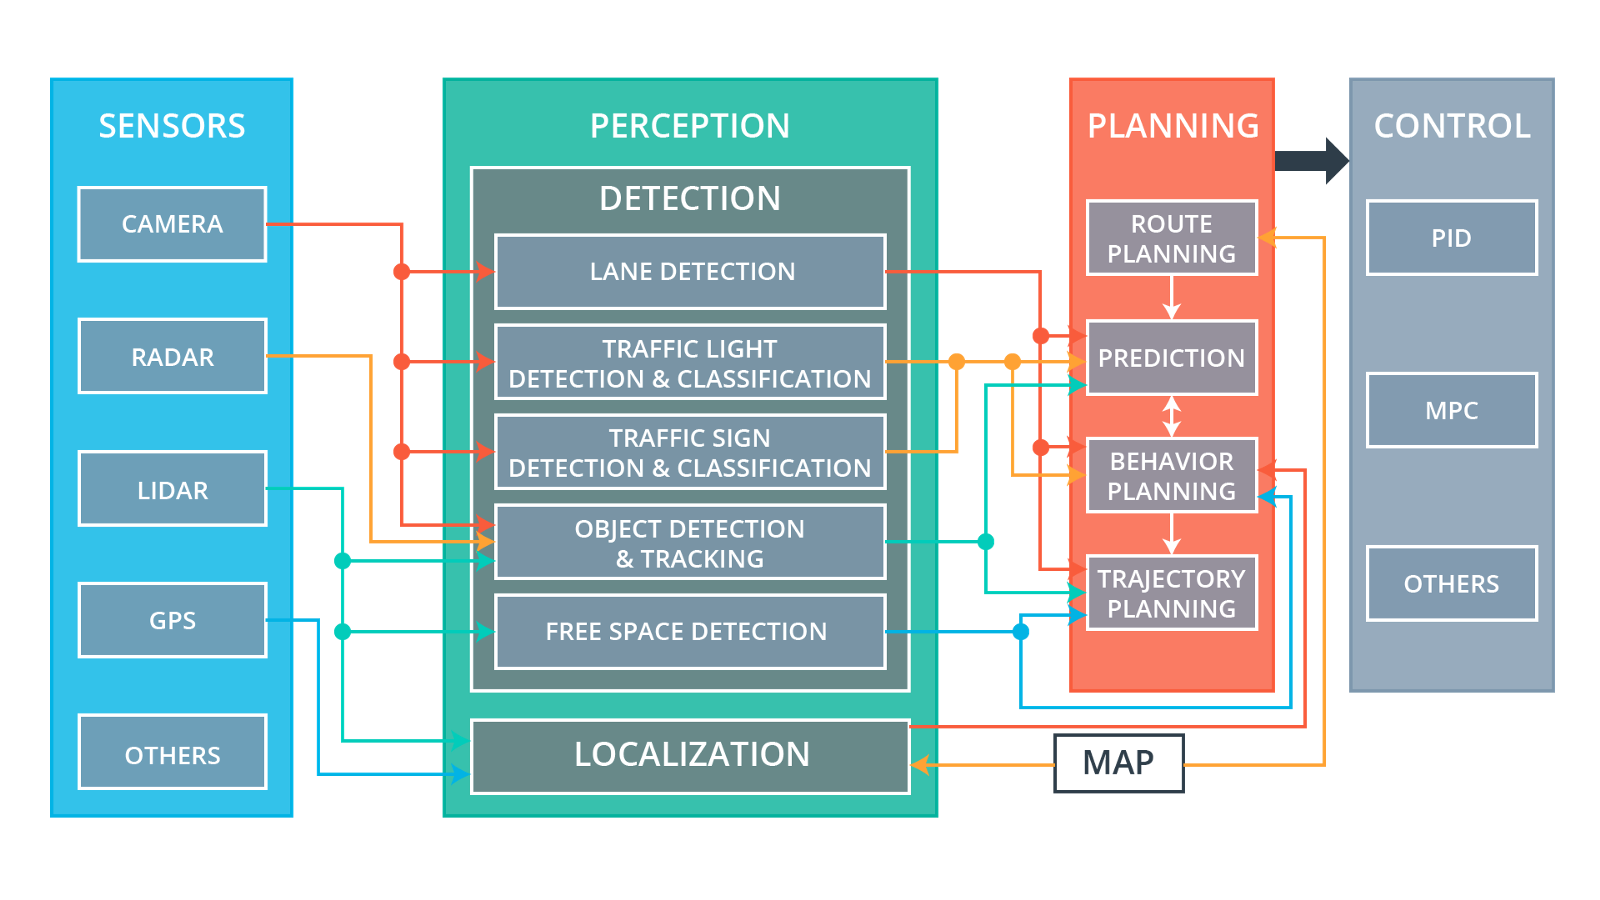
\includegraphics[width = 0.8 \textwidth ]{ADArchtiecture.png}
    \caption[Architektur autonomer Fahrzeuge]{Architektur eines autonomen fahrenden Fahrzeuges \gls{medium}}
    \label{fig:ADArchtiecture}
\end{figure}

F\"ur die maschinelle Wahrnehmung kann entweder ein kartenbasierter Ansatz oder ein rein sensorischer Ansatz genutzt werden.
Bei einem kartenbasierten Ansatz werden Eigenschaften des statischen Verkehrsraums in einer Karte hinterlegt \cite{Ziegler2017}. 
Solche Eigenschaften sind beispielsweise der Verlauf von Fahrstreifen. 
Es k\"onnen ebenfalls Informationen wie Geschwindigkeitsbegrenzungen oder Vorfahrtsregelungen hinterlegt werden. 
Hierdurch sind f\"ur das Fahrverhalten grundlegende Informationen direkt vorhanden und k\"onnen schnell abgerufen werden. 
F\"ur einen kartenbasierten Ansatz wird jedoch ein zus\"atzliches Lokalisationsmodul notwendig.
Aufgabe dieses Lokalisationsmodules ist es, die Position des Fahrzeuges relativ zur Karte zu bestimmen.
Hierzu k\"onnen unter anderem GPS basierte, eigenbewegungsbasierte oder kartenbasierte Positionssch\"atzungen  genutzt werden. 
H\"aufig ergibt sich die Positionssch\"atzung aus einer probabilistischen Kombination der vorher genannten Varianten. 
Diese Informationen m\"ussen bei rein sensorischer Wahrnehmung erst noch generiert werden, was eine hohe Anforderung an das Wahrnehmungsmodul darstellt. 
Die rein sensorische Wahrnehmung hat allerdings den Vorteil, dass keine Lokalisation mehr notwendig ist und dass sie unsensibel gegen\"uber Ver\"anderungen der als statisch angenommen Umgebung ist.
Ein detaillierte Karte mit Fahrstreifenverl\"aufen ist nicht notwendig.
Doch auch bei einem rein sensorischen Ansatz m\"ussen grundlegende Stra{\ss}eninformation hinterlegt sein um die Route des Fahrzeuges planen zu k\"onnen.
In beiden F\"allen muss zus\"atzlich noch eine Wahrnehmung der dynamischen Umgebung stattfinden.
Teil der dynamischen Umgebung sind beispielsweise andere Verkehrsteilnehmer wie Fahrzeuge und Fu{\ss}g\"anger oder aber ein Ampellicht. \cite{Ziegler2017}

Aus den in der Wahrnehmung generierten Daten wird ein Lagebild mit den Informationen zur Fahrzeugumgebung erzeugt \cite{Ziegler2017}. 
Dieses Lagebild wird im Planungsmodul, welches sich dem Wahrnehmungsmodul anschlie{\ss}t, genutzt. 
Neben der Trajektorienplanung k\"onnen auch die Routenplanung, die Pr\"adiktion und die Man\"overplanung zum Planungsmodul gez\"ahlt werden. 
In der Routenplanung wird in einem gegebenen Stra{\ss}ennetz die optimale Route zwischen zwei geographischen Positionen ermittelt \cite{Zhang2013}. 
Diese Aufgabe \"ahnelt der Aufgabe die bei menschlich gef\"uhrten Fahrzeugen heute h\"aufig von einem Navigationssystem \"ubernommen wird. 
In der Pr\"adiktion wird ausgehend vom aktuellen Zustand der Fahrzeuge pr\"adiziert wie sich eine Verkehrssituation in n\"achster Zukunft entwickeln wird.
Dabei werden die zuk\"unftigen Positionen und Zust\"ande der einzelnen Fahrzeuge vorherbestimmt \cite{Hermes2009}.


Die Man\"overplanung bestimmt ein Reihe von auszuf\"uhrenden Man\"overn.
Dies geschieht basierend auf der Fahraufgabe, welche sich aus der Routenplanung ableitet, dem angenommenen Verhalten anderer Verkehrsteilnehmer und der umgebenden Stra{\ss}e.
Ein Man\"over bestimmt das taktische Verhalten eines Fahrzeuges als Reaktion auf die lokale Fahrzeugumgebung. \cite{Zhang2013}
Ein typisches Man\"over ist ein Fahrstreifenwechsel. 
Aufgabe der Trajektorienplanung ist es nun anhand der gegebenen Informationen das Verhalten des eigenen Fahrzeuges in n\"achster Zukunft zu bestimmen \cite{Ziegler2017}. 

H\"aufig ist das Planungsmodul hierarchisch aufgebaut und die einzelnen Elemente besitzen nach unten hin abnehmende Planungshorizonte und Neuplanungsintervalle. 
So kann der Planungshorizont einer Routenplanung mehrere Stunden betragen und es kann eine vergleichsweise lange Zeit zwischen zwei Planungsschritten in Kauf genommen werden. 
Die Trajektorienplanung, als unterstes Glied der Hierarchie besitzt in der Regel einen Planungshorizont im Sekundenbereich und das Neuplanungsintervall kann im Millisekundenbereich liegen. 
Naumann und Stiller \cite{Naumann2017towards} zeigen jedoch, dass es nicht immer sinnvoll ist die einzelnen Planungsschritte getrennt voneinander durchzuf\"uhren.
In der von ihnen vorgestellten Arbeit zur kooperativen Verhaltensplanung wird die Pr\"adiktion und die Man\"overplanung in die Trajektorienplanung integriert.

Aufgabe des Regelungsmoduls, als letztes Glied der Kette ist es, das Fahrzeug entlang der aus dem Planungsmodul erhaltenen Solltrajektorie zu f\"uhren \cite{Ziegler2017}. 
Ein \"Uberblick der Gesamtarchitektur ist in Abbildung~\ref{fig:ADArchtiecture} gegeben.

Auch wenn die Begriffe Pfad und Trajektorie oft synonym verwendet werden soll an dieser Stelle auf deren Unterschied hingewiesen werden.  
So stellt ein Pfad die geometrische Verbindung zwischen einem Startzustand und einem Zielzustand dar. 
Eine zeitliche Komponente wird nicht ber\"ucksichtigt. 
Eine Trajektorie hingegen ber\"ucksichtigt die Zeit. 
Damit sind auch Information wie der Geschwindigkeitsverlauf in einer Trajektorie enthalten und es kann eine Kollisionspr\"ufung mit dynamischen Hindernissen durchgef\"uhrt werden. 
Diese Unterscheidung soll auch im Rahmen dieser Arbeit verwendet werden. \cite{Rathgeber2016}


\section{Optimierungsverfahren in der Trajektorienplanung}
Ziel der Optimierung ist die Ermittlung eines Optimums. 
Dieses Optimum soll in einem wohldefinierten Sinne optimal sein \cite{Ziegler2017}.
So kann mittels eines Navigationssystems die optimale Route im Sinne der geringsten Fahrzeit oder im Sinne des k\"urzesten Weges gesucht werden.
Ziel der Trajektorienplanung ist die Ermittlung einer optimalen Trajektorie \gls{symb:x_optTra} \( = (x(t), y(t))^T \). 
In diesem Kapitel soll zun\"achst eine Formulierung des Optimierungsproblems f\"ur die Trajektorieplanung stattfinden.
Anschlie{\ss}end sollen einige L\"osungsverfahren vorgestellt werden, die bei der Trajektorieplanung zum Einsatz kommen.


\subsection{Formulierung des Optimierungsproblems}
Generell k\"onnen Optimierungsprobleme zwei verschiedenen Gruppen zugeordnet werden. 
Statische Optimierungsprobleme und dynamische Optimierungsprobleme.

\begin{itemize}
\item \textit{Statisches Optimierungsproblem}: Minimierung einer Funktion mit Optimierungsvariablen,
die Elemente des Euklidischen Raumes sind.
\item \textit{Dynamisches Optimierungsproblem}: Minimierung eines Funktionals, bei dem die
Optimierungsvariablen Elemente des Hilbert"=Raumes sind (z.B. Zeitfunktionen). \cite{Graichen2012}
\end{itemize}

Wie in Kapitel \ref{Einordung_Trajktorieplanung} erl\"autert ist eine Trajektorie, im Gegensatz zum Pfad, eine zeitabh\"angige Funktion.
Damit wird deutlich, dass die dynamische Optimierung die f\"ur die Trajektorieplanung relevante Optimierung darstellt. 
Aus diesem Grund soll im Weiteren nur noch die dynamische Optimierung betrachtet werden.

Laut F\"ollinger \cite{Follinger1988} ist, um berechtigterweise von einer Optimierung zu sprechen, ein G\"utema{\ss} notwendig. 
Dieses G\"utema{\ss} ist eine Ma{\ss}zahl, durch welche die Qualit\"at eines Systemverhaltens bewertet wird.
Bei einem Trajektorieplanungsproblem wird damit also die Qualit\"at einer Trajektorie bewertet.
Ziel der Optimierung ist es nun, das G\"utema{\ss} entweder zu minimieren oder zu maximieren. 
Soll das G\"utema{\ss} minimiert werden, so wird das G\"utema{\ss} bei einer dynamischen Optimierung im Allgemeinen als Kostenfunktional bezeichnet.
Soll es maximiert werden, so kann von einem Belohnungsfunktional gesprochen werden.
Ob ein Kostenfunktional oder ein Belohnungsfunktional vorliegt spielt f\"ur die Optimierung kaum eine Rolle, da jedes Belohnungsfunktional in eine Kostenfunktional umgewandelt werden kann \cite{Graichen2012}.
Diese Eigenschaft ist durch das Dualit\"atsprinzip gegeben.
Daher kann im Weiteren von einem Kostenfunktional ausgegangenen werden, das es zu minimieren gilt.
Bei der Verwendung eines Kostenfunktionals ist jede Abweichung von der Optimaltrajektorie mit der Entstehung von Kosten verbunden.

Die zu ermittelnde Optimaltrajektorie soll nicht nur Kollisionsfreiheit garantieren sondern auch komfortabel sein.
Mit dem Ziel den Komfort und die Glattheit der Trajektorie zu steigern wird in der Literatur zur Trajektorienplanung h\"aufig die Geschwindigkeit, die Beschleunigung und der Ruck bei der Optimierung ber\"ucksichtigt \cite{Ziegler2017} \cite{Werling2011}.
Der Ruck ist die Ableitung der Beschleunigung nach der Zeit.
Das Kostenfunktional enth\"alt dann au{\ss}er der Trajektorienfunktion \gls{symb:x_optTra} \(=(x(t), y(t))^T \) auch ihre Ableitungen bis zum dritten Grad.
Damit ergibt sich eine Ruck"=Zeit"=optimale Trajektorie als L\"osung des Optimierungsproblems.
Das G\"utefunktional dieses Optimierungsproblems kann als

\begin{equation} 
  J = \int_{t_0}^{t_e} L( \pmb{x}, \pmb{\dot{x}}, \pmb{\ddot{x}}, \pmb{\dddot{x}}, t) dt
  \label{eq:Kostenfunktional}
\end{equation} 

formuliert werden (vgl. \cite{Ziegler2017}). Dabei stellen \( t_0\) und \( t_e\) den Anfangs- und Endzeitpunkt des Optimierungszeitraums dar.
Bei einer Trajektorienplanung wird dieser Optimierungszeitraums auch als Planungshorizont bezeichnet.

Zus\"atzlich zum Kostenfunktional m\"ussen Randbedingungen und in der Regel auch Nebenbedingungen festgelegt werden, die einzuhalten sind \cite{Follinger1988}.
Die Randbedingungen ergeben sich bei der Trajektorienplanung durch den Start- und  Endzustand des Fahrzeuges.
Vielmals soll in der Trajektorienplanung jedoch kein festdefinierter Endzustand festgelegt werden, da vielmehr ein Zielverhalten von Interesse ist. 
So ist beim Fahren auf einer Stra{\ss}e, \"ahnlich wie bei einem menschlichen Fahrer, weniger von Interesse an welcher Position sich das Fahrzeug am Ende des Planungshorizont befindet. 
Es ist eher von Interesse, dass sich das Fahrzeug noch immer in der Fahrbahnmitte befindet und mit einer Geschwindigkeit  f\"ahrt, die m\"oglichst nahe an der Wunschgeschwindigkeit ist.
Der Endpunkt des Optimierungsproblems ist somit nicht mehr vorgegeben sondern liegt innerhalb von einer Punktemenge des Zustandraumes, einer sogenannten Zielmannigfaltigkeit \(Z\) \cite{Follinger1988}. 

Die Nebenbedingungen ergeben sich aus \"au{\ss}eren und inneren Beschr\"ankungen. 
\"Au{\ss}ere Nebenbedingung betreffen die Umgebung des Fahrzeuges. 
Sie ergeben sich beispielsweise aus Hindernissen oder dem Stra{\ss}enverlauf. 
Dabei geht es immer um Kollisionsfreiheit. 
Die inneren Nebenbedingungen ergeben sich aus Grenzen der Fahrdynamik (zum Beispiel minimale Kurvenradien oder maximale Beschleunigungen) oder aus anderen Beschr\"ankungen wie zum Beispiel der Vorgabe einer maximalen Geschwindigkeit. \cite{Ziegler2017}
Diese Nebenbedingungen schr\"anken den Suchraum ein und k\"onnen entweder als Gleichungsbedingungen

\begin{equation} 
  f( \pmb{x}, \pmb{\dot{x}}, \pmb{\ddot{x}}, \pmb{\dddot{x}}, t) = 0
  \label{eq:Kostenfunktional}
\end{equation} 

oder als Ungleichungsbedingungen

\begin{equation} 
  h( \pmb{x}, \pmb{\dot{x}}, \pmb{\ddot{x}}, \pmb{\dddot{x}}, t) \leq 0
  \label{eq:Kostenfunktional}
\end{equation} 

ber\"ucksichtigt werden \cite{Papageorgiou1991}.
Ungleichungsbedingungen werden in vielen F\"allen ber\"ucksichtigt, indem sie in Gleichungsbedingungen transformiert werden.
Dies geschieht durch die Einf\"uhrung einer Schlupfunktion. \cite{Papageorgiou1991}

Sind das Kostenfunktional sowie Rand- und Nebenbedingungen gegeben, besteht das Optimierungsproblem nun darin, unter allen Trajektorien welche die Rand- und Nebenbedingungen erf\"ullen, diejenige zu finden, welche das Kostenfunktional zum globalen Minimum macht \cite{Follinger1988}.
Hierbei soll auf den Unterscheid zwischen einem globalen und einem lokalen Minimum hingewiesen werden.
Ein globales Minimum beschreibt das Minimum aller Vektoren, welche die Rand- und Nebenbedingungen erf\"ullen. 
Somit ergibt sich f\"ur ein Extremwertproblem, bis auf in sehr wenigen Ausnahmen, nur ein einziges globales Minimum. 
Ein lokales Minimum stellt hingegen nur ein Minimum in einer gewissen Umgebung dar. 
Nur falls es das einzige lokale Minimum ist, ist es auch sicher das globale Minimum. \cite{Follinger1988}


\begin{figure}[!htbp]
    \centering
    \subfigure[Mehrere lokale L\"osungen des Trajektorienplanungsproblems \cite{Ziegler2017}]{
        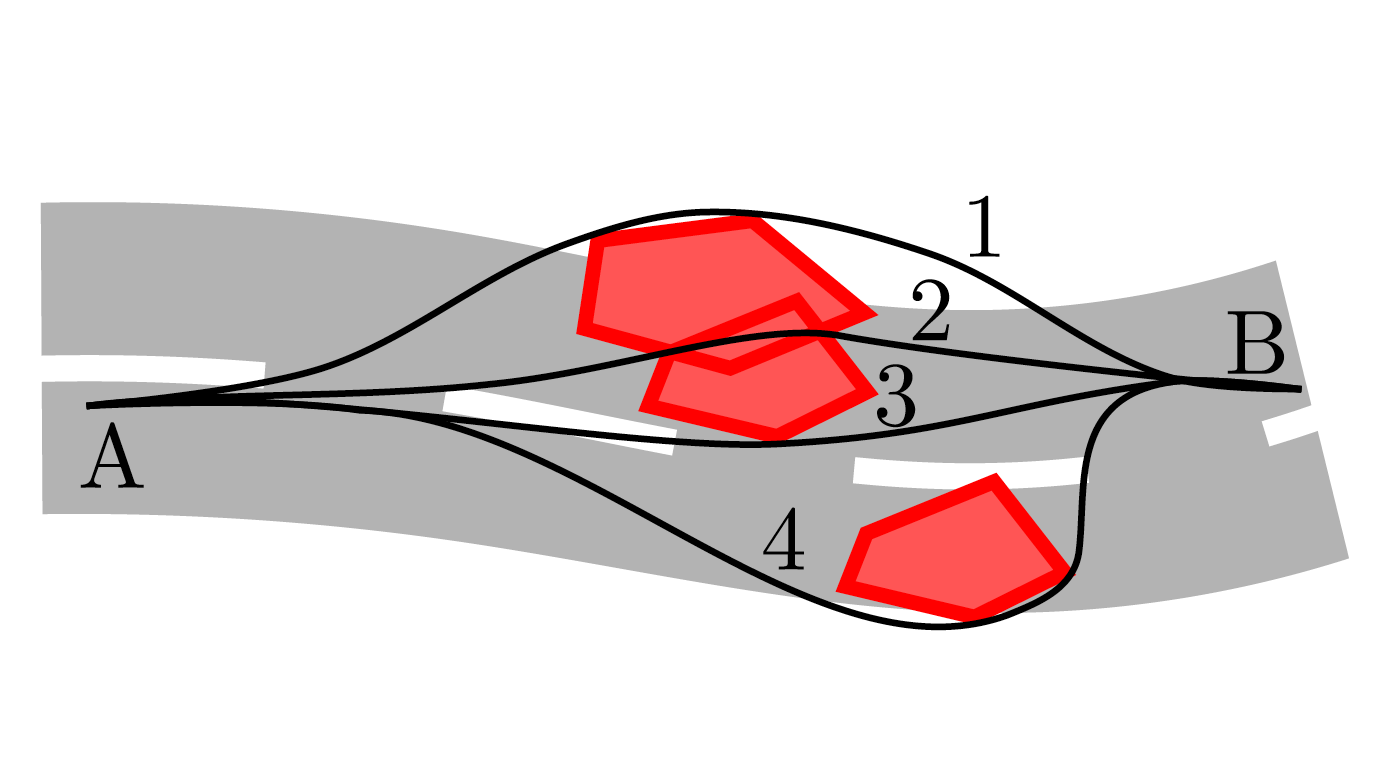
\includegraphics[width = 0.45 \textwidth]{LokalMinimum.png}
        \label{fig:LokalMinimum}
    }
    \hfill
     %add desired spacing between images, e. g. ~, \quad, \qquad, \hfill etc.
     %(or a blank line to force the subfigure onto a new line)
    \subfigure[Globale L\"osung des Trajektorienplanungsproblems \cite{Ziegler2017}]{
        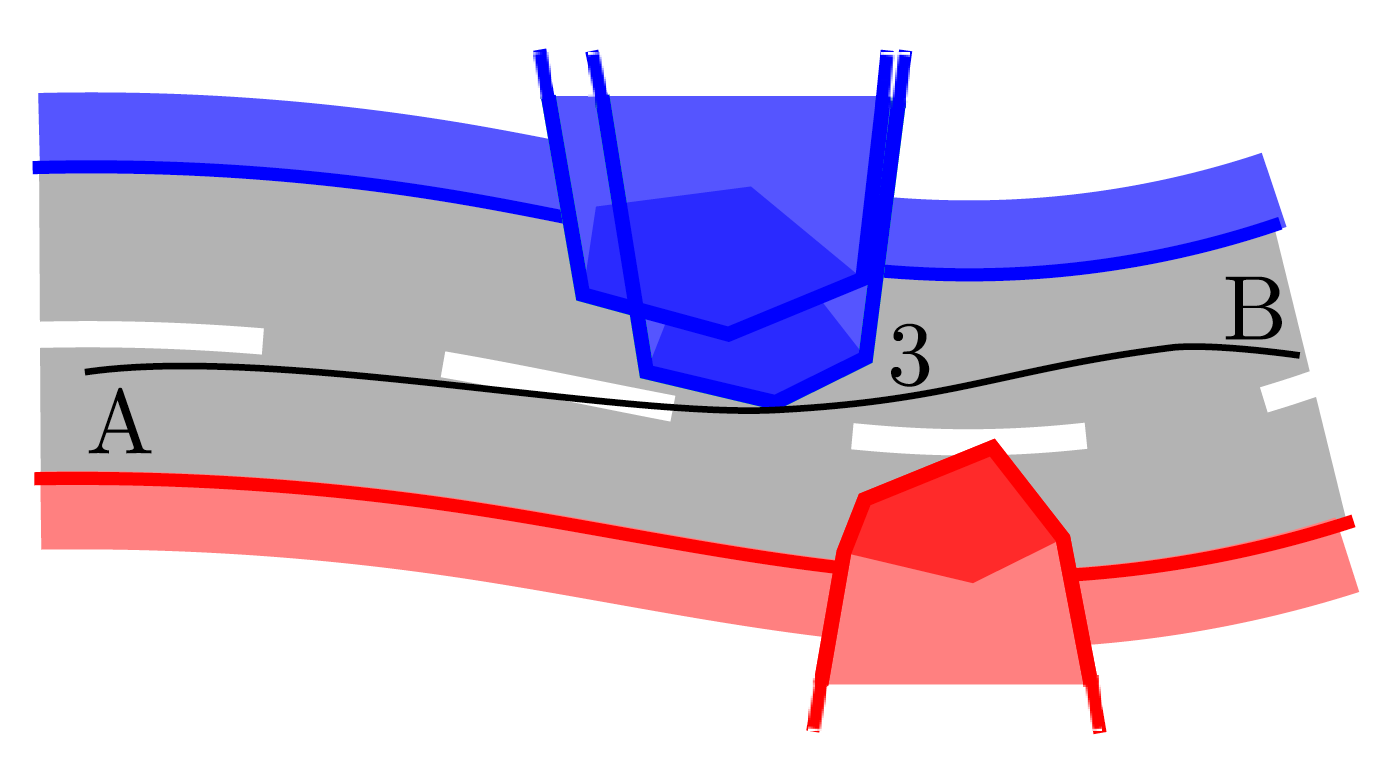
\includegraphics[width = 0.45  \textwidth]{GlobalesMinimum.png}
        \label{fig:GlobalesMinimum}
    }
    \caption[Anpassung f\"ur globales Minimum]{Anpassung des Trajektorienplanungsproblems zur Ermittlung des globalen Minimums}
    \label{fig:GlobalMinAdaption}
\end{figure}


Ziegler \cite{Ziegler2017} zeigt, dass es bedingt durch die Lage von Hindernissen zu mehreren lokalen Minima bei der Trajektorienplanung kommen kann. 
Dies ist in Abbildung~\ref{fig:LokalMinimum} dargestellt.
Nur eines von ihnen entspricht auch dem globalen Minimum.
Das ein gefundenes lokales Minimum das einzige im Suchraum ist und somit auch dem globalen Minimum entspricht kann nur bei konvexen Optimierungsproblemen sichergestellt werden.
Damit sich ein konvexes Optimierungsproblem ergibt, m\"ussen sowohl das Kostenfunktional als auch die Nebenbedingungen konvex sein. 
Ist ein Optimierungsproblem konvex, so k\"onnen im Allgemeinen einfachere und schnellere lokale L\"osungsverfahren genutzt werden. \cite{Graichen2012}
Somit stellt die Konvexit\"at eine wichtige Eigenschaft bei der Auswahl des L\"osungsverfahrens dar. 
Ist die Konvextit\"at nicht gegeben, kann versucht werden das Optimierungsproblem so anzupassen, dass sich ein konvexes Optimierungsproblem ergibt.
Eine Anpassung f\"ur das in Abbildung~\ref{fig:LokalMinimum} dargestellte Trajektorienplanungsproblem ist in Abbildung~\ref{fig:GlobalesMinimum} zu sehen.
Hier werden die Hindernisse jeweils einem Stra{\ss}enrand zugeordnet und die Polygone entsprechend nach au{\ss}en erweitert.
Dadurch f\"uhrt das Optimierungsproblem nur noch zu einem einzigen lokalen Minimum das dadurch auch gleichzeitig dem golbalen Minimum entspricht.

Im Folgenden sollen nun einige L\"osungsverfahren die in der Trajektorienplanung zum Einsatz kommen k\"onnen vorgestellt werden.



\subsection{Variationsrechnung}
\label{sec:Varationsrechnung}
Eine Vielzahl von L\"osungsverfahren beruhen auf der im Ende des 17. und Anfang des 18. Jahrhunderts entwickelten Variationsrechnung. 
Durch sie k\"onnen notwendige Bedingungen f\"ur das gesuchte Minimum abgeleitet werden und dadurch das Optimierungsproblem auf ein Randwertproblem zur\"uckgef\"uhrt werden.
Dies erm\"oglicht eine analytische L\"osung des Optimierungsproblems.
Analytische Verfahren k\"onnen in der Trajektorienplanung nur beschr\"ankt eingesetzt werden, da sie nur in sehr einfachen F\"allen angewendet werden k\"onnen. 
Eine analytische L\"osung ist nur dann m\"oglich, wenn keine expliziten Nebenbedingungen f\"ur Hindernisse, Stellbeschr\"ankungen und an die Fahrdynamik gestellt werden \cite{Ziegler2017}. \cite{Papageorgiou1991}

In vielen F\"allen kann das aus der Variationsrechnung abgeleitete Randwertproblem nur numerisch gel\"ost werden.
Ist dies der Fall wird von einem indirekten numerischen L\"osungsverfahren gesprochen.
Im Vergleich zu direkten numerischen L\"osungsverfahren, bei denen nicht das Randwertproblem sondern das Optimierungsproblem an sich numerisch gel\"ost wird, ist die Initialisierung schwieriger und die Ber\"ucksichtigung von Nebenbedingungen umst\"andlich \cite{Papageorgiou1991}. 
Allerdings ergeben Verfahren, die auf der Variationsrechnung beruhen hochgenaue L\"osungen und dadurch generiertes Wissen kann in der Trajektorienplanung genutzt werden.
So finden variationsrechnungsbasierte Ans\"atze in den Verfahren zur Trajektoriengenierung von Werling \cite{Werling2011} und Rathgeber \cite{Rathgeber2016} Anwendung. \cite{Papageorgiou1991}

F\"ur ein Minimum des Kostenfunktionals

\begin{equation} 
  J = \int_{t_0}^{t_e} L( x, \dot{x}, \ddot{x}, \dddot{x}, t) dt
  \label{eq:Kostenfunktional2}
\end{equation} 

mit der Funktion \(x(t)\), ergibt sich durch die Variationsrechnung folgende Differentialgleichung:

\begin{equation} 
  \frac{\delta L}{\delta x} - \frac{d}{dt} \left(\frac{\delta L}{\delta \dot{x}}\right) + \frac{d^2}{dt^2} \left(\frac{\delta L}{\delta \ddot{x}}\right) - \frac{d^3}{dt^3} \left(\frac{\delta L}{\delta \dddot{x}}\right) = 0
  \label{eq:EulerPoisson}
\end{equation} 

(vgl. \cite{Ziegler2017}). 
Sie wird als EULER"=POISSONschen Differenzialgleichung bezeichnet.
Unter Ber\"ucksichtigung der Anfangs- und Endbedingung ergibt die L\"osung dieses Randwertproblems, dass eine Ruck"=Zeit"=optimale Trajektorie durch ein Polynom 5. Ordnung dargestellt wird.
Diese wird sich in dem von Werling \cite{Werling2011} vorgestellten Verfahren zur Trajektorienplanung zu Nutze gemacht.
Hier wird jeweils f\"ur die laterale und die tangentiale Bewegung eine Schar von Polynomen 5. Ordnung generiert.
Dies geschieht zun\"achst getrennt von einander und ungeachtet von Nebenbedingungen. 
Zur Generierung der Polynomschar wird der Anfangszustand mit unterschiedlichen Endzust\"anden und Endzeitpunkten kombiniert. 
Im Anschluss werden die einzelnen L\"osungen der lateralen und tangentialen Bewegung miteinander kombiniert und auf Einhaltung der Nebenbedingungen untersucht. 
Die Kombination, welche die geringsten Kosten verursacht ergibt die angen\"aherte L\"osung des Optimierungsproblems.



\subsection{Direkte numerische Verfahren}
Bei direkten numerischen Verfahren wird das urspr\"ungliche dynamische Optimierungsproblem in ein statisches Optimierungsproblem umgewandelt. 
Dieses wird dann mittels numerischer Verfahren gel\"ost.
Gesucht wird nun nicht mehr die Funktion \gls{symb:x_optTra}(t) sondern die Positionen \(\pmb{x}_k, \pmb{x}_{k+1}, ..., \pmb{x}_N \) an diskreten St\"utzpunkten der Trajektorie.
Direkte numerische Verfahren wurden durch Fortschritt in der Speicherkapazit\"at und Prozessorleistung in den letzten Jahren immer popul\"arer. \cite{Papageorgiou1991}

Ein direktes numerisches Verfahren mit einer sehr hohen Genauigkeit ist das Kollokationsverfahren \cite{Papageorgiou1991}.
Es findet in dem von Ziegler \cite{Ziegler2017} vorgestellten lokalen, kontinuierlichen Verfahren zur Trajektorienplanung Anwendung. 
Bei Verfahren dieser Art wird durch eine zeitlich Diskretisierung des Problems der L\"osungsraum durch St\"utzstellen parametrisiert.
Die St\"utzstellen werden dann von der Optimaltrajektorie interpoliert.
F\"ur dieses Vorgehen wird das Integral des Kostenfunktionals durch eine endliche Summe ersetzt. 
Unter Verwendung des Finitdifferenzenverfahrens zur Berechnung der ersten und zweiten Ableitung wird das Kostenfunktional

\begin{equation} 
  J = \int_{t_0}^{t_e} L( x, \dot{x}, \ddot{x} , t) dt
\end{equation} 

durch

\begin{equation} 
  J = \sum_{i=1}^{n-2} L( t_i, x_i, \frac{\delta x_i}{2h}, \frac{\delta^2 x_i}{h^2} , h^2)h
\end{equation} 

ersetzt . Dabei gibt \(n\) die Anzahl der St\"utzpunkt an und \gls{symb:h} die Schrittweite.  \cite{Ziegler2017}
Es kann gezeigt werden, dass die L\"osung des statischen Ersatzproblems bei  \gls{symb:h} \(\to 0\) gegen die exakte L\"osung des Optimierungsproblems konvergiert \cite{Papageorgiou1991}.
In \cite{Ziegler2017} wird das statische Ersatzproblem durch das Verfahren der sequenziellen quadratische Programmierung (SQP) gel\"ost.
Dies ist ein Verfahren, um nichtlineare Optimierungsprobleme unter nichtlinearen Nebenbedingungen zu l\"osen


\subsection{Globale L\"osungsverfahren}
\label{globaleLV}
Beim Fahren in einer hochsturkturierten Umgebung, gegeben durch die Stra{\ss}e, entspricht die lokale L\"osung h\"aufig der globalen L\"osung \cite{Ziegler2017}.
Deshalb sind lokale L\"osungsverfahren in vielen F\"allen ausreichend.
Bei einer kooperativen Trajektorienplanung, die h\"aufig kombinatorische F\"ahigkeiten erfordert, ergeben sich jedoch in der Regel nichtkonvexe Optimierungsprobleme.
Somit muss hier in zumeist auf globale L\"osungsverfahren zur\"uckgegriffen werden, mit denen die L\"osung angen\"ahert wird.

\minisec{Randomisierte Verfahren}
Ein Ansatz zur Ermittlung von globalen L\"osungen bilden randomisierte Verfahren. 
Hierbei werden verschiedene L\"osungskandidaten zuf\"allig oder deterministisch generiert, anhand des Kostenfunktionals bewertet und anschlie{\ss}end der Kandidat mit den geringsten berechneten Kosten ausgew\"ahlt.
Allerdings sind solche L\"osungsverfahren nicht vollst\"andig da sie nicht terminieren, wenn f\"ur ein gegebenes Problem keine L\"osung existiert.
Weiter noch kann Optimalit\"at prinzipiell erst nach unendlich langer Laufzeit garantiert werden \cite{Ziegler2017}.
Da dies nicht m\"oglich ist muss aus rechenzeittechnischen Gr\"unden nach einer bestimmten Anzahl von L\"osungskandidaten oder nach einer bestimmten Zeit abgebrochen werden.
Die L\"osung ist nun der bis dahin beste L\"osungskandidat.
Sie entspricht einer Ann\"aherung an die optimale L\"osung.

Eine M\"oglichkeit die Qualit\"at der Versuch im Verlauf der Berechnung zu verbessern bieten metaheuristische Verfahren.
Damit ist es m\"oglich die exakte L\"osung schneller anzun\"ahern.
Basierend auf den bisher bekannten Informationen wird entschieden, welche L\"osungskandiaten als n\"achstes ausprobiert werden sollen.
Dieses Vorgehen wird als Ausbeutung (englisch: exploration) bezeichnet.
Es birgt jedoch die Gefahr gegen ein lokales Minimum zu konvergieren.
Deshalb muss auf ein gutes Verh\"altnis zwischen Ausbeutung und der Erkundung (englisch: exploitation) neuer Bereiche geachtet werden. \cite{Weise2009}

\minisec{Graphenbasierte Verfahren}
Graphenbasierte Verfahren bieten eine weitere M\"oglichkeit zur Ermittlung von global minimalen L\"osungen.
Sie werden h\"aufig zur Pfadgenerierung in unstrukturierter Umgebung angewandt \cite{Ziegler2017}.
Graphen bieten in der Optimierung eine Datenstruktur zur Modellierung von Optmierungsproblemen. 
Auf diese Datenstruktur kann dann ein Optimierungsverfahren angewandt werden.
Ein Graph ergibt sich aus einer Menge von Knoten und Kanten.
Die Knoten bilden diskrete Zust\"ande des L\"osungsraums ab.
Kanten stellen eine Verbindung zwischen zwei aufeinander folgende Konten dar.
Die Kanten k\"onnen gewichtet werden.
Die Gewichtung stellt die Kosten dar um von einem diskreten Zustand in den n\"achsten zu gelangen. 
Ein Graph mit gewichteten Kanten ist beispielhaft in Abbildung~\ref{fig:Graph} abgebildet.
Die Kantengewichte werden anhand einer Kostenfunktion ermittelt.
Ein Pfad ergibt sich nun aus der Abfolge von Knoten, die mit dem Startknoten beginnt und mit dem Zielknoten endet.
Die Kosten des Pfades ergeben sich aus der Summe der Gewichte aller Kanten die dabei abgefahren werden. \cite{Ziegler2017}
Ziel der Optimierung ist es nun den Pfad zu finden, f\"ur den die Summe der Kantengewichte minimal ist.

Die dynamische Programmierung bietet eine M\"oglichkeit diese L\"osung effizient zu finden.
Sie beruht auf dem Prinzip von Bellman.
Es besagt:

\begin{quote}
    \glqq Die Gesamtstrategie kann nur dann optimal sein, wenn jede Reststrategie optimal ist, ganz gleich, von welchem Zwischenstand. \grqq{}
\end{quote}

Basierend auf dieser Aussage kann das Optimierungsproblem auf einen mehrstufigen Entscheidungsprozess zur\"uckgef\"uhrt werden. 
Dazu wird zur Ermittlung der optimalen L\"osung im k-ten Schritt auf die optimale L\"osung im vorangegangenen Schritt zur\"uckgegriffen und diese als Endst\"uck der L\"osung des k-ten Schrittes verwendet. 
Diese Strategie ist durch die Rekursionsformel von Bellman beschrieben, die sich direkt aus dem Optimalit\"atsprinzip von Bellman ableitet. 
Beruhend auf dieser Formel wurden zahlreiche Suchverfahren entwickelt. 
Zwei der bekanntesten sind die h\"aufig verwendeten Suchalgorithmen Dijkstra und A*. \cite{Follinger1988}

\begin{figure}[!htbp]
    \centering
    \subfigure[Darstellung eines gewichteten Graphens \cite{Grimme2018}]{
        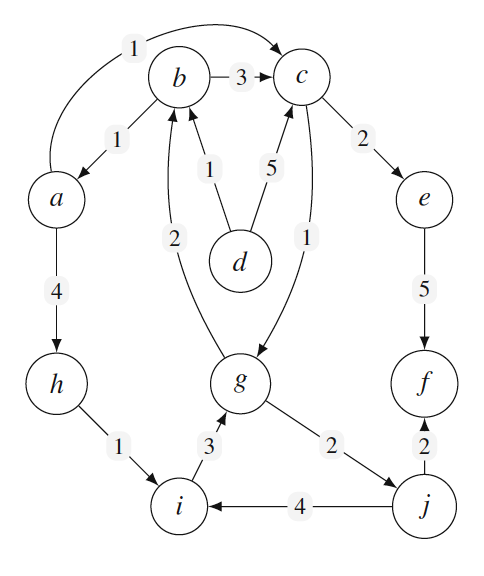
\includegraphics[width = 0.31 \textwidth]{Graph.png}
        \label{fig:Graph}
    }
    \hfill
     %add desired spacing between images, e. g. ~, \quad, \qquad, \hfill etc.
     %(or a blank line to force the subfigure onto a new line)
    \subfigure[Gitter aus Grundgeometrien \cite{Ziegler2009}]{
        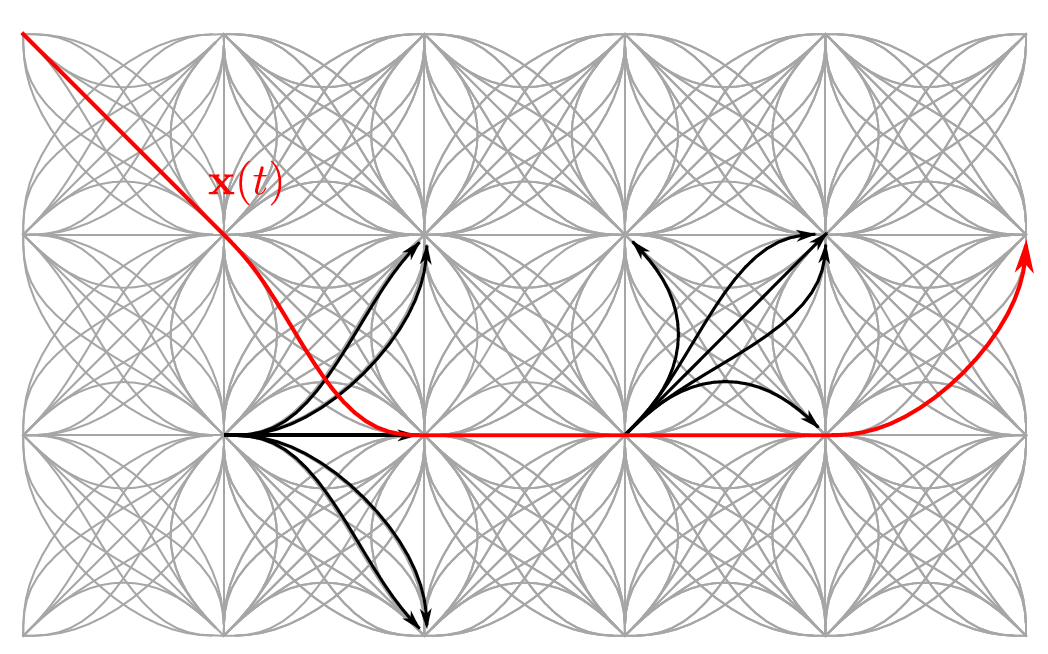
\includegraphics[width = 0.59  \textwidth]{statelatice.png}
        \label{fig:statetlatice}
    }
    \caption[Graphenbasierte Trajektorienplanung]{Graphenbasierte L\"osungsverfahren zur Trajektorienplanung}
    \label{fig:Graphenbasiert}
\end{figure}

Aufgabe der Trajektorienplanung ist es nun die Erstellung eines geeigneten Graphen sowie die Ermittlung der optimalen Trajektorie mittels eines geeigneten Suchalgorithmus.
Der Graph kann basierend auf einer sogenannte Zustandsraumvergitterung (englisch: state lattice) erstellt werden.
Dabei stellen die Gitterpunkte m\"ogliche Zust\"ande des Fahrzeuges dar.
Der Zustand kann zum Beispiel durch die Position und die Orientierung des Fahrzeuges, sowie die Kr\"ummung der Trajektorie beschrieben werden.
Die einzelnen Gitterpunkte werden dann durch einige wenige optimale Grundgeometrien verbunden. 
Die Grundgeometrien sind das Ergebnis eines lokalen Trajektorienplanungsproblems.
Sie ber\"ucksichtigen die inneren Nebenbedingungen und sorgen somit daf\"ur, dass die gefundene Trajektorie fahrbar ist.
Die optimale Trajektorie ergibt sich nun aus einer Kombination der Grundgeometrien.
Sie wird mit Verfahren der dynamischen Programmierung ermittelt. 
Ein solches Gitter aus Grundgeometrien sowie eine zusammengesetzte Beispieltrajektorie (in rot abgebildet) sind in Abbildung~\ref{fig:statetlatice} dargestellt.  \cite{Ziegler2009}



\section{Kooperative Verhaltensplanung}
Laut \cite{Naumann2017towards} und \cite{Lenz2016} ist es wichtig, dass automatisierte Fahrzeuge ein menschen\"ahnliches Fahrverhalten zeigen. 
Daf\"ur gibt es verschiedene Gr\"unde. 
Auf der einen Seite ist ein menschen\"ahnliches Verhalten wichtig, damit nicht automatisierten Fahrzeugen die Pr\"adiktion der automatisierten Fahrzeuge erm\"oglicht bzw. erleichtert wird. 
Auf der anderen Seite ist eine komfortables und menschen\"ahnliches Verhalten wichtig um die Akzeptanz von automatisierten Fahrzeugen zu steigern \cite{Naumann2017towards}. 

Eine essentielle Eigenschaft menschlicher Fahrer ist, dass die Absichten anderer Verkehrsteilnehmer prognostiziert werden und dass diese Absichten dann in der eigenen Verhaltensplanung Ber\"ucksichtigung finden. 
Ein solches Verhalten kann als kooperatives Verhalten gewertet werden. \cite{Lenz2016} 
Situationen in den menschliche Fahrer h\"aufig kooperatives Verhalten zeigen, kommen im realen Verkehr regelm\"a{\ss}ig vor. 
Ulbrich et al. \cite{Ulbrich2015} geben eine knappe \"Ubersicht solcher Situationen. 
Ein h\"aufig vorkommendes Beispiel, in denen menschliche Fahrer \"ublicherweise kooperatives Verhalten zeigen, ist das Auffahren auf die Autobahn. 
Hier kann oft beobachtet werden, dass Fahrzeuge ihre Geschwindigkeit anpassen um Fahrzeugen auf der Beschleunigungsspur das Auffahren zu erleichtern.

Ein solches kooperatives Verhalten ist in manchen Verkehrssituationen nicht nur erstrebenswert sondern sogar eine Voraussetzung f\"ur die erfolgreiche Meisterung der Situation \cite{Lenz2016}. 
Es wird offensichtlich, dass daher ein kooperatives Verhalten auch in der Trajektorienplanung von hochautomatisierten Fahrzeugen ber\"ucksichtigt werden sollte. 
Die meisten bisher bekannten Verfahren zur Trajektorienplanung zeigen jedoch lediglich ein reaktives Verhalten.
Dabei werden andere Verkehrsteilnehmer als bewegte Hindernisse betrachtet.
Der Einfluss des Verhaltens des Ego"=Fahrzeuges auf andere Verkehrsteilnehmer wird zumeist missachtet.
Sind kombinatorische F\"ahigkeiten gefragt, geraten solche Verfahren meist an ihre Grenzen.
Aus diesem Grund sind kooperative Ans\"atze zur Verhaltensplanung von hochautomatisierten Fahrzeugen vermehrt ins Forschungsinteresse ger\"uckt. \cite{Naumann2017towards}

Um ein kooperatives Verhalten in der Trajektorienplanung zu ber\"ucksichtigen ist es zun\"achst einmal wichtig zu betrachten, was ein kooperatives Verhalten ausmacht und wie dieses definiert werden kann. 
In der Literatur sind zahlreiche Definition f\"ur kooperatives Verhalten zu finden. 
So beschreiben Cao et al. \cite{Cao1997}, dass ein System mit mehreren Robotern ein kooperatives Verhalten aufweist, wenn \glqq ein zugrundeliegender Mechanismus f\"ur eine Erh\"ohung des Gesamtnutzen sorgt\grqq{}. 
Doran et al. \cite{Doran1997} beschreiben, dass Kooperieren bedeutet, dass \glqq mit anderen zusammen gehandelt wird um einen gemeinsamen Zweck oder einen gemeinsamen Vorteil zu erreichen\grqq{}. 
In psychologischer Betrachtung kann die Kooperation als eine Form der sozialen Zusammenarbeit zwischen Personen, Gruppen oder Institutionen gesehen werden \cite{Spiess2014}.

In den Ver\"offentlichungen von Naumann et al. \cite{Naumann2017} und Ulbrich et al. \cite{Ulbrich2015} findet jeweils eine Einteilung von kooperativem Verhalten statt. 
Naumann et al. stellen zur Einteilung des kooperativen Verhaltens ein Stufenmodell bestehend aus 5 Stufen vor, wobei von Stufe zu Stufe der Kooperationsgrad gesteigert wird. 
Die Klassifizierung findet anhand der Kenntnisse eines Agenten \"uber den Gesamtnutzen statt. 
Diese Einteilung ist in Tabelle~\ref{tab:koopStufenmodell} gegeben.

\begin{table}
  \centering
  \begin{tabular}{l p{5cm} p{8cm}}
  \hline
  Stufe& Klassifizierung 					& Kenntnis des Gesamtnutzens \\
  \hline
  0   	& unkooperatives Verhalten           		& keine Kenntnis des Gesamtnutzens \\
  1 	& reaktives Verhalten                      		& Kenntnis des Faktors Unfallfreiheit \\
  2 	& vorausschauendes Verhalten 		& Kenntnis einzelner Handlungsoptionen je Verkehrsteilnehmer \\
  3     	& bewusst kooperatives Verhalten 		& Kenntnis mehrerer Handlungsoptionen und deren wechselseitige Abh\"angigkeit je Verkehrsteilnehmer  \\
  4 	& ganzheitlich kooperatives Verhalten	& Kenntnis der m\"oglichen Handlungsoptionen aller relevanten Verkehrsteilnehmer und deren teilnehmer\"ubergreifende wechselseitige Abh\"angigkeit \\
  \hline
  \end{tabular}
  \caption[Kooperatives Stufenmodell]{Stufenmodell zur Einteilung von kooperativen Verhalten \cite{Naumann2017}}
  \label{tab:koopStufenmodell}
\end{table}

In \cite{Ulbrich2015} werden anhand einer Matrix mehreren m\"oglichen Kommunikationskan\"alen die f\"ur eine kooperatives Verhalten genutzt werden k\"onnen, verschiedene Level von kooperativen F\"ahigkeiten gegen\"uber gestellt. Die entsprechende Matrix ist in Abbildung~\ref{fig:coopMatrice} dargestellt.
Es wird ersichtlich, dass eine sogenannte Fahrzeug"=zu"=Fahrzeug"=Kommunikation, bei der explizite Kommunikationskan\"ale genutzt werden um Informationen und auch Intentionen zwischen zwei Fahrzeugen auszutauschen, nur einer der m\"oglichen Kommunikationskan\"ale ist. 
Eine solche Kommunikation war bereits h\"aufig Gegenstand von Untersuchungen, da sie ein hohes Potential an Komfort-, Effizienz-, und Sicherheitssteigerung verspricht. 
Allerdings werden sich automatisierte Fahrzeuge in absehbarer Zeit die Stra{\ss}e vor allem mit menschlich gef\"uhrten Fahrzeugen teilen, die nicht \"uber ein solches Kommunikationssystem verf\"ugen.
Andere Kommunikationsk\"anale wie zum Beispiel gewollte und ungewollte Gesten stellen hohe Anforderungen an die maschinelle Wahrnehmung, die heutige Wahrnehmungsysteme h\"aufig noch nicht erf\"ullen. 
Ein M\"oglichkeit ist jedoch, die Intension andere Fahrkehrsteilnehmer durch ihr Fahrverhalten zu pr\"adizieren und anhand dieser Informationen eine kooperative Trajektorienplanung zu realisieren. \cite{Ulbrich2015}

\begin{figure}[!htbp]
    \centering
    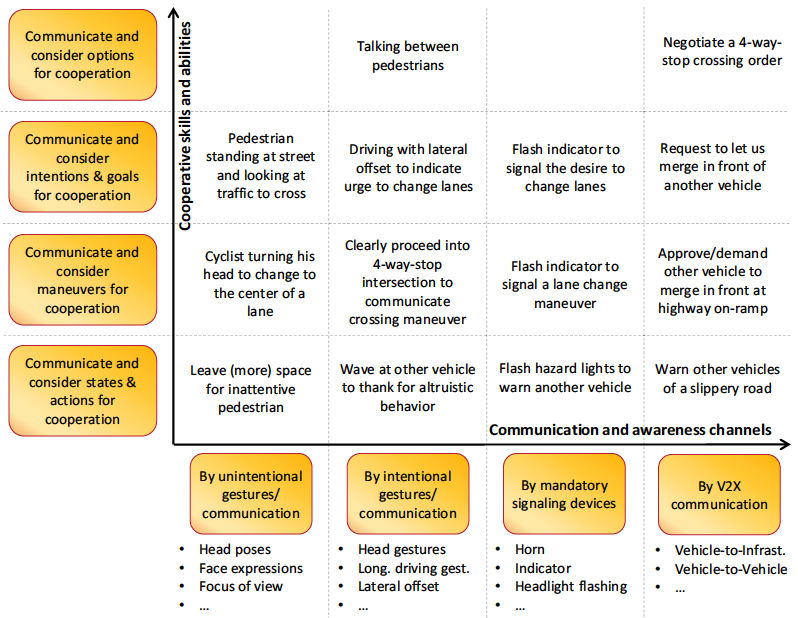
\includegraphics[width = \textwidth ]{KooperationsMatrix.png}
    \caption[Kooperationsmatrix]{Klassifizierung von kooperativer Verhaltensplanung anhand m\"oglicher Kommunikationskan\"ale und notwendigen F\"ahigkeiten \cite{Ulbrich2015}}
    \label{fig:coopMatrice}
\end{figure}




\FloatBarrier


\section{Frenet Koordinatensystem}
\label{sec:Frenet}
Zur Beschreibung der Fahrzeugbewegung stehen verschiedene Koordinatensysteme zur Verf\"ugung. 
G\"angige Koordinatensysteme die in der Bewegungsplanung genutzt werden sind das weltfeste Koordinatensystem, das fahrzeugfeste Koordinatensystem und das Stra{\ss}enkoordinatensystem. 
Abbildung~\ref{fig:FrenetKoord} gibt eine \"Ubersicht \"uber die verschiedenen Koordinatensysteme.
Die Wahl des Koordinatensystems kann starke Auswirkungen auf die Komplexit\"at und somit auch auf die Laufzeit eines Planungsalgorithmus haben. 
Somit spielt die Wahl eines geeigneten Koordinatensystems eine wichtige Rolle in der Trajektorienplanung.
Im Folgenden soll nun das Frenet"=Koordinatensystem vorgestellt werden und seine Nutzung f\"ur die Trajektorienplanung dieser Arbeit motiviert werden.
Eine Beschreibung in Frenet"=Koordinaten entspricht der mathematischen Beschreibung des Stra{\ss}enkoordinatensystems. \cite{Rathgeber2016}

Eine entscheidende Eigenschaft die sich durch die Wahl des Frenet"=Koordinatensystems ergibt ist, dass nicht in Weltkoordinaten geplant wird, sondern entlang einer Referenzkurve.
H\"aufig ist nicht die globale Position des Fahrzeuges relevant, sondern die Position des Fahrzeuges relativ zur Fahrspur und zu anderen Verkehrsteilnehmern \cite{Rathgeber2016}.
Beim Fahren auf einer Stra{\ss}e kann entweder die Fahrbahnmitte oder der linke oder rechte Fahrbahnrand als Referenzkurve gew\"ahlt werden. 
Im Falle einer unstrukturierten Umgebung, beispielsweise beim Fahren auf einer Parkfl\"ache, ist die Referenzkurve das Ergebnis einer Pfadsuche.  \cite{Werling2011}

\begin{figure}[!htbp]
    \centering
    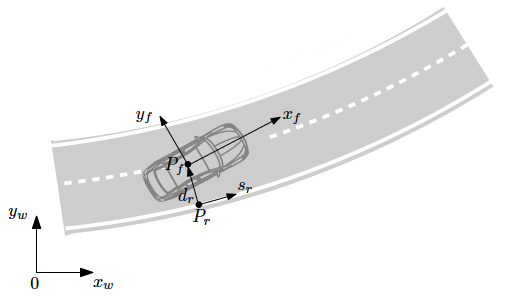
\includegraphics[width = 0.8 \textwidth]{FrenetKoordinaten.png}
    \caption[Koordinatensysteme]{\"Ubersicht \"uber die verwendeten Koordinatensysteme. Dargestellt ist das weltfeste Koordinatensystem (\(F_w = \{0, x_w, y_w\}\)), das fahrzeugfeste Koordinatensystem (\(F_f = \{P_f, x_f, y_f\}\)) und das Stra{\ss}enkoordinatensystem beschrieben in Frenet"=Koordinaten (\(F_r = \{P_r, s_r, d_r\}\)). \cite{Rathgeber2016}}
    \label{fig:FrenetKoord}
\end{figure}

Die Fahrzeugposition wird nun durch die Bogenl\"ange \gls{symb:s_r} entlang der Referenzkurve und den Abstand \gls{symb:d_r} zur Referenzkurve beschrieben. 
Dabei zeigt \gls{symb:s_r} in Richtung des Tangentenvektors \(t({s_r})\) und \gls{symb:d_r} zeigt in Richtung des Normalenvektors \(n({s_r})\).
Der Tangenetenvektor \(t({s_r})\) ist immer tangential zur Referenzkurve ausgerichtet. 
Der Normalenvektor \(n({s_r})\) steht senkrecht zu \(t({s_r})\) und zeigt auf den Referenzpunkt \({P_f}\) des Fahrzeuges. \cite{Rathgeber2016}

Im Planungsmodul wird nun nicht die Bewegung in Richtung \(x_f\) geplant, welche die Richtung entlang der geplanten Trajektorie darstellt.
Stattdessen wird die Bewegung des Fu{\ss}punktes \(P_r\) entlang der Referenzkurve geplant. 
Dadurch ist es m\"oglich die sich ergebende Trajektorie geschlossen zu berechnen. \cite{Werling2011}

Nicht nur die Fahrzeugeigenbewegung, sondern auch alle anderen relevanten Verkehrsteilnehmer werden in Frenet"=Koordinaten betrachtet.
Die Transformation vom Welt- ins Frenet"=Koordinatensystem entspricht anschaulich einer Entkr\"ummung der Fahrbahn \cite{Rathgeber2016}. 
Dies ist in Abbildung~\ref{fig:Fahrbahnentkruemmung} dargestellt. 
Durch die entkr\"ummte Betrachtung der Verkehrssituation ergeben sich einige Vorteile. 
Es vereinfacht sich die Planung f\"ur die Vorgabe von Haltepunkten, sowie von Soll- und Sicherheitsabst\"anden \cite{Werling2011}. 
Au{\ss}erdem kann eine getrennte Optimierung der L\"angs- und Querbewegung des Fahrzeuges \cite{Rathgeber2016} stattfinden. 
Werling \cite{Werling2011} beschreibt des Weiteren, dass sich Vorteile bei der Planung eines Fahrstreifenwechsels auf einer gekr\"ummten Fahrbahn ergeben.
Demzufolge ergibt sich durch die Wahl des Frenet"=Koordinatensystem ein Fahrstreifenwechsel, der mehr einem menschlichen Fahrverhalten \"ahnelt.
Dadurch kann die Bewegung des Fahrzeuges von anderen Verkehrsteilnehmern leichter eingesch\"atzt werden.

\begin{figure}[!htbp]
    \centering
    \subfigure[Verkehrsituation auf gekr\"ummter Fahrbahn \cite{Rathgeber2016}]{
        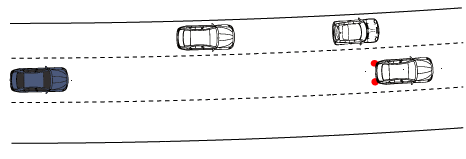
\includegraphics[width = 0.45 \textwidth ]{GekreummtFahrsituation.png}
        \label{fig:lGekruemmteFahrbahn}
    }
    \hfill
     %add desired spacing between images, e. g. ~, \quad, \qquad, \hfill etc.
     %(or a blank line to force the subfigure onto a new line)
    \subfigure[Entkr\"ummte Verkehrssituation \cite{Rathgeber2016}]{
        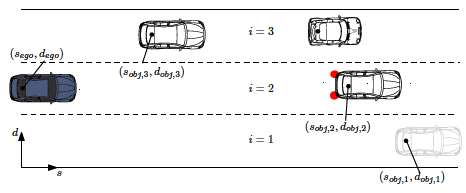
\includegraphics[width = 0.45 \textwidth ]{EntkreummtFahrsituation.png}
        \label{fig:EntkruemmteFahrbahn}
    }
    \caption[Fahrbahnentkr\"ummung]{Visualisierung der Entkr\"ummung der Verkehrssituation durch die Verwendung von Frenet"=Koordinaten}
    \label{fig:Fahrbahnentkruemmung}
\end{figure}

Die Formeln zur Umwandlung von Welt- in Frenet"=Koordinaten und umgekehrt sowie zur Berechnung der Bewegung entlang der Referenzkurve sind in \cite{Werling2011} und \cite{Rathgeber2016} gegeben.




\section{Verwandte Arbeiten}
F\"ur die kooperative Bewegungsplanung automatisierter Fahrzeuge existieren in der Forschung bereits einige Ans\"atze.
In vielen F\"allen wird ein kooperatives Verhalten erreicht indem im Kostenfunktional der Fahrzeuge auch die Kosten andere Verkehrsteilnehmer ber\"ucksichtigt werden.
An dieser Stelle werden nun zwei dieser Ans\"atze exemplarisch vorgestellt.


\subsection{Rekursive Konfliktl\"osung}
In \cite{Schwarting2014} wird ein Planungsalgorithmus f\"ur eine kooperative Verhaltensplanung in einer autobahn\"ahnlichen Umgebung vorgestellt. 
Dieser beruht auf  einer rekursiven Konfliktl\"osung.
F\"ur jedes in Betracht gezogenen Fahrzeug einzeln, beginnend mit dem am weitesten vorne fahrenden Fahrzeug, wird zun\"achst eine egoistische Planung durchgef\"uhrt. 
Basierend auf dieser egoistischen Planung werden dann Konflikte, die durch Interaktion mit anderen Fahrzeugen auftreten detektiert und anschlie{\ss}end \"uber einen Konfliktl\"osungsalgorithmus gel\"ost. 
Die Man\"over, die den Fahrzeugen zur Verf\"ugung stehen, werden durch sogenannte Bewegungsprimitive beschr\"ankt. 
Ein Bewegungsprimitiv wird dabei vollst\"andig beschrieben durch
\begin{itemize}
\item eine Beschleunigungskurve (beschleunige, halte Geschwindigkeit, bremse),
\item einen Bewegungstyp (Fahrstreifenwechsel auf die linke oder rechte Fahrstreifen Fahrstreifen beibehalten),
\item die Bewegungsdauer und
\item den Zeitpunkt der Initiierung.
\end{itemize}
Anstatt einer unendlichen Menge von M\"oglichkeiten stehen den Fahrzeugen somit nur wenige aber zweckm\"a{\ss}ige Man\"over zur Verf\"ugung. 
In Abbildung~\ref{fig:Motionprimit} ist ein Man\"oversatz f\"ur ein Fahrzeug in einer autobahn\"ahnlichen Situation dargestellt.

\begin{figure}[!htbp]
    \centering
    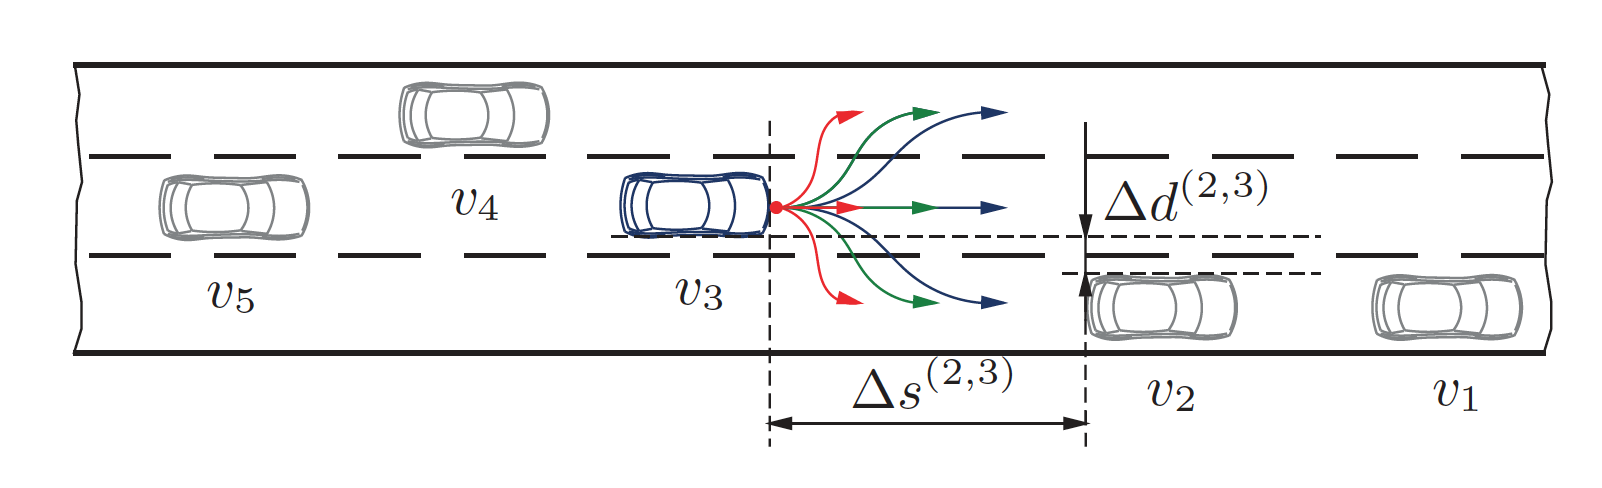
\includegraphics[width = 0.8 \textwidth ]{Motionprimit.png}
    \caption[Bewegungsprimitive]{Satz von m\"oglichen Man\"overn}
    \label{fig:Motionprimit}
\end{figure}

In der egoistischen Planung findet zun\"achst eine Planung statt in der die Interessen anderer Fahrzeuge missachtet werden. 
Endet der Fahrstreifen eines Fahrzeuges wird ein Zeitpunkt \(TTA_{LaneEnd}\) bestimmt, bei dem ein Fahrstreifenwechsel eingeleitet wird. 
Befindet sich vor dem zu betrachtenden Fahrzeug ein langsameres Fahrzeug auf der gleichen Fahrstreifen, wird ein Zeitpunkt \(TTA_{smart}\) bestimmt. 
Dieser Zeitpunkt gibt an, wann ein Fahrstreifenwechsel zum \"Uberholen eingeleitet werden soll. 
Zur Bestimmung von \(TTA_{smart}\) wird sowohl der Abstand, die Differenzbeschleunigung  und die Differenzgeschwindigkeit der Fahrzeuge in Betracht gezogen als auch die Wunschgeschwindigkeit des betrachteten Fahrzeuges.

Nachdem f\"ur alle Fahrzeuge die egoistische Bewegungsplanung durchgef\"uhrt wurde, kommt der rekursive Konfliktl\"osungsalgorithmus zum Einsatz. 
Daf\"ur wird, beginnend mit dem vordersten Fahrzeug, eine Konflikterkennung ausgef\"uhrt in der gepr\"uft wird, ob es durch die egoistische Planung zur Unterschreitung von Sicherheitsabst\"anden kommt. 
Dabei werden nur vorausfahrende Fahrzeuge in Betracht gezogen. 
Falls ein Konflikt detektiert wird, wird eine Konfliktl\"osung ermittelt. 
Daf\"ur werden alle m\"oglichen Man\"overkombinationen der beteiligten Fahrzeuge anhand einer Kostenfunktion bewertet. 
Anschlie{\ss}end wird die Man\"overkombination ausgew\"ahlt, welche die geringsten gemeinsamen Kosten der beiden Fahrzeuge verursacht. 
Dadurch wird ein kooperatives Verhalten aller Fahrzeuge abgebildet.

Wenn alle Fahrzeuge den Konfliktl\"osungsalgorithmus durchlaufen haben ist der Planungsschritt abgeschlossen. 
Die Gesamtl\"osung enth\"alt auch die L\"osung des Ego"=Fahrzeuges. 
Da das Ergebnis stark diskretisiert ist, wird vorgeschlagen dieses an einen Trajektorienplaner weiterzugeben.
Basierend auf dem diskertisierten Ergbnis soll dieser eine komfortable Trajektorie ermitteln.
Hierf\"ur kann der von Werling \cite{Werling2010} vorgestellte ruckminimierende Trajektoriengenerator genutzt werden.

Der Algorithmus wurde sowohl in einer Simulation als auch auf der Autobahn getestet. 
Den Autoren zufolge war der Algorithmus in der Lage Konflikte mit anderen Fahrzeugen zu antizipieren und zu l\"osen.
Es konnten dadurch sinnvolle Fahrman\"over erzeuget werden.

\subsection{Kooperative Planung mit Monte Carlo Tree Search}
Lenz et al. \cite{Lenz2016} stellen einen kombinatorischen Bewegungsalgorithmus basierend auf dem \gls{mcts} vor. 
Ein Baum ist in der Graphentheorie ein spezieller Typ von Graph \cite{Grimme2018}. 
Deshalb kann der vorgestellte Bewegungsalgorithmus zu den Graphen basierten Verfahren gez\"ahlt werden. 
Beim \gls{mcts} handelt es sich um eine randomisierte Suchmethode, welche die Pr\"azision einer Baumsuche mit der Allgemeing\"ultigkeit eines Samplingverfahrenes kombiniert \cite{Browne2012}. 
Der Basisalgorithmus kann in die vier Schritte: Selektion, Expansion, Simulation und R\"uckpropagierung eingeteilt werden. 
Die vier Schritte des Basisalgorithmus sind in Abbildung~\ref{fig:MCTS} visualisiert.

Dieser Basisalgorithmus wird abge\"andert, um ihn auf das Problem der kombinatorischen Bewegungsplanung anzupassen.  
Dazu wird die Planung zeitlich diskretisiert. 
Die in der Planung ber\"ucksichtigten Fahrzeuge k\"onnen Aktionen nur an den diskreten Zeitpunkten ausf\"uhren und tun dies alle simultan. 
Die Planung findet damit in Etappen statt. 
Au{\ss}erdem werden die in Betracht gezogenen Fahrzeuge in interagierende und beeinflusste Fahrzeuge unterteilt.
Die Unterteilung der Fahrzeuge hat Auswirkungen darauf, wie die Fahrzeuge im Planungsalgorithmus behandelt werden.
In Abbildungn~\ref{fig:Klassifizierung} ist die Einteilung der Fahrzeuge f\"ur ein autobahn\"ahnliches Scenario dargestellt.
Im Folgenden sollen nun kurz die einzelnen Schritte des angepassten Algorithmus erl\"autert werden.

\begin{figure}[!htbp]
    \centering
    \subfigure[Die vier Schritte des \gls{mcts} \cite{Browne2012}]{
        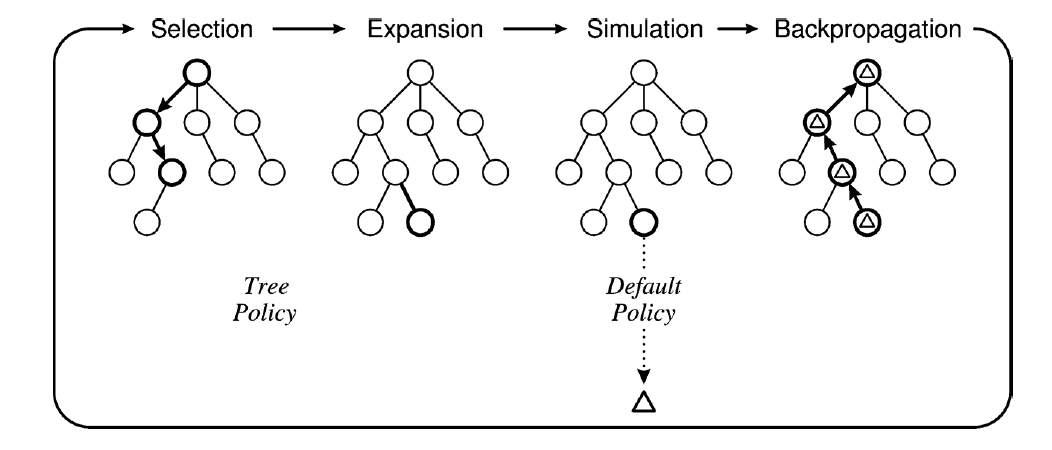
\includegraphics[width = 0.4 \textwidth ]{MCTS.png}
        \label{fig:MCTS}
    }
    \hfill
     %add desired spacing between images, e. g. ~, \quad, \qquad, \hfill etc.
     %(or a blank line to force the subfigure onto a new line)
    \subfigure[Klassifizierung der Fahrzeug (rot: Ego"=Fahrzeug, blau: interagierende Fahrzeuge, wei{\ss}: beeinflusste Fahrzeuge) \cite{Lenz2016}]{
        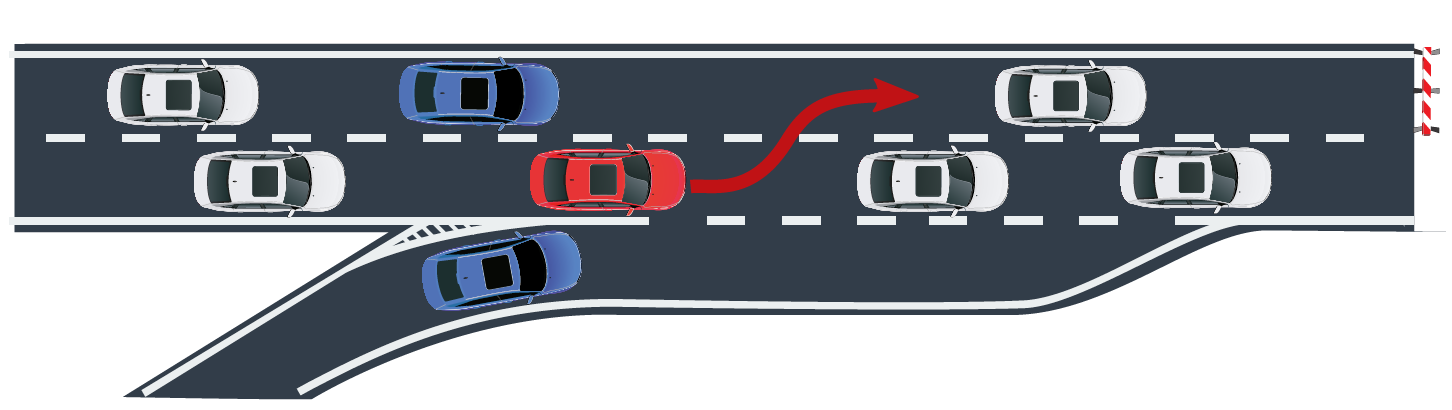
\includegraphics[width = 0.5 \textwidth]{Klassifizierung.png}
        \label{fig:Klassifizierung}
    }
    \caption[Monte Carlo Tree Search]{Kooperative Planung mit dem Monte Carlo Tree Search}
    \label{fig:koopMCTS}
\end{figure}


Im ersten Schritt, dem Selektionsschritt, wird ermittelt welcher Knoten als n\"achstes expandiert werden soll. 
Entsprechend eines gew\"ahlten Auswahlverfahrens wird der Baum nach unten durchlaufen, bis ein Endknoten (Blattknoten) erreicht wurde. 
Hier wurde auf einen gebr\"auchlichen Auswahlalgorithmus zur\"uckgegriffen.

Im Expansionsschritt werden dem nun Baum neue Knoten hinzugef\"ugt. 
Um die simultane Entscheidung der Fahrzeuge in einem Baum darstellen zu k\"onnen werden die Entscheidungen der Fahrzeuge zwar aufeinanderfolgend getroffen, aber bis zum R\"uckpropagierungsschritt verborgen. 
Interagierenden Fahrzeugen steht f\"ur die Entscheidung eine fest vordefinierte Menge von m\"oglichen Aktionen zur Verf\"ugung.
Beeinflusste Fahrzeuge verhalten sich entsprechend dem von Treiber et al. \cite{Treiber2000} vorgestellten \gls{idm}. 
Auf diese wird in Kapitel~\ref{sec:IDMpred} genauer eingegangen. 

Im Simulationsschritt wird nun ausgehend von den neuen Knoten eine Simulation durchgef\"uhrt, die den Ausgang pr\"adizieren soll. 
Als Standartverhalten der Fahrzeuge wird hier erneut das \gls{idm} verwendet. 
Die Kosten der neuen Knoten werden anhand der Kostenfunktion des jeweiligen Fahrzeuges bewertet.
In dieser werden neben Kosten die durch das Verhalten des eigenen Fahrzeuges bedingt sind \"uber einen Kooperationsfaktor auch die Kosten der anderen Fahrzeuge ber\"ucksichtigt. 
Somit wird davon ausgegangen, dass sich alle Fahrzeuge kooperativ verhalten.
Im letzten Schritt, dem R\"uckpropagierungsschritt, werden anhand des Simulationsergebnisses die Statistiken der Knoten entlang des gew\"ahlten Pfades aktualisiert.

Die vier beschriebenen Schritte werden solange wiederholt, bis der Algorithmus abgebrochen wird.
Dadurch werden immer mehr Knoten zum Baum hinzzugef\"ugt und somit immer mehr kombinatorische Bewegungsm\"oglichkeiten untersucht.

Die Autoren heben hervor, dass sich durch die Verwendung des \gls{mcts} mehrere Vorteile ergeben.
Dazu geh\"oren, dass der Algorithmus stark parallelisierbar ist und dass er jederzeit abgebrochen werden kann und ein valides Ergebnis zur\"uckgeben wird.
Der Algorithmus wurde simulativ in Fahrstreifenwechselszenarien verschiedener Komplexit\"at getestet. 
Es konnte gezeigt werden, dass der Algorithmus in der Lage ist ein menschen\"ahnliches kooperatives Fahrverhalten abzubilden.
Es wird au{\ss}erdem beschrieben, dass sich der Algorithmus selbst dann als robust herausgestellt hat, wenn die Kostenfunktion anderer Fahrzeuge falsch eingesch\"atzt wurde oder diese sich suboptimal verhalten.


     
% !TeX root = ../thesis.tex

\chapter{Basisalgorithmus und Annahmen}
\label{sec:underlying-conditions_preliminaries}
Naumann und Stiller stellen in \cite{Naumann2017towards} einen Algorithmus zur kooperativen Verhaltensplanung automatisierter Fahrzeuge vor.
Dieser Algorithmus dient als Ausgangspunkt der vorliegenden Arbeit und soll im Weiteren als Basisalgorithmus bezeichnet werden.
In diesem Kapitel soll zun\"achst dieser Basisalgorithmus mit seinen wichtigsten Bestandteilen beschrieben werden.
Anschlie{\ss}end sollen Annahmen, die dem in dieser Arbeit vorgestellten Trajektorienplanungsalgorithmus zugrundeliegen, angegeben werden.


\section{Basisalgorithmus}
Naumann und Stiller \cite{Naumann2017towards} stellen einen Bewegungsplanungsalgorithmus vor, bei dem die Pr\"adiktion anderer Verkehrsteilnehmer in die Bewegungsplanung integriert wird.
Dies geschieht, indem im Optimierungsproblem nicht die Trajektorie Ego"=Fahrzeuges ermittelt wird, sondern die der anderen relevanten Fahrzeuge auch.
Das Ergebnis des Planungsalgorithmus ist demnach nicht mehr nur die optimale Trajektorie des Ego"=Fahrzeuges \gls{symb:x_optTra} \( = (x(t), y(t))^T \), sondern ein Trajektorienenset \gls{symb:x_Traset} \(= (\pmb{x}_1, \pmb{x}_2, ...) \), das aus den Trajektorien der einzelnen Fahrzeuge besteht.
Aus dem Optimierungsproblem wird somit ein Multi"=Agenten"=Optimierungsproblem.
Durch diese Multi"=Agenten"=Optimierung wird nicht nur ber\"ucksichtigt, dass andere Fahrzeuge das Verhalten des Ego"=Fahrzeuges beeinflussen sondern auch, dass das Ego"=Fahrzeug das Verhalten der anderen Verkehrsteilnehmer beeinflusst.
Die Verhaltensplanung des Ego"=Fahrzeuges ist damit nicht mehr rein reaktiv sondern kann nach \cite{Naumann2017} als kooperativ gewertet werden.

F\"ur dieses Mulit"=Agenten"=Optimierungsproblem wird ein neues Kostenfunktional vorgestellt, das au{\ss}er den Kosten des Ego"=Fahrzeuges auch die Kosten der anderen relevanten Fahrzeug enth\"alt.
Durch die Multi"=Agenten"=Optimierung ergibt sich ein stark nicht konvexes Optimierungsproblem, das nicht durch lokale Verfahren gel\"ost werden kann. 
Deshalb wird au{\ss}erdem ein globales, samplingbasiertes L\"osungsverfahren vorgestellt.
In den folgenden Abschnitten soll nun zun\"achst das Kostenfunktional des Basisalgorithmus vorgestellt werden. 
Anschlie{\ss}end sollen das samplingbasierte L\"osungsverfahren erl\"autert werden.

\subsection{Kostenfunktional}
\label{sec:Kostfunc}
Wie bereits erw\"ahnt soll in der Optimierung nicht nur das Ego"=Fahrzeug ber\"ucksichtig werden, sondern alle anderen relevanten Fahrzeuge auch.
Dadurch m\"ussen diese auch im Kostenfunktional ber\"ucksichtigt werden.
Gefunden werden sollen nun das Trajektorienset, dass die geringsten Gesamtkosten verursacht.
Daf\"ur wird ein Kostenfunktional eingef\"uhrt, dass sich aus der Summe der Kosten aller relevanten Verkehrsteilnehmer ergibt:

\begin{equation}
G_{total} = \sum_i G_i .
\end{equation}

Die Kosten \( G_i \) der einzelnen Fahrzeuge sollen zum einen gew\"ahrleisten, dass die Trajektorie durchf\"uhrbar und kollisionsfrei ist. 
Auf der anderen Seite sollen sie auch daf\"ur sorgen, dass komfortable Trajektorien generiert werden.
Die Kosten der einzelnen Fahrzeuge k\"onnen nochmal unterteilt werden:

\begin{equation}
G_i = G_{i,0} + \sum_j G_{i,j}.
\end{equation}

\( G_{i,0} \) sind Kosten die ausschlie{\ss}lich die eigene Trajektorie betreffen. 
Dazu geh\"oren beispielsweise Terme die das Abweichen von einer Wunschgeschwindigkeit oder Beschleunigungen bestrafen.
In \( G_{i,j} \) werden Kosten ber\"ucksichtigt, die in Interaktion mit anderen Fahrzeugen entstehen.
Dabei geht es in erster Linie darum Kollisionsfreiheit zu garantieren.
Hier Abst\"ande zu anderen Fahrzeugen betrachtet.
Aber auch Vorfahrtsregeln k\"onnen in diesen Kosten abgebildet werden.

Die  einzelnen Kostenterme werden in einer abschnittsweise definierten Funktion berechnet.
Daf\"ur werden die Kosten in drei Zonen eingeteilt:

\begin{itemize}
\item Komfortzone \gls{symb:Zone_komf}
\item Diskomfortzone \gls{symb:Zone_disc}
\item Unrealisierbarkeitszone \gls{symb:Zone_inf}
\end{itemize}

jeweils f\"ur eine positive und negative Abweichnung von einem festgelegten Optimum \gls{symb:f_opt}.
Ein erster Grenzwert \gls{symb:f_discstartp} gibt an, ab welchem Wert die Diskomfortzone bei einer positiven Abweichung von Optimum beginnt. 
Ein zweiter Grenzwert \gls{symb:f_infstartp} gibt den Beginn der Unrealisierbarkeitszone an.
Bei einer negativen Abweichung sind die Grenzwerte entsprechend \gls{symb:f_discstartn} und \gls{symb:f_infstartn}.
In jeder Zone kommen neue Kosten hinzu.
In der Komfortzone besteht die Funktion zur Berechnung des Kostenterms nur aus einer Funktionskomponente \gls{symb:G_comf}, welche die Kosten vergleichsweise geringf\"ugig ansteigen l\"asst.
Mit Beginn der Diskomfortzone kommt die Funktionskomponente \gls{symb:G_disc} hinzu. 
Sie sorgt f\"ur einen quadratischen Anstieg der Kosten.
Die Unrealisierbarkeitszone beinhaltet zus\"atzlich die Funktionskomponente \gls{symb:G_inf}.
Durch sie steigen die Kosten nahezu senkrecht an.

Es ergibt sich die abschnittsweise definiert Funktion
\begin{equation}
  G(f) = 
  \begin{cases} 
    G_\mathrm{comf}                         & \quad , f \in Z_\mathrm{comf}\\ 
    G_\mathrm{comf} + G_\mathrm{disc}              & \quad , f \in Z_\mathrm{disc}\\ 
    G_\mathrm{comf} + G_\mathrm{disc} + G_\mathrm{inf}    & \quad , f \in Z_\mathrm{inf}.
  \end{cases} 
  \label{eqn:Kostenfunktion}
\end{equation}

Die verschiedenen Funktionskomponenten sowie die Gesamtfunktion~\ref{eqn:Kostenfunktion} sind in Abbildung~\ref{fig:Kostenfuntion} dargestellt.

\begin{figure}[H]
    \centering
    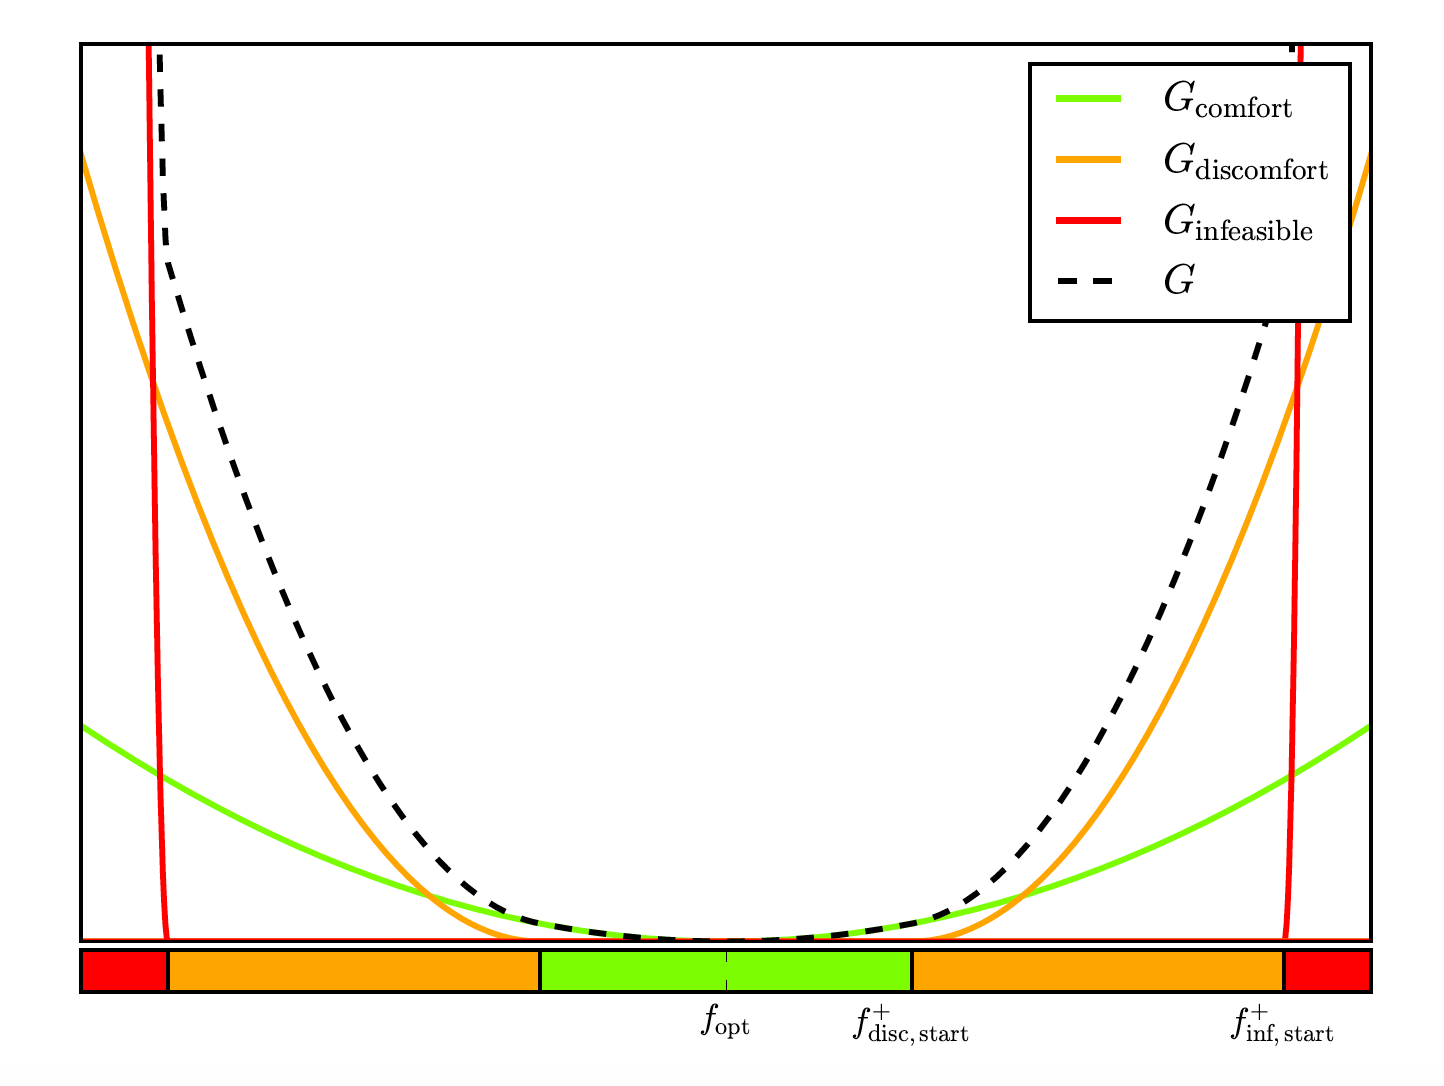
\includegraphics[width = 0.5 \textwidth ]{Kostenfuntion.png}
    \caption[Kostenfunktion]{Darstellung der Kostenfunktion}
    \label{fig:Kostenfuntion}
 \end{figure}


\subsection{Samplingbasiertes L\"osungsverfahren}
\label{sec:SmapPVD}
Wie bereits in Kapitel~\ref{globaleLV} erw\"ahnt bringt eine kooperative Trajektorienplanung meist ein nicht konvexes Optimierungsproblem mit sich.
Ein lokales L\"osungsverfahren k\"onnte nur bei einer starken Vereinfachung des Optimierungsproblems angewandet werden.
Es wird deshalb auf ein globales, samplingbasiertes L\"osungsverfahren zur\"uckgegriffen.
Da ein solches randomisiertes L\"osungsverfahren vergleichsweise uneffizient ist m\"ussen vereinfachende Annahmen getroffen werden, um das Ziel eines echtzeitf\"ahigen Algorithmus erreichbar zu machen.
Wie unter anderem in \cite{Ziegler2017}, \cite{Werling2011} und \cite{Rathgeber2016} kann sich auch hier zu Nutze gemacht werden, dass durch die Stra{\ss}e eine hochstrukturierte Umgebung gegeben ist.
Der Fahrkorridor ist dadurch weitestgehend eingeschr\"ankt.
In diesem Fall wird sich dies zu Nutze gemacht, indem auf die in \cite{Kant1986} vorgestellte \gls{pvd} zur\"urck gegriffen wird.
Hier findet die Trajektorienplanung in zwei separaten Schritten statt:

\begin{enumerate}
\item Generierung eines geometrischen Pfades der eine Kollision mit statischen Objekten vermeidet.
\item Generierung eines Geschwindigkeitsprofils f\"ur den gegebenen Pfad, sodass eine Kollision mit dynamischen Hindernissen vermieden wird.
\end{enumerate}

Der Pfad kann in vielen F\"allen als gegeben angenommen werden.
Eingeschr\"ankt durch die Fahrbahnmakierungen ergibt er sich oft durch die Fahrstreifenmitte. 
Soll nicht die Fahrstreifenmitte als Pfad angenommen werden kann auf bew\"ahrte Verfahren der Pfadgenerierung zur\"uck gegriffen werden.

Ist der Pfad bereits gegeben muss nun noch das Geschwindigkeitsprofil ermittelt werden.
Es ergibt sich somit eine eindimensionale Kontrollvariable.
Dadurch ist das Optimierungsproblem gut geeignet f\"ur ein Samplingverfahren.
Daf\"ur wird die gesuchten Trajektorien \gls{symb:x_optTra}(t) durch equidistante Zeitschritte diskretisiert:

\begin{equation}
\pmb{x}_k=\pmb{x}(t_k),   \quad t_k =t_0+k h
\end{equation}

mit der Diskretisierungsschrittweite \gls{symb:h}.
Um eine Trajektorie zu generieren wird nun f\"ur jeden Zeitschritt ein willk\"urlicher Ruck generiert.
Der Ruck ist die Ableitung der Beschleunigung.
Durch numerische Integration mittels des Finite"=Differenzen"=Verfahrens wird nun f\"ur jeden einzelnen Zeitschritt die Beschleunigung, Geschwindigkeit und die zur\"uckgelegte Wegstrecke entlang des Pfades berechnet werden.
Der Anfangszustand ist durch die Startbeschleunigung, -geschwindigkeit und -position gegeben.
Dieses Vorgehen ist in Abbildung~\ref{fig:Sampling} illustriert.
Zusammen mit dem im vorausgehenden Schritt generierten Pfad ergeben sich nun die Positionen \gls{symb:x_TraDisk} \( = (x_k, y_k)^T\) des Fahrzeuges an den einzelnen Zeitschritten und schlie{\ss}lich durch Interpolation zwischen den Zeitschritten die gesuchte Trajektorie \gls{symb:x_optTra}(t)\(= (x(t), y(t))^T\).

\begin{figure}[!htbp]
    \centering
    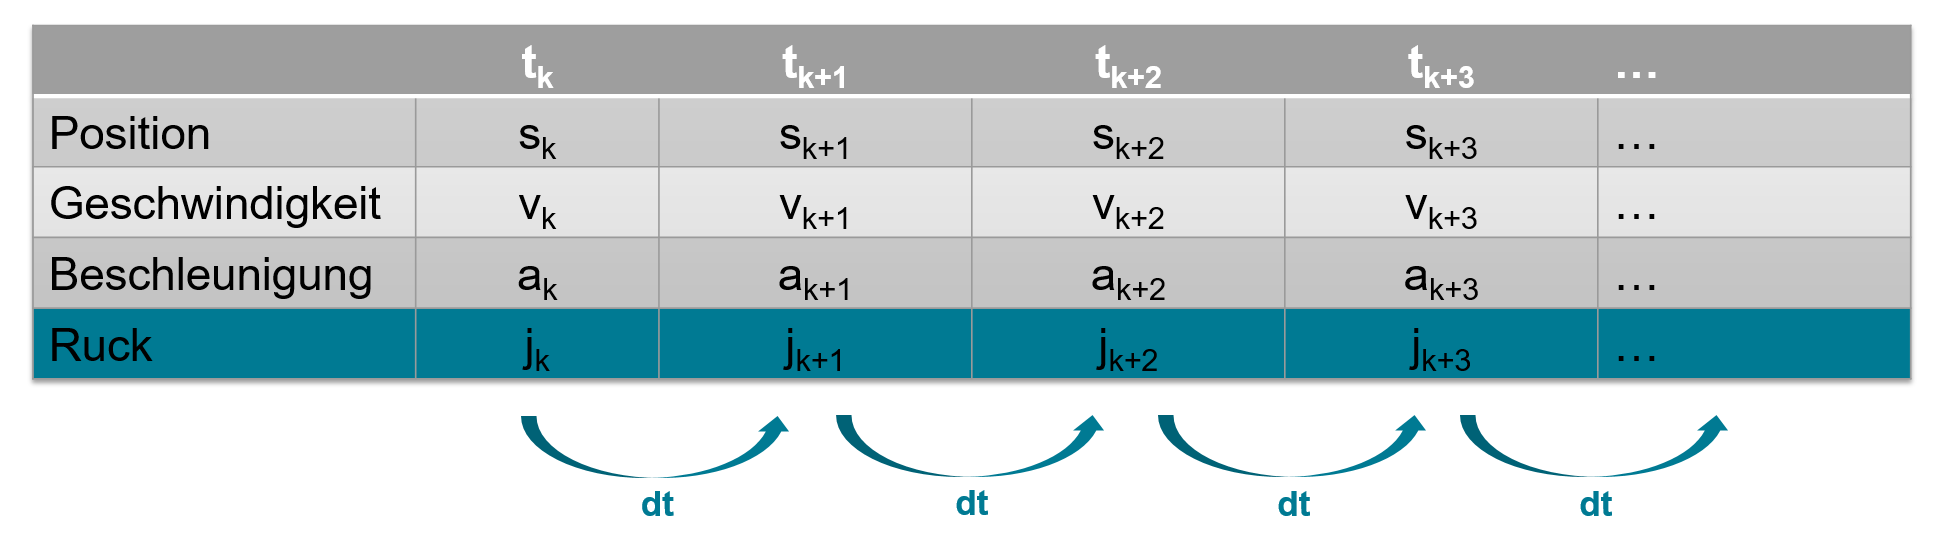
\includegraphics[width = 0.9 \textwidth ]{Sampling.png}
    \caption[Sampling]{Erzeugung eines Geschwindgkeitsprofils \"uber gesampelten Rucken}
    \label{fig:Sampling}
 \end{figure}

F\"ur jedes der beteiligten Fahrzeuge wird eine Vielzahl von Geschwindigkeitsprofilen und somit auch Trajektorien generiert.
Im Anschluss werden alle m\"oglichen Trajektorienkombinationen anhand des in Kapitel~\ref{sec:Kostfunc} vorgestellten Kostenfunktionals bewertet.
Die Trajektorienkombination mit den geringsten Kosten ergibt die angen\"aherte L\"osung des Multi"=Agenten"=Optimimierungsproblems.

Der Ruck wird zuf\"allig aus einem Wertebereich ermittelt, der durch einen vorgegeben maximalen und minimalen Ruck begrenzt ist.
Dadurch kann sicher gestellt werden, dass nur R\"ucke erzeugt werden die als komfortable empfunden werden.
Innere Nebenbedingungen wie maximal zul\"assige Geschwindigkeiten oder Beschleunigungen werden ber\"ucksichtigt, indem der zul\"assige Berreich des Rucks noch weiter eingeschr\"ankt wird.
Dazu wird der maximale bzw. minimale Ruck berechnet, der zul\"assig ist ohne im darauf folgenden Zeitschritt einen Grenzwert zu \"uberschreiten.
Wird beispielsweise bereits mit der maximalen Beschleunigung beschleunigt, darf der Ruck in diesem Zeitschritt den Wert \(0\) nicht \"ubersteigen, womit die maximale Beschleunigung nicht \"uberschritten werden kann.
Analog wird bei Geschwindigkeitsgrenzwerten vorgegangen.


% \subsection{Sicherheitsbetrachtungen}


\section{Bedingungen und Annahmen}

In diesem Abschnitt werden Bedingungen und Annahmen, die dem in dieser Arbeit entwickelten Ansatz zur kooperativen Trajektorienplanung von Fahrstreifenwechseln zu Grunde liegen, vorgestellt.
Auch auf die Einschr\"ankungen die sich dadurch Ergeben wird teilweise eingegangen.

In Kapitel~\ref{Einordung_Trajktorieplanung} wurde gezeigt, dass das Planungsmodul zwischen dem Wahrnehmungsmodul und dem Regelungsmodul eingeordnet werden kann.
Der Fokus dieser Arbeit liegt auf dem Planungsmodul und hier bei im Speziellen auf der Trajektorienplanung.
Aus diesem Grund soll die vereinfachende Annahme getroffen werden, dass das Planungsmodul die Information von einem perfekten Wahrnehmungsmodul erh\"alt und die auszuf\"uhrende Trajektorie an ein perfektes Regelungsmodul weiter gibt.
In der praktischen Anwendung erh\"alt das Planungsmodul vom Wahrnehmungsmodul ein Lagebild der Fahrzeugumgebung.
Dabei handelt es sich um eine unvollst\"andige Sch\"atzung.
In dieser Arbeit soll hingegen davon ausgegangen werden, dass sowohl die Zust\"ande als auch die Abma{\ss}e der erfassten Objekte vollst\"andig durch das Wahrnehmungsmodul bekannt sind.
Die vom Planungsmodul generierte Trajektorie wird dann an das Regelungsmodul weitergegeben.
Die Aufgabe des Regelungsmoduls ist es, das Fahrzeug entlang der vorgegeben Trajektorie zu f\"uhren bis eine neue Trajektorie vorgegeben wird.
Dabei m\"ussen \"au{\ss}ere St\"oreinfl\"usse und Ungenauigkeiten der Aktuatorik ausgeglichen werden.
Dadurch bedingt folgt das Fahrzeug nicht exakt der vorgegebenen Trajektorie.
In dieser Arbeit wird davon ausgegangen, dass die Abweichungen vernachl\"assigbar sind.
Damit entspricht die gefahrene Trajektorie der geplanten Trajektorie und es kann davon ausgegangen werden, dass die geplante Trajektorie aus dem vorherigen Planungsschritt fehlerfrei als Ausgangspunkt f\"ur den aktuellen Planungsschritt genutzt werden kann.
 
Ebenfalls in Kapitel~\ref{Einordung_Trajktorieplanung} wurde erl\"autert, dass f\"ur das Wahrnehmungsmodul ein kartenbasierter oder ein rein sensorischer Ansatz gew\"ahlt werden kann.
Ein rein sensorische Ansatz hat den Vorteil, dass er unsensibel gegen\"uber Ver\"anderung der als statisch angenommenen Umgebung ist.
Jedoch stellt er hohe Anforderungen an das Wahrnehmungsmodul.
H\"aufig kann das vorhandene Wahrnehmungsmodul den hohen Anforderungen nicht gerecht werden.
Aus diesem Grund beruhen viele vollautomatisierte Fahrsysteme auf einem kartenbasierten Wahrnehmungsmodul.
Auch in dieser Arbeit soll von einem kartenbasierten Wahrnehmungsmodul ausgegangen werden.
Dabei wird davon ausgegangen, dass alle Fahrstreifenverl\"aufe und Fahrbahnmarkierungen in der Karte hinterlegt sind.
Es wird au{\ss}erdem davon ausgegangen das Information wie die fr\"uhste und sp\"ateste M\"oglichkeit eines Fahrstreifenwechsels durch die Karte gegeben sind.

In vielen Fahrsituation ist nicht eindeutig zu sagen, welche Route ein anderes Fahrzeug fahren wird.
So kann beispielsweise an einer Kreuzung nicht zweifelsfrei bestimmt werden ob das andere Fahrzeug geradeaus fahren wird oder abbiegen wird.
Selbst wenn der Fahrrichtungsanzeiger (Blinker) verwendet wurde ist es nicht sicher, dass sich das Fahrzeug auch daran halten wird.
In manchen Situationen ist zwar die Route des Fahrzeuges bekannt, aber es ist schwer vorauszusagen ob bzw. wann ein Fahrzeug den Fahrstreifenwechsel durchf\"uhren wird.
Diese Unsicherheiten erfordern ein komplexes Pr\"adiktionsmodell.
In dieser Arbeit soll davon ausgegangen werden, dass alle Fahrzeuge, bis auf das Ego"=Fahrzeug, ihrem aktuellem Fahrstreifen folgen.
Damit sind sowohl die Route als auch der Pfad aller anderen Fahrzeuge bekannt.
Es kann auf eine einfachere fahrstreifenbasierte Pr\"aditkion zur\"uckgegriffen werden.
In vielen praktischen Anwendungen m\"usste dieses durch ein komplexeres Pr\"adiktionsmodell ersetzt werden.

Wie in Kapitel~\ref{sec:Neuplanung} beschrieben, erfordern zahlreiche Unsicherheiten in der Planung eine fortlaufende Neuplanung.
Damit so schnell wie m\"oglich auf die sich neu ergebende Situation reagiert werden kann, sollte die Zeit zwischen zwei Planungsschritten m\"oglichst kurz gehalten werden.
In der Regel ist die Zeit zwischen zwei Planungschritten festgelegt.
F\"ur die Anwendung im realen Verkehr muss deshalb garantiert werden, das ein Planungsschritt in weniger als dieser Zeit durchgef\"uhrt werden kann.
Ziel dieser Arbeit ist es einen Ansatz zu entwickeln, der in der Simulation getestet werden kann.
Die Echtzeitf\"ahigkeit des Algorithmus wird deshalb nicht gefordert.
Es wird bei der Entwicklung des Ansatzes jedoch darauf geachtet, dass bei steigender Anzahl an betrachteten Fahrzeuge die Rechenzeit moderat steigt, sodass auch eine Anwendung im dichten Verkehr plausible bleibt. 		
% !TeX root = ../thesis.tex

\chapter{Ansatz}
\label{sec:concepts}
Ein Fahrstreifenwechsel ist ein h\"aufig angewendetes Fahrman\"over das aus verschieden Gr\"unden durchgef\"uhrt wird.
So kann ein Fahrstreifenwechsel notwendig sein um einer vorgegebenen Route zu folgen oder er wird durchgef\"uhrt um ein langsameres Fahrzeug zu \"uberholen.
Da ein Fahrstreifenwechsel von mehreren Verkehrsteilnehmern gleichzeitig abh\"angt ist er ein komplexes Fahrman\"over \cite{Gipps1986}.
Dies gilt vor allem bei dichtem Verkehr.
F\"ur einen erfolgreichen und sicheren Fahrstreifenwechsel in dichtem Verkehr sind sowohl taktische Entscheidungen (\cite{Ulbrich2015towards}) als auch ein kooperatives Verhalten (\cite{Wei2013}) notwendig.

In diesem Kapitel wird ein Ansatz f\"ur die Trajektorienplanung eines kooperativen Fahrstreifenwechsel von hochautomatisierten Fahrzeugen vorgestellt.
Der Fahrstreifenwechsel findet in Interaktion mit nicht automatisierten Fahrzeugen statt.
Dazu soll zun\"achst die Auswahl des Basisalgorithmus begr\"undet werden.
In diesem Zuge wird auf einige Grundlagen zum Thema Fahrstreifenwechsel eingegangen.
Anschlie{\ss}end werden die Einschr\"ankungen, die sich durch den Basisalgorithmus ergeben, beschrieben.
Aus den Einschr\"ankungen l\"asst sich ableiten welche Anpassungen des Basisalgorithmus f\"ur die Anwendung bei einen Fahrstreifenwechsel notwendig sind.
Basierend darauf wird der Ansatz f\"ur einen einzelnen Planungsschritt vorgestellt.
Aufgrund von Unsicherheiten unterschiedlicher Art in der Planung muss dieser Planungsschritt in regelm\"a{\ss}igen zeitlichen Abst\"anden wiederholt werden.
Auf diesen Aspekt wird in Kapitel~\ref{sec:Neuplanung} eingegangen.

\section{Auswahl und Einschr\"ankungen des Basisalgorithmus}
In diesem Abschnitt wird zun\"achst die Auswahl Basisalgorithmus begr\"undet.
In dieser Arbeit wurde der von Naumann und Stiller \cite{Naumann2017towards} vorgestellte Ansatz f\"ur eine kooperative Bewegungsplanung als Basisalgorithmus ausgw\"ahlt. 
Zur Begr\"undung der Auswahl wird auf einige grundlegende Aspekte eines Fahrstreifenwechsels eingegangen.
Aus dem Basisalgorithmus ergeben sich Einschr\"ankungen die daf\"ur sorgen, dass er nicht direkt auf einen Fahrstreifenwechsel anwendbar ist.
Diese sollen anschlie{\ss}end herrausgearbeitet werden.
Aus den sich ergebenden Einschr\"ankungen l\"asst sich schlie{\ss}en, welche Anpassungen notwendig sind um den Ansatz der kooperativen Bewegungsplanung auf eine Fahrstreifenwechsel anzuwenden. 

\subsection{Auswahl des Basisalgorithmus}
\label{sec:AuswahlBA}
Fahrstreifenwechsel sind gebr\"auchliche Fahrman\"over in allt\"aglichen Fahrsituationen.
Die Gr\"unde aus denen ein Fahrstreifenwechsel ausgef\"uhrt wird sind unterscheidlich.
In der Literatur wird h\"aufig zwischen zwingend notwendigen (englisch: mandatory) und frei verf\"ugbaren (englisch: discretionary) Fahrstreifenwechseln unterschieden (\cite{Toledo2003}, \cite{Yang1996}).
Ein Fahrstreifenwechsel ist zwingend notwendig, wenn der aktuelle Fahrstreifen endet oder um einer vorgegebenen Route zu folgen.
Frei verf\"ugbare Fahrstreifenwechsel werden in erster Linie angewandt um langsamere Fahrzeuge zu \"uberholen.

Ein Fahrstreifenwechsel stellt ein vergleichsweise komplexes Fahrman\"over dar, das gro{\ss}es Potential f\"ur Sicherheitsrisiken birgt und direkten Einfluss auf den Verkehrsfluss hat \cite{Julian2015}.
Bei dichtem Verkehr muss in der Planung die Interaktion mit anderen Fahrzeugen ber\"ucksichtigt werden \cite{Hubmann2018}.
Es muss ein Kompromiss zwischen den eigenen Vorteilen und den Nachteilen anderer Verkehrsteilnehmer gefunden werden \cite{Kesting2007}.
Laut Gipps \cite{Gipps1986} m\"ussen folgende taktische Entscheidungen getroffen werden: 

\begin{itemize}
\item Ist ein Fahrstreifenwechsel m\"oglich
\item Ist ein Fahrstreifenwechsel notwendig
\item Ist ein Fahrstreifenwechsel w\"unschenswert
\end{itemize}


Viele existierende Ans\"atze unterteilen das Planungsproblem f\"ur einen Fahrstreifenwechsel in mehrere Teilprobleme. 
Zu den Teilproblemen geh\"ort die L\"uckenauswahl, die Ann\"aherung an die L\"ucke, die Bewertung der L\"ucke und das Einf\"adeln in die L\"ucke.
Diese Teilprobleme werden getrennt voneinander gel\"ost. \cite{Hubmann2018}
Laut Hubmann et al. \cite{Hubmann2018} ist dadurch zwar eine vereinfachte, hierachische Problemformulierung m\"oglich, es wird jedoch gleichzeitig der Raum m\"oglicher L\"osung reduziert.
Dies kann dazu f\"uhren, dass bei dichtem Verkehr keine L\"osung gefunden werden kann.
Handelt es sich um einen notwendigen Fahrstreifenwechsel bedeutet dies, dass das Fahrzeug auf dem aktuellen Fahrstreifen zum Stehen kommt bis sich eine L\"ucke bietet, die gro{\ss} genug ist, um den Fahrstreifenwechsel sicher ausf\"uhren zu k\"onnen.
Dies erschwert den Fahrstreifenwechsel noch weiter und birgt au{\ss}erdem hohe Sicherheitsrisiken und sollte deshalb m\"oglichst vermieden werden.

Menschlich gef\"uhrten Fahrzeugen gelingt ein Fahrstreifenwechsel in der Regel auch in dichtem Verkehr.
Dies liegt dran, dass sie in vielen F\"allen sowohl kooperatives Verhalten gegen\"uber anderen Fahrzeuge zeigen als auch kooperatives Verhalten von anderen Fahrzeugen erwarten.
Ein solches Verhalten ist m\"oglich, weil Menschen in der Regel die Intentionen anderer Fahrzeuge einsch\"atzen k\"onnen und entsprechend darauf reagieren.
Bei einem Fahrstreifenwechsel k\"onnen die Fahrzeuge auf dem Zielfahrstreifen auf unterschiedliche Arten ein kooperatives Verhalten zeigen.
Sie k\"onnen ihre Geschwindigkeit leicht erh\"ohen oder verringern um die L\"ucke f\"ur das auffahrende Fahrzeuge zu vergr\"o{\ss}ern.
Oder sie machen ebenfalls einen Fahrstreifenwechsel auf einen dritten Fahrstreifen und machen so eine L\"ucke auf dem Zielfahrstreifen des Ego"=Fahrzeuges auf.
Automatisierte Fahrzeug, die nicht \"uber ein kooperatives Verhalten verf\"ugen, zeigen in solchen Situationen h\"aufig ein Verhalten das als sozial nicht akzeptabel beschrieben werden kann.
Das f\"uhrt dazu, dass es f\"ur menschliche Fahrer schwer wird automatisierte Fahrzeuge einzusch\"atzen und k\"onnte zu gef\"ahrlichen Situationen f\"uhren. \cite{Wei2013}

Aus diesem Grund sollten f\"ur einen Fahrstreifenwechsel bei dichtem Verkehr ein kooperativer Planungsansatz mit interaktionsbewusster Bewegungspr\"adiktion verwendet werden.
In Wei et al. \cite{Wei2013} konnte durch einen Ansatz der ein soziales, kooperatives Fahrverhalten ber\"ucksichtigt die Kosten f\"ur einen Fahrstreifenwechsel um 41.7 \% reduziert werden.
Der Vergleich fand aufgrund eines ausgew\"ahlten Kostenfunktionals statt.
Eine Planung in der die Interaktion mit anderen Fahrzeugen ber\"ucksichtigt wird f\"uhrt jedoch dazu, dass die Bewegungspr\"adiktion anderer Fahrzeuge nicht mehr entkoppelt von der Trajektorienplanung stattfinden kann \cite{Hubmann2018}.
Es muss also ein Ansatz gew\"ahlt werden, bei der die Bewegungspr\"aditktion in die Bewegungsplanung integriert wird.

Diese M\"oglichkeit bietet der von Naumann und Stiller \cite{Naumann2017towards} vorgestellte Ansatz einer Mulit"=Agenten"=Optimierung.
Durch die Verwendung eines Kostenfunktionals, das die Gesamtkosten aller Fahrzeuge ber\"ucksichtigt, wird von einem kooperativen Verhalten aller Fahrzeuge ausgegangen.
Der Ansatz bietet au{\ss}erdem die M\"oglichkeit ebenfalls die Man\"overplanung in die Bewegungsplanung zu integrieren.
Er wurde deshalb als Basisalgorithmus ausgew\"ahlt.
Es ergeben sich jedoch Einschr\"ankungen die eine Anpassung f\"ur die Anwendung auf einen Fahrstreifenwechsel notwendig machen.
Diese werden im n\"achsten Abschnitt erl\"autert.


\subsection{Einschr\"ankungen des Basisalgorithums}
\label{Grenzen}
Der von Naumann und Stiller \cite{Naumann2017towards} vorgestellte Ansatz zur kooperativen Trajektorienplanung, der hier als Basisalgorithmus bezeichnet wird, wurde bereits simulativ in zwei Verkehrszenarien validiert.
Diese zwei Verkehrszenarien stellen zwei typische Situationen dar, in den \"ublicherweise kooperatives Verhalten gefordert ist.
In einer ersten Simulation wurde der Ansatz f\"ur eine Trajektorienplanung an einer ungeregelten Engstelle (siehe Abbildung~\ref{fig:Engstelle}) validiert.
Hier steht zwei entgegengerichteten Fahrrichtungen f\"ur einen kurzen Abschnitt lediglich eine gemeinsame Spur zur Verf\"ugung.
Die Fahrzeuge m\"ussen entscheiden welches zuerst in die Engstelle einf\"ahrt und welches das andere Fahrzeug passieren lassen muss.
Bei einem rein reaktiven Ansatz bei dem beide Fahrzeuge davon ausgehen, dass das jeweils anderen Fahrzeug zuerst einf\"ahrt, kann dies zu einer Patt"=Situationen f\"uhren in der beide Fahrzeuge zum Stillstand kommen.
In einem zweiten Szenario wurde das Linksabbiegen an einer T-Kreuzung simuliert (siehe Abbildung~\ref{fig:Kreuzung}).
In dieser Situation muss das Ego"=Fahrzeug aufgrund des Kostenfunktionals entscheiden, ob es vor oder nach dem entgegenkommenden Fahrzeug abbiegen soll.
Die beiden Szenarien sind in Abbildung~\ref{fig:SimSzen} dargestellt.

\begin{figure}[!htbp]
    \centering
    \subfigure[Engstelle ohne Vorfahrtsregelung \cite{Naumann2017towards}]{
        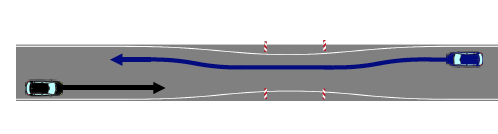
\includegraphics[width = 0.55 \textwidth]{Engstelle.png}
        \label{fig:Engstelle}
    }
    \hfill
     %add desired spacing between images, e. g. ~, \quad, \qquad, \hfill etc.
     %(or a blank line to force the subfigure onto a new line)
    \subfigure[Linksabbiegen an einer T-Kreuzung  \cite{Naumann2017towards}]{
        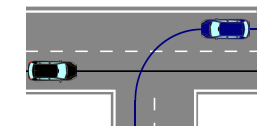
\includegraphics[width = 0.35  \textwidth]{Kreuzung.png}
        \label{fig:Kreuzung}
    }
    \caption[Anpassung f\"ur globales Minimum]{Simulierte Szenarien des Basisalgorithmus}
    \label{fig:SimSzen}
\end{figure}

Anhand der Simulationen konnte gezeigt werden, dass es dem Ansatz des Basisalgotihmus in beiden Szenarien m\"oglich ist sichere, komfortabel und kooperative Trajektorien zu generieren.
Auch ohne eine sogenannte Fahrzeug"=zu"=Fahrzeug Kommunikation konnte mit anderen Fahrzeugen kooperiert werden und damit eine vorteilhafte L\"osung gefunden werden.
In beiden F\"allen konnten die Pfade der beteiligten Fahrzeuge als durch den Streckenverlauf gegeben angenommen werden.
Zur Generierung von m\"oglichen Trajektorien mussten deshalb nur noch verschiedene Geschwindigkeitsprofile erzeugt werden.
Die in Kapitel~\ref{sec:SmapPVD} beschriebene Path"=Velocity"=Decomposition \gls{pvd} ist somit direkt anwendbar.
F\"ur beide Fahrzeuge wurde nun eine Vielzahl von zuf\"alligen Trajektorien generiert und anschlie{\ss}end alle sich ergebenden Kombinationen anhand eines Kostenfunktionals bewertet.

Wird nun ein Fahrstreifenwechsel betrachtet werden die Einschr\"ankungen des Basisalgorithmus offensichtlich.
Zum einen ist der Pfad bei einem Fahrstreifenwechsel nicht mehr komplett durch den Stra{\ss}enverlauf vorgegeben.
In vielen F\"allen ist nicht vorgegeben wann bzw. wo der Fahrstreifenwechsel eingeleitet werden soll.
Bei einem \"Uberholman\"over auf einer mehrspurigen Fahrbahn sollte der Fahrstreifenwechsel zum \"Uberholen eines langsameren Fahrzeuges eingeleitet werden bevor es zu Unterschreitung von Sicherheitsabst\"anden kommt.
Auf einer Beschleunigungsspur sollte der Fahrstreifenwechsel eingeleitet werden sobald sich eine L\"ucke ergibt die gro{\ss} genug ist.
Der zu fahrende Pfad h\"angt damit stark vom Geschwindigkeitsprofil des Fahrzeuges ab.
Die Ermittlung von Pfad und Geschwindigkeitsprofil kann also nicht entkoppelt voneinander stattfinden.
Ein Ausnahme bilden Einf\"adelszenarien bei denen sich die Fahrzeuge nach dem Rei{\ss}verschlussverfahren auf dem neuen Fahrstreifen einordnen sollen.
Hier ist vorgegeben, dass der Fahrstreifenwechsel am Fahrstreifenende stattfinden soll.
Doch auch hier h\"angt der geometrische Pfad des Fahrstreifenwechsels von der Geschwindigkeit des Fahrzeuges ab.
F\"ahrt das Fahrzeug vergleichsweise langsam, so kann der Fahrstreifenwechsel auf einer relativ kurzen Strecke statt finden.
Bei h\"oheren Geschwindigkeiten w\"urden bei dem selben Pfad die Kr\"ummung des Pfades zu hohen Querbeschleunigungen f\"uhren.
Der Fahrstreifenwechsel muss also auf einer l\"angeren Strecke stattfinden.
Die vorgestellte \gls{pvd} ist somit nicht mehr direkt anwendbar.
Es gilt den Pfad in Abh\"angigkeit vom eigenen Geschwindigkeitsprofil zu generieren.
Gegebenenfalls sollten bei der Pfadplanung auch dynamische Hindernisse, mit denen keine direkte Interaktion stattfindet, in Betracht gezogen werden.

Ein weiterer Nachteil ist, dass der Rechenaufwand f\"ur einen einzelnen Planungsschritt stark von der Anzahl der in Betracht gezogenen Fahrzeuge abh\"angt.
Nehmen wir ein Szenario an, in dem lediglich ein anderes Fahrzeug f\"ur eine Kooperation in Frage kommt.
Dies ist in den beiden simulierten Szenarien der Fall.
Au{\ss}erdem sollen f\"ur jedes der Fahrzeuge 1000 Trajektorien generiert werden.
So ergeben sich \( 10^6 \) m\"ogliche Trajektorienkombinationen.
Kommt ein weiteres Fahrzeug hinzu ergeben sich bereits \( 10^9 \) m\"ogliche Trajektorienkombinationen.
Die Anzahl der zu bewertenden Trajektorienkombinationen steigt mit jedem weiteren Fahrzeug stark an.
Kooperative Ans\"atze f\"ur einen Fahrstreifenwechsel zeigen vor allem dann ihr Vorteile gegen\"uber reaktiven Ans\"atzen, wenn der Zielfahrstreifen dicht befahren ist.
Bei einem dicht befahrenen Zielfahrstreifen kommen jedoch mehrere Fahrzeuge f\"ur eine Kooperation in Frage.
Werden nun die Kombinationen aller in Frage kommender Fahrzeuge bewertet, steigt der Rechenaufwand schnell stark an.
Dies wirkt der gew\"unschten Echtzeitf\"ahigkeit des Algorithmus entgegen.


\section{Planungschritt}
In Kapitel~\ref{Grenzen} wurden die Einschr\"ankungen des Basisalgorithmus beschrieben.
Diese machen eine Anpassung des Algorithmus notwendig, um ihn f\"ur einen Fahrstreifenwechsel anzuwenden.
Zum einen steigt bei Ber\"ucksichtigung mehrerer Fahrzeuge die Laufzeit des Algorithmus stark an.
Zum anderen kann bei der Planung eines Fahrstreifenwechsels die Pfadplanung nicht mehr entkoppelt von der Ermittlung des Geschwindigkeitsprofils statt finden.

Ist bereits die Fahrstreifenwechseltrajektorie des Ego"=Fahrzeuges bekannt, kann die Anzahl der m\"oglichen kooperativen Partner stark eingeschr\"ankt werden.
Wird von einem einzelnen Fahrstreifenwechsel ausgegangen und die Annahme getroffen, dass kein anderes Fahrzeug den Fahrstreifen wechselt, h\"angt der Fahrstreifenwechsel von nur vier Fahrzeugen ab.
Dem vorausfahrendem und folgenden Fahrzeug auf dem aktuellem Fahrstreifen und dem vorausfahrendem und folgenden Fahrzeug auf dem Zielfahrstreifen.
Die Trajektorie f\"ur den Fahrstreifenwechsel kann weitestgehend unabh\"angig vom Folgefahrzeug des akutellen Fahrstreifens geplant werden, da es in dessen Verantwortung ist den n\"otigen Sicherheitsabstand einzuhalten.
Es sollten lediglich unerwartet starke Verz\"ogerungen vermieden werden.
Zum vorausfahrenden Fahrzeug auf des aktuellen Fahrstreifens gilt es selbst f\"ur einen ausreichenden Sicherheitsabstand zu sorgen.
Hier ist ein reaktives Fahrverhalten ausreichend.
F\"ur eine Kooperation kommen somit nur noch das vorausfahrende und das folgende Fahrzeug auf dem Zielfahrstreifen in Frage.
Diese k\"onnen durch Anpassung ihres eigenen Geschwindigkeitsprofils daf\"ur sorgen, dass dem Ego"=Fahrzeug das Auffahren auf den Zielfahrstreifen erleichtert wird.

Die Begrenzung auf maximal zwei kooperierende Fahrzeuge pro Fahrstreifenwechsel wird sich bei dem nun vorgestellten Ansatz zur kooperativen Fahrstreifenwechseltrajektorienplanung zu Nutze gemacht werden.
Es wird nun nicht f\"ur alle m\"oglichen Kandidaten eine Vielzahl von zuf\"alligen Geschwindigkeitsprofilen erzeugt, sondern erst einmal nur f\"ur das Ego"=Fahrzeug.
Dabei ist der Pfad des Ego"=Fahrzeuges zun\"achst noch unbekannt.
Zus\"atzlich findet eine Bewegungspr\"adiktion aller relevanten Fahrzeuge in der Umgebung des Ego"=Fahrzeuges statt.
Diese Pr\"adiktion ist vorerst unabh\"angig vom Ego"=Fahrzeug.

Nun wird f\"ur jedes erzeugte Geschwindigkeitsprofil ein Pfad generiert.
Um m\"oglichst viele valide Trajektorien zu generieren k\"onnen hier gegebenfalls Information aus der Bewegungspr\"adiktion genutzt.
In der Pfadplanung werden sowohl die geometrischen Punkte bestimmt an denen der Fahrstreifenwechsel beginnen und enden soll, als auch die geometrische Verbindung dieser Punkte.
Ist sowohl das Geschwindigkeitsprofil als auch der Pfad des Ego"=Fahrzeuges gegeben, ergibt sich daraus die diskretisierte Trajektorie des Ego"=Fahrzeuges.
Anhand dieser Trajektorie und der vom Ego"=Fahrzeug unabh\"angigen Bewegungspr\"adiktion k\"onnen nun m\"oglich kooperative Partner bestimmt werden.
Dies findet im sogenannten Klassifizierungsschritt statt.

In einer inneren Optimierung wird dann f\"ur diese Fahrzeuge eine kooperative Trajektorie bestimmt. 
Zur L\"osung des inneren Optimierungsproblems wird auf das samplingbasierte L\"osungsverfahren des Basisalgorithmus zur\"uckgegriffen, wobei jedoch die Trajektorie des Ego"=Fahrzeuges fest vorgegeben ist.
Sind nun die Trajektorien der kooperativen Fahrzeuge bestimmt, findet darauf beruhend eine neue Bewegungspr\"adiktion aller anderen Fahrzeuge statt.
Soll kein weiterer Fahrstreifenwechsel innerhalb des Planungshorizonts durchgef\"uhrt werden, kann das resultierende Trajektorienset anhand des Kostenfunktionals bewertet werden.
Das Trajektorienset enth\"alt die Trajektorien aller betrachteten Fahrzeuge.
In manchen F\"allen, wie zum Beispiel dem \"Uberholen mit Gegenverkehr, ist es jedoch wichtig, dass auch ein zweiter Fahrstreifenwechsel geplant wird.
In solchen F\"allen wird vorgeschlagen auf Basis der bisherigen L\"osung die Schritte von der Pfadplanung bis zur Neupr\"adiktion zu wiederholen und anschlie{\ss}end die Bewertung vorzunehmen.

Dieses Vorgehen findet f\"ur alle generierten Geschwindigkeitsprofile statt.
Somit ergibt sich ein Trajektorienset f\"ur jedes Geschwindigkeitsprofil.
Zur Generierung jedes dieser Trajektroiensets muss lediglich f\"ur maximal zwei Fahrzeuge pro Fahrstreifenwechsel eine kooperative Trajektorie bestimmt werden.
Dies ist unabh\"angig davon wie viele Fahrzeug sich in der Umgebung des Ego"=Fahrzeuges befinden.
Der Fahrstreifenwechselpfad wurde aufgrund des gegeben Geschwindigkeitsprofils ermittelt.
Als angen\"aherte L\"osung des \"au{\ss}eren Optimierungsproblems wird nun das Trajektorienset mit den geringsten berechneten Gesamtkosten ausgew\"ahlt.
Die L\"osung enth\"alt auch die Trajektorie des Ego"=Fahrzeuges, die dann an das Regelungsmodul weitergegeben werden kann.
Aufgrund des samplingbasierten Ansatzes ist die Trajektorie allerdings stark diskretisiert.
Falls eine h\"ohere Genauigkeit gefordert ist, wird vorgeschlagen die angen\"aherte L\"osung der Multi"=Agenten"=Optimierung an ein lokales Verfahren zur Trajektoriengenerierung weiterzugegeben.
Beruhend auf dieser L\"osung kann das lokale Verfahren dann eine feiner aufgel\"oste Trajektorie generieren

\begin{figure}[!htbp]
    \centering
    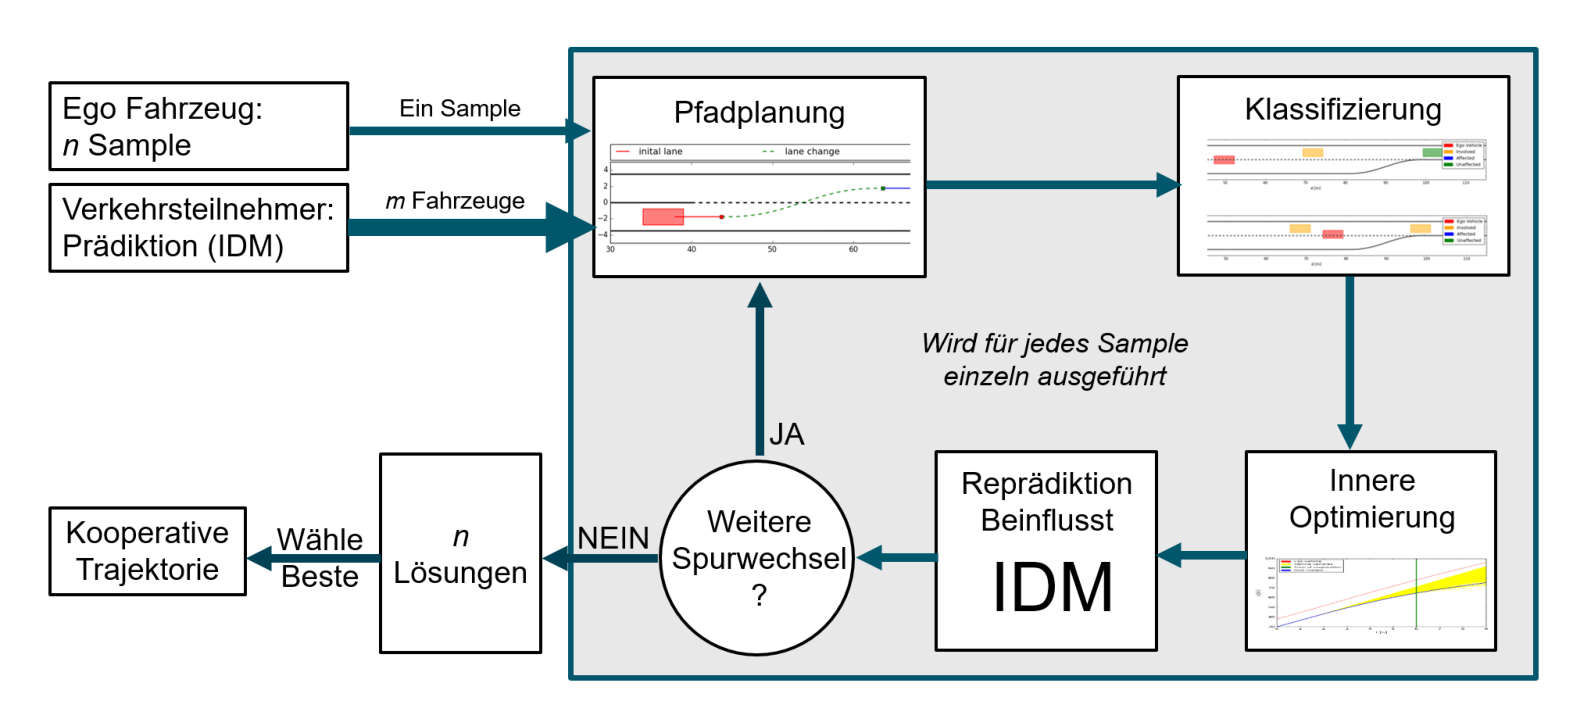
\includegraphics[width = 0.8 \textwidth ]{Ansatz.pdf}
    \caption[Planungsansatz]{Gesamt\"uberblick des Planungsansatzes. \textit{n} steht f\"ur die Anzahl der erzeugten Sample.}
    \label{fig:Ansatz}
 \end{figure}

In Abbildung~\ref{fig:Ansatz} ist ein Gesamt\"uberblick des Ansatzes visualisiert.
Auf wichtige Teilaspekte des Ansatzes wird in den nun folgenden Abschnitten genauer eingegangen.

\FloatBarrier


\subsection{Darstellung in Frenet Koordinaten}
\label{sec:FrenetBesch}
In Kapitel~\ref{sec:Frenet} wurde das Frenet"=Koordinatensystem vorgestellt und seine Verwendung in der Trajektorienplanung dieser Arbeit motiviert.
Eine Beschreibung in Frenet"=Koordinaten entspricht der mathematischen Beschreibung des Stra{\ss}enkoordinatensystems \cite{Rathgeber2016}.
Dabei wird eine Referenzkurve ausgew\"ahlt und die Planung findet dann entlang dieser Referenzkurve statt.
Die Fahrzeugposition wird nun durch die Bogenl\"ange \gls{symb:s_r} entlang der Referenzkurve und den Abstand \gls{symb:d_r} zur Referenzkurve beschrieben.

Es werden mehrere Vorteile genannt die sich durch die Verwendung der Frenet"=Koordinaten ergeben.
Unter anderem wird beschrieben, dass sich durch die Planung in Frenet"=Koordinaten auf einer gekr\"ummten Fahrbahn ein Fahrstreifenwechsel ergibt, der im Vergleich zu einer Planung in Weltkoordinaten mehr einem menschlichen Verhalten entspricht.
Dieser Effekt wird von Werling \cite{Werling2011} beschrieben und soll an dieser Stelle noch einmal genauer erl\"autert werden.

Im realen Verkehr ist h\"aufig ein Fahrstreifenwechsel zu beobachten, der auf gekr\"ummter Fahrbahn im Sinne von Komfort und Effizienz nicht dem Optimum entspricht.
So wird h\"aufig ein in Abbildung~\ref{fig:BeobaSpurwe} dargestellter Fahrstreifenwechsel beobachtet, obwohl der in Abbildung~\ref{fig:OptimalSpurwe} dargestellte Fahrstreifenwechsel aus Komfort- und Effizienzgr\"unden zu bevorzugen w\"are.
Grund daf\"ur ist, dass sich menschliche Fahrer bei der Planung des Fahrstreifenwechsel an den Fahrbahnmarkierungen orientieren.
Diese Planungsstrategie ist in Abbildung~\ref{fig:Planugsstrat} dargestellt.
Eine solche Planungsstrategie erleichtert die Bewegungspr\"adiktion f\"ur die umgebenden Fahrzeuge, da eine Realtivbewegung zur Stra{\ss}e fr\"uher als Absolutbewegung \"uber dem Untergrund wahrgenommen werden kann.
Ein Fahrstreifenwechsel wie in Abbildung~\ref{fig:OptimalSpurwe} dargestellt ist somit f\"ur andere Fahrer schwerer einzusch\"atzen und k\"onnte in dichtem Verkehr zu einer gef\"ahrlichen Situation f\"uhren. 
Deshalb ist auch f\"ur automatisierte Fahrzeuge die in Abbildung~\ref{fig:Planugsstrat} dargestellte Planungstrategie zu bevorzugen.
Eine solche Planungsstrategie ergibt sich, wenn in einer entkr\"ummenten Fahrzeugumgebung geplant wird.
Wie im Kapitel~\ref{sec:Frenet} beschrieben entspricht das einer Planung im Frenet"=Koordinatensystem.
Dies macht deutlich, dass der Pfad des Fahrzeuges in Frenet"=Koordinaten beschrieben werden sollte. \cite{Werling2011}


\begin{figure}[!htbp]
    \centering
    \subfigure[Kostenoptimaler Fahrstreifenwechsel]{
        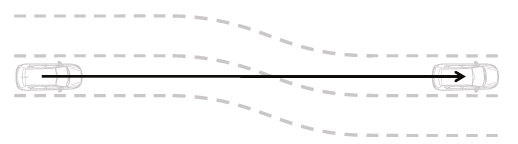
\includegraphics[width = 0.7 \textwidth]{Optimal.png}
        \label{fig:OptimalSpurwe}
    }
    \subfigure[Oft beobachter Fahrstreifenwechsel]{
        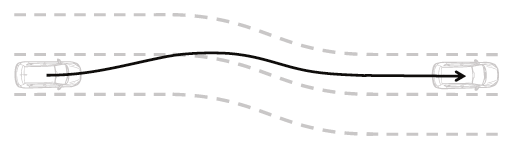
\includegraphics[width = 0.7  \textwidth]{Beobachtet.png}
        \label{fig:BeobaSpurwe}
    }
    \subfigure[Planugsstrategie von oft beobachteten Fahrstreifenwechseln]{
        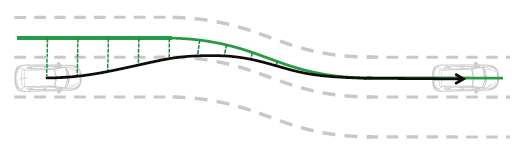
\includegraphics[width = 0.7  \textwidth]{Planungstrategie.png}
        \label{fig:Planugsstrat}
    }
    \caption[Fahrstreifenwechsel in Frenet"=Koordinaten]{Vergleich von unterschiedlichen Fahrstreifenwechselarten. \cite{Werling2011}}
    \label{fig:SimSzen}
\end{figure}


Wie wir in Kapitel~\ref{sec:Pfadplanung} sehen werden, ergibt sich der Pfad f\"ur einen einzelnen Fahrstreifenwechsel immer aus dem Pfad des aktuellen Fahrstreifens, dem Pfad des Zielfahrstreifens und einem verbindenden Zwischenst\"uck.
Zur Beschreibung in Frenet"=Koordinaten muss zus\"atzlich noch eine Referenzkurve gew\"ahlt werden.
Diese sollte m\"oglichst nahe an dem aktuellen Fahrstreifen und dem Zielfahrstreifen sein und au{\ss}erdem einen \"ahnlichen Verlauf haben, da so der Diskretisierungsfehler minimal gehalten werden kann.
Aus diesem Grund wird als Referenzkurve die Fahrbahnmakierung verwendet, die den aktuellen Fahrstreifen vom Zielfahrstreifen trennt.
Bei einem Fahrstreifenwechsel auf den linken Fahrstreifen w\"are dies zum Beispiel die rechte Fahrbahnmarkierung des Zielfahrstreifens.
Da ein doppelter Fahrstreifenwechsel innerhalb von einem Planungsschritt ausgeschlossen wird, sind dies die einzigen Verl\"aufe die zur Fahrstreifenwechselplanung notwendig sind.

Mit einem doppelten Fahrstreifenwechsel sind hierbei zwei Fahrstreifenwechsel in die gleiche Richtung gemeint.
Ein Fahrstreifenwechsel auf den Zielfahrstreifen und wieder zur\"uck auf den Ausgangsfahrstreifen wird dadurch nicht ausgeschlossen.
Dies ist f\"ur die Planung eines Fahrstreifenwechsels mit entgegenkommenden Verkehr wichtig.
Zwei direkt aufeinander folgende Fahrstreifenwechsel k\"onnen in dichtem Verkehr nur selten ausgef\"uhrt werden.
Ein solches Fahrverhalten birgt au{\ss}erdem ein erh\"ohtes Gefahren- und Unfallpotenzial.
Um einen doppelten Fahrstreifenwechsel sicher ausf\"uhren zu k\"onnen muss der Fahrer die Situation auf gleich mehreren Fahrstreifen \"uberblicken.
Zudem ist ein solches Fahrverhalten f\"ur andere Fahrer schwerer einzusch\"atzen.
Deshalb ist es zu bevorzugen zun\"achst einmal einen Fahrstreifenwechsel auszuf\"uhren und sich in den Verkehr des neuen Fahrstreifens einzugliedern.
Ist der Eingliederungsvorgang abgeschlossen kann der n\"achste Fahrstreifenwechsel geplant werden.
Ein solches Verhalten kann durch eine Planung, die zwar einen doppelten Fahrstreifenwechsel ausschlie{\ss}t aber in kurzen Zeitintervallen wiederholt wird, abgebildet werden.
Da eine kontinuierliche Neuplanung ohnehin unabdingbar ist, kann ein doppelter Fahrstreifenwechsel ohne gro{\ss}e Einschr\"ankungen ausgeschlossen werden.

Ist ein Fahrstreifenwechsel durchzuf\"uhren, der aufgrund des Ergebnisses der Routenplanung notwendig ist, sind au{\ss}er den Verl\"aufen der Referenzkurve und der Fahrstreifen noch weitere Informationen notwendig.
So muss bekannt sein bis wann und gegebenfalls auch ab wann ein Fahrstreifenwechsel durchgef\"uhrt werden kann.
Da ein kartenbasierter Ansatz angenommen wird, kann davon ausgegangen werden, dass sowohl diese Informationen als auch die Verl\"aufe der Fahrstreifen und der Referenzkurve gegeben sind.
Gegebenfalls muss noch eine Transformation von Welt- in Frenet"=Koordinaten stattfinden.

Wie in Kapitel~\ref{sec:Frenet} beschrieben erfolgt sowohl die Beschreibung der Fahrzeugeigenbewegung als auch die Beschreibung aller Kraftfahrzeuge in der Umgebung des Ego"=Fahrzeuges in Frenet"=Koordinaten.
Dazu wird die Bewegung der Fahrzeuge auf dem gegeben Pfad entlang der Referenzkurve berechnet.
Die Bewegung entlang der Referenzkurve ergibt sich aus dem Bewegungsanteil in Richtung der Referenzkurve w\"ahrende eines Zeitschrittes.
Bei gekr\"ummter Referenzkurve sollte die Kr\"ummung ebenfalls ber\"ucksichtig werden.
Damit ergibt sich die in Werling \cite{Werling2011} beschriebene Formel zur Berechnung der zur\"uckgelegten Wegstrecke entlang der Referenzkruve:

\begin{equation}
   \dot{s}_r = v \frac{\cos(\theta - \theta_\mathrm{ref})}{1 - d_r \kappa_\mathrm{ref}(s_r)}
\end{equation}

Dabei beschreiben \gls{symb:theta} und \gls{symb:theta_ref}die Richtung der Trajektorie und der Referenzkurve in Weltkoordinaten und \gls{symb:kappa_ref} die Kr\"ummung der Referenzkurve.
Das verwendete Frenet"=Koordinatensystem ist in Abbildung~\ref{fig:Frenet} dargestellt.

\begin{figure}[!htbp]
    \centering
    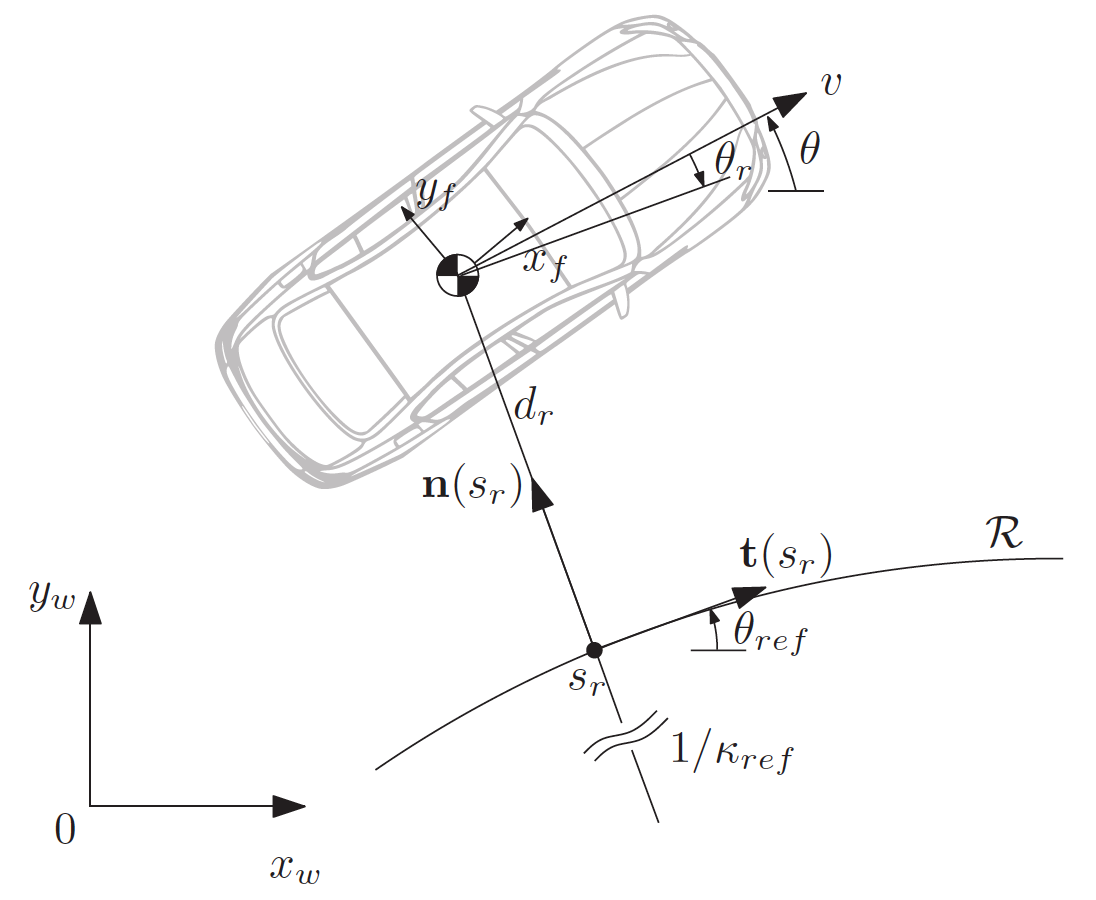
\includegraphics[width = 0.5 \textwidth ]{Frenet.png}
    \caption[Frenet"=Koordinatensystem]{Verwendetes Frenet"=Koordinatensystem \cite{Rathgeber2016}}
    \label{fig:Frenet}
\end{figure}


\FloatBarrier


\subsection{Kostenfunktional}
\label{sec:LCKostfunc}
In Kapitel~\ref{sec:Kostfunc} wird auf das Kostenfunktional des Basisalgorithmus eingegangen.
Dieses ber\"ucksichtigt die Kosten aller relevanten Fahrzeuge f\"ur den kompletten Planungshorizont.
Damit wird ein kooperatives Verhalten aller Verkehrsteilnehmer angenommen.
Es soll nun eine Situation betrachtet werden, in der sich hinter einem Fahrzeug auf dem selben Fahrstreifen ein anderes Fahrzeug befindet das eine h\"ohere Wunschgeschwindigkeit hat.
Durch das Abweichen von dieser Wunschgeschwindigkeit entstehen f\"ur das hintere Fahrzeug Kosten.
Durch das Gesamtkostenfunktional w\"urden sich diese Kosten auch auf das Verhalten des vorausfahrenden Fahrzeuges auswirken und dieses w\"urde wom\"oglich seine Geschwindigkeit erh\"ohen.
Ein solches Verhalten ist zu vermeiden, denn es w\"urde bedeuten, dass auf dr\"angelnde Fahrzeuge reagiert wird.
Dieses Szenario zeigt, dass es f\"ur die Trajektorieplanungen des Ego"=Fahrzeuges nicht sinnvoll ist alle Fahrzeuge im Kostenfunktional zu ber\"ucksichtigen.
Dies trifft besonders dann zu, wenn sich viele andere Fahrzeuge in der Umgebung des Ego"=Fahrzeuges befinden.
Es wird deshalb ein Kostenfunktional eingef\"uhrt, dass nur die Kosten von kooperierenden Fahrzeugen ber\"ucksichtigt und dies auch nur \"uber den Zeitraum in dem die Fahrzeuge ein kooperatives Verhalten zeigen.

Zur Beschreibung des Kostenfunktionals sollen nun folgende Zeitpunkte eingef\"uhrt werden:
\begin{itemize}
\item \gls{symb:t_lc} : Zeitpunkt an dem das Fahrzeug das einen Fahrstreifenwechsel beabsichtigt die Fahrbahnmakierung \"uberquert.
\item \gls{symb:t_coop,start}: Die Intension des Fahrstreifenwechsel wurde erkannt und die involvierten Fahrzeuge fangen an ihre Geschwindigkeit anzupassen.
\item \gls{symb:t_coop,end}: Der Fahrstreifenwechsel ist beendet. Die Fahrzeuge gehen in Folgefahrt bzw. freie Fahrt \"uber.
\end{itemize}

Zur Vereinfachung wird angenommen, dass \gls{symb:t_lc} der erste diskretisierte Zeitschritt ist, an dem sich das Ego"=Fahrzeuge teilweise auf dem Zielfahrstreifen befindet.
Der Zeitpunkt \gls{symb:t_coop,start} ist zeitlich vor \gls{symb:t_lc}.
Um diesen Zeitpunkt zu ermitteln muss in Betracht gezogen werden, wann es den umgebenden Fahrzeugen m\"oglich ist die Intension eines Fahrstreifenwechseles zu erkennen.
Befindet sich das Ego"=Fahrzeug auf einer Beschleunigungsspur ist davon auszugehen, dass die Intension von Anfang an bekannt ist.
Ansonsten kann mit guter N\"aherung davon ausgegangen werden, dass die Intension erkannt wird sobald der Fahrrichtungsanzeiger (Blinker) aktiviert wurde.
F\"ur \gls{symb:t_coop,end} wird davon ausgegangen, dass die Kooperation abgeschlossen ist, sobald der Fahrstreifenwechsel vollst\"andig durchgef\"uhrt wurde.
Das Ego"=Fahrzeug geht zur Folgefahrt zum vorderen Fahrzeug auf dem Zielfahrstreifen \"uber, das hintere zur Folgefahrt in Bezug auf das Ego"=Fahrzeug.
Damit kann die Kooperation auf den Zeitraum von \gls{symb:t_coop,start} bis  \gls{symb:t_coop,end} beschr\"ankt werden.
Dieser Zeitraum soll im weiteren als kooperativer Zeitraum bezeichnet werden.

In dem Kostenfunktional sollen nun die Kosten des Ego"=Fahrzeuges \"uber den kompletten Planungshorizont und die Kosten der kooperativen Fahrzeuge im Zeitraum von \gls{symb:t_coop,start} bis \gls{symb:t_coop,end} ber\"ucksichtigt werden.
Das Kostenfunktional kann also wie folgt aufgestellt werden

\begin{equation}
	G_\mathrm{total,lc} = G_\mathrm{ego} + \sum_{i = 1}^m G_i^{t,coop}
\end{equation}

\gls{symb:G_ego} beschriebt die Kosten des Ego"=Fahrzeuges \"uber den kompletten Planungshorizont. 
Mit \( m \) wird die Anzahl an kooperativen Fahrzeugen angegeben.
\gls{symb:G_coop} sind die Kosten der kooperativen Fahrzeuge w\"ahrend des kooperativen Zeitraumes.

Die Kosten der einzelnen Fahrzeug k\"onnen wie im Basisalgorithmus beschrieben, in die Kosten die nur die eigene Trajektorie betreffen und in Kosten die in Interaktion mit anderen Fahrzeugen entstehen eingeteilt werden.
Die Kosten die nur die eigene Trajektorie betreffen sollen im weiteren als dynamische Kosten bezeichnet werden.
Kosten die in Interaktion mit anderen Fahrzeugen auftreten werden als interaktive Kosten bezeichnet werden.
In den folgenden Abschnitten soll nun auf die einzelnen verwendeten Kostenterme eingegangen werden.

\minisec{Dynamische Kostenterme}
Bei dem in dieser Arbeit verwendeten Kostenfunktional setzt sich der Anteil der Terme, die nur die eigene Trajektorie betreffen, aus den Termen \gls{symb:G_v} und \gls{symb:G_a} zusammen.
\gls{symb:G_v} beschreibt die Kosten die durch das Abweichen von einer optimalen Geschwindigkeit entstehen.
\gls{symb:G_a} diejenigen Kosten die durch das Auftreten von tangentialen Beschleunigungen entstehen.
Auf die Ber\"ucksichtigung von R\"ucken sowie lateralen Beschleunigungen wird verzichtet.
Der Ruck ist die Ableitung der Beschleunigung.
Die zuf\"allig ermittelten R\"ucke werden beim Generieren der Geschwindigkeitsprofile so begrenzt, dass ausschlie{\ss}lich R\"ucke entstehen, die als angenehm wahrgenommen werden.
Auch laterale Beschleunigungen nehmen bei Einhaltung der H\"ochstgeschwindigkeit in der Regel keine allzu gro{\ss}en Werte an, da der Fahrbahnverlauf entsprechend ausgelegt wurde.
An Streckenabschnitten bei denen dennoch hohe laterale Beschleunigungen entstehen, kann dem durch Anpassen der Optimalgeschwindigkeit des Fahrzeuges entgegengewirkt werden.
Auch beim Fahrstreifenwechsel des Ego"=Fahrzeuges ist nicht von hohen lateralen Beschleunigungen auszugehen, da er, wie wir in Kapitel~\ref{sec:Pfadplanung} sehen werden, auf die Geschwindigkeit des Fahrzeuges angepasst ist.

F\"ur das Ego"=Fahrzeug wird als Optimalgeschwindigkeit standartm\"a{\ss}ig die erlaubte H\"ochstgeschwindigkeit angenommen.
Dieser Wert kann aufgrund des Streckenverlaufs angepasst werden.
F\"ur alle anderen Fahrzeuge wird die bis dahin h\"ochste gemessene Geschwindigkeit als optimale Geschwindigkeit angenommen, solange es zu keiner \"Anderung der erlaubten Maximalgeschwindigkeit kommt.
Bei den in \cite{Naumann2017towards} simulierten Szenarien wurde f\"ur die negative Abweichung von der Maximalgeschwindigkeit kein diskomfortabler Bereich eingef\"uhrt.
Dies ergibt Sinn, wenn betrachtet wird, dass beispielsweise in einem Stau die Kosten aufgrund der starken Abweichung zur Optimalgeschwindigkeit stark ansteigen.
Dies k\"onnte zu \"uberm\"a{\ss}ig hohen Beschleunigungen beim Anfahren oder h\"aufigen Fahrstreifenwechseln f\"uhren, da das Fahrzeug bestrebt ist seine Geschwindigkeit m\"oglichst schnell der Optimalgeschwindigkeit anzupassen.
Allerdings kann auch ein starkes Abweichen von der erlaubten Maximalgeschwindigkeit bis hin zum Stehenbleiben zu gef\"ahrlichen Situationen f\"uhren und sollte deshalb vermieden werden.
Bei nur schwach ansteigenden Kosten beim Abweichen von der Wunschgeschwindigkeit wird dies m\"oglicherweise nicht hinreichend abgebildet.
Aus diesem Grund wird vorgeschlagen, eine Diskomfortgrenze einzuf\"uhren, die allerdings von der durchschnittlichen Geschwindigkeit aller Fahrzeuge in der Umgebung abh\"angt.
Auf diese Weise k\"onnen beide Aspekte ber\"ucksichtig werden.

\minisec{Interaktive Kostenterme}
Der Kostenanteil der durch Interaktion mit anderen Fahrzeugen entsteht setzt sich aus den Kostentermen \gls{symb:G_sd}, \gls{symb:G_lc} und \gls{symb:G_lcend} zusammen.
Durch \gls{symb:G_sd} wird das Unterschreiten von Sicherheitsabst\"anden bestraft.
Mit \gls{symb:G_lc} das Schneiden eines Fahrzeuges auf dem Zielfahrstreifen.
\gls{symb:G_lcend} bewertet, wie stark ein kooperierendes Fahrzeug am Ende des kooperativen Planungshorizonts von seiner Wunschgeschwindigkeit abweicht.

Als Sicherheitsabstand muss immer so viel Abstand zu dem vorausfahrenden Fahrzeug gehalten werden, dass bei einer Vollbremsung des vorausfahrenden Fahrzeuges das eigene Fahrzeug in der Lage ist hinter dem vorausfahrenden Fahrzeug zum Stehen zu kommen.
Dabei muss auch eine Reaktionszeit ber\"ucksichtigt werden.
Diese beschreibt die Zeit die gebraucht wird um auf die Vollbremsung des vorausfahrenden Fahrzeuges zu reagieren.
Bei einem Menschen wird eine Reaktionszeit von circa einer Sekunde angenommen.
Diesen Sicherheitsabstand durchgehend zu berechnen ist f\"ur einen Menschen eine unl\"osbare Aufgabe.
Es hat sich deshalb die Faustformel etabliert, dass der Sicherheitsabstand den halben Wert der Tachoanzeige in Metern ergeben muss.
Bei einer gefahrenen Geschwindigkeit von 80 km/h muss demnach ein Abstand von 40 Metern eingehalten werden.
Zur Orientierung k\"onnen die Leitpfosten am Fahrbahnrand verwendet werden.
Diese stehen in Deutschland etwa 50 Meter weit auseinander.
Ist dieser Abstand eingehalten, ist in der Regel auch der notwendige Sicherheitsabstand eingehalten.
Der nach dieser Formel berechnete Abstand entspricht einem Zeitabstand (englisch: time headway) \gls{symb:t_abs} zum vorausfahrenden Fahrzeug.
Auch in dieser Arbeit wird der nach der Faustformel berechnete Zeitabstand \gls{symb:t_abs} als Grundlage zu Berechnung des Kostenterms \gls{symb:G_sd} verwendet.
Der Zeitabstand kann jedoch auch durch einen anderen Wert ersetzt werden, wenn beispielsweise in anderen L\"andern durch eine Regelung andere Zeitabst\"ande gefordert sind.

Im realen Verkehr ist oft ein leichtes Schneiden der Fahrzeuge auf dem Zielfahrstreifen zu beobachten.
Das hei{\ss}t, dass die L\"ucke auf dem Zielfahrstreifen bei Einleitung des Fahrstreifenwechsels noch nicht so gro{\ss} ist, dass sowohl zum vorausfahrenden Fahrzeug als auch zum folgenden Fahrzeug der geforderte Zeitabstand eingehalten wird.
Diese L\"ucke vergr\"o{\ss}ert sich w\"ahrend des Fahrstreifenwechsels noch und sollte sp\"atestens bei Beendigung des Fahrstreifenwechsel so gro{\ss} sein, dass die entsprechenden Abst\"ande eingehalten werden.
Dieses Verhalten ist akzeptabel, da der Fahrstreifenwechsel bis zu einem gewissen Zeitpunkt noch abgebrochen werden kann.
Au{\ss}erdem werden in Deutschland laut Rechtssprechnung des Bundesgerichtshofes ganz vorr\"ubergehende Unterschreitungen der Sicherheitsabst\"ande nicht geahndet \gls{judica}.
Dieses Fahrverhalten soll auch dem Ego"=Fahrzeug erlaubt sein.
Es vereinfacht bei dichtem Verkehr in vielen F\"allen das Auffahren auf den Zielfahrstreifen.
Au{\ss}erdem ist der Abstand der durch die Faustformel gegeben ist in der Regel gr\"o{\ss}er als der tats\"achlich notwendige Sicherheitsabstand.
Um dieses Verhalten zu realisieren wird um den vorderen Bereich der Fahrzeuge ein Sicherheitsbereich in Form einer halben Ellipse eingef\"uhrt.
Die Breite der Ellipse h\"angt von der Fahrstreifenbreite ab.
Die L\"ange der Ellipse ergibt sich aus dem geforderten Zeitabstand \gls{symb:t_abs}.
Der Sicherheitsbereich ist in Abbildung~\ref{fig:NormSD} visualisiert.
Eine solche Form als Sicherheitsbereich sorgt daf\"ur, dass ein Einscheren direkt vor dem Folgefahrzeug vermieden wird. 
Das Schneiden findet erst statt wenn bereits ein Abstand erreicht ist, der vergleichsweise nahe an dem geforderten Sicherheitsabstand ist.
Schwarting et al. \cite{Schwarting2014} verwenden einen \"ahnlichen Ansatz.
Hier wird um die Fahrzeuge eine ellipsenf\"ormige Sicherheitszone erzeugt um Konflikte mit anderen Fahrzeugen zu ermitteln.

\begin{figure}[!htbp]
    \centering
    \subfigure[Sicherheitsabstand wird eingehalten (\( d_\mathrm{normal} = 1,09 \)). ]{
        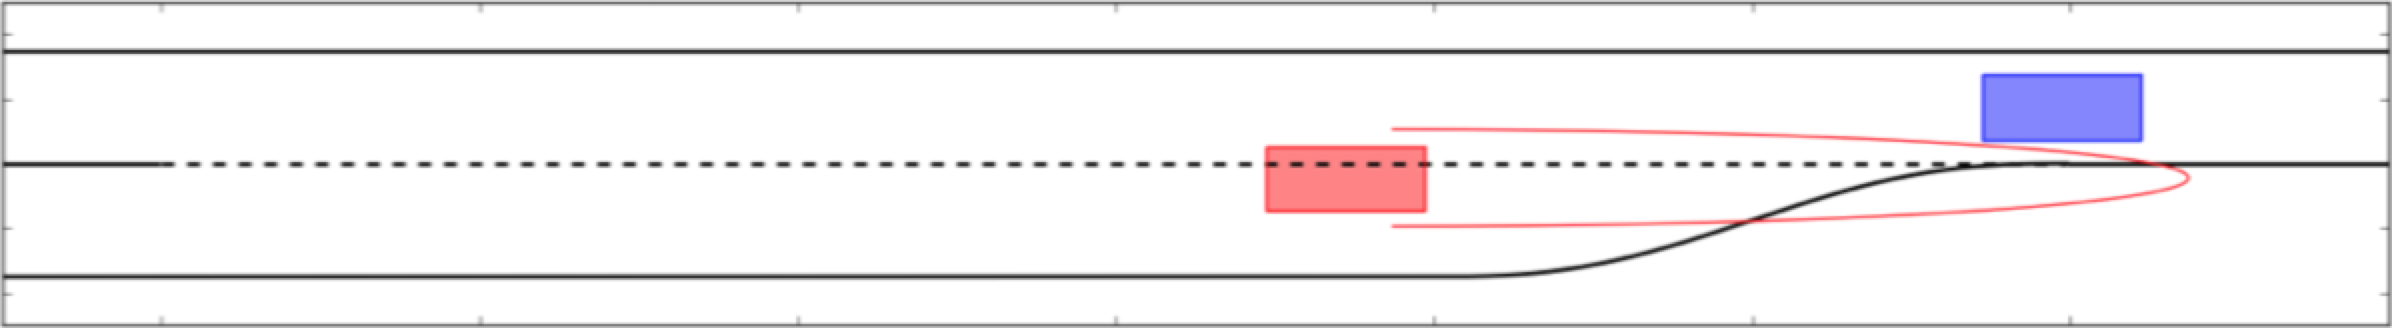
\includegraphics[width =  \textwidth]{Einhalten.png}
    }
    \subfigure[Sicherheitsabstand wird unterschritten (\( d_\mathrm{normal} = 0,85 \)).]{
        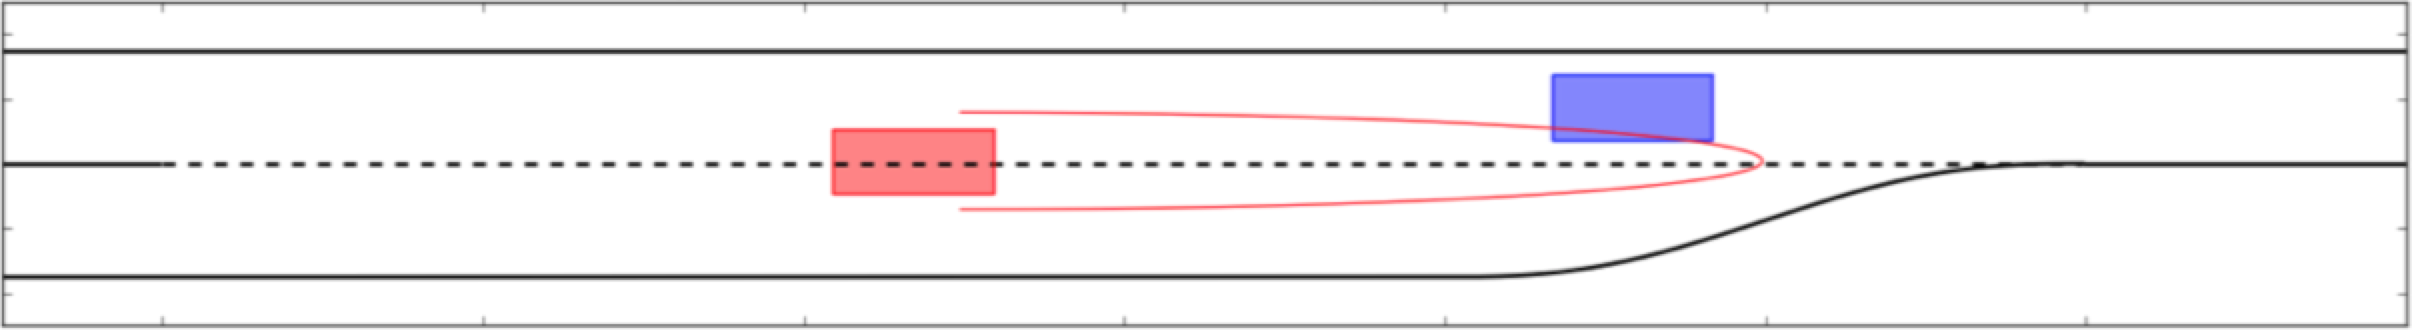
\includegraphics[width =  \textwidth]{Unterschreiten.png}
    }
    \caption[Normalisierter Sicherheitsabstand]{Normalisierter Sicherheitsabstand}
    \label{fig:NormSD}
\end{figure}



Um nun den Kostenterm \gls{symb:G_sd} zu berechnen wird ein normalisierter Sicherheitsabstand \gls{symb:d_normal} eingef\"uhrt.
Dieser hat den Wert Eins wenn sich ein anderes Fahrzeuge gerade am Rand des Sicherheitsbereiches befindet und den Wert Null wenn sich die beiden Fahrzeug gerade ber\"uhren.
Zwischen diesen beiden Werten wird linear interpoliert.
Durch den Kostenterm \gls{symb:G_sd} werden nun alle Abst\"ande die zu einem normalisierten Sicherheitsabstand f\"uhren der einen festgelegten Grenzwert unterschreitet mit entsprechenden Kosten bewertet.
Da ein Unterschreiten des Sicherheitsabstandes besonders sicherheitskritisch ist und von Menschen schnell als unangenehm empfunden wird, sollten die Kosten f\"ur das Unterschreiten des Sicherheitsabstandes vergleichsweise stark ansteigen.
Deshalb wird die Grenze zum diskomfortablen Bereich relativ nahe am Optimum gew\"ahlt.

Bei einem Fahrstreifenwechsel sollten die Fahrzeuge auf dem Zielfahrstreifen nicht zu einem sicherheitskritischem Bremsman\"over gezwungen werden \cite{Treiber2010}.
Im Idealfall findet der Fahrstreifenwechsel so statt, dass keine Verz\"ogerung notwendig ist.
Es wird deshalb der Kostenterm \gls{symb:G_lc} eingef\"uhrt. 
Damit werden Verz\"ogerungen bewertet zu denen die Fahrzeuge auf dem Zielfahrstreifen gezwungen w\"aren, wenn sie bis zum Ende des Fahrstreifenwechsels den geforderten Zeitabstand  \gls{symb:t_abs} einhalten wollen.
Dabei wird davon ausgegangen, dass die Verz\"ogerung bei \gls{symb:t_lc} eingeleitet wird und der Abstand bei \gls{symb:t_coop,end} genau eingehalten wird.
Am Ende des Fahrstreifenwechsels soll nun also ein Abstand \gls{symb:d_sd} eingehalten werden, der mit dem gew\"unschten Zeitabstand \gls{symb:t_abs} wie folgt berechnet wird:

\begin{equation}
	d_\mathrm{sd} =  T_\mathrm{abs}  v_\mathrm{t,lc}^{follow}.
\end{equation}

Der Wert \(v_\mathrm{t,lc}^{follow}\) beschreibt die Geschwindigkeit des Folgefahrzeuges auf dem Zielfahrstreifen zum Zeitpunkt \gls{symb:t_lc}.
Der Abstand \( d_\mathrm{t,end,coop}\) der beiden Fahrzeuge am Ende des Verz\"ogerungsvorgangs kann wie folgt berechnet werden:

\begin{equation}
	d_\mathrm{t,end,coop} = d_\mathrm{t,lc} + v_\mathrm{t,lc}^{change} \Delta t- \left( v_\mathrm{t,lc}^{follow} \Delta t+ 0,5 * b_\mathrm{nece} \Delta t^2 \right)
\end{equation}

Dabei ist \gls{symb:d_tlc} der Abstand der beiden Fahrzeuge zum Zeitpunkt \gls{symb:t_lc}, \(v_\mathrm{t,lc}^{change}\) die Geschwindigkeit des fahrstreifenwechselnden Fahrzeuges zum Zeitpunkt \gls{symb:t_lc} und \gls{symb:b_nece} die gesuchte notwendige Verz\"ogerung.
Der Wert \(\Delta t\)  ergibt sich zu \gls{symb:t_coop,end} - \gls{symb:t_lc}.
Durch Gleichsetzten von \gls{symb:d_sd} und \(d_\mathrm{t,end,coop}\) und anschlie{\ss}endem ausfl\"osen nach \(b_\mathrm{nece}\) ergibt sich die folgende Formel:

\begin{equation}
	b_\mathrm{nece} = \frac{d_\mathrm{t,lc} + \left( v_\mathrm{t,lc}^{change} - v_\mathrm{t,lc}^{follow} \right) \Delta t -    T_\mathrm{abs} v_\mathrm{t,lc}^{follow}}{T_\mathrm{abs}  \Delta t + 0,5 * \Delta t^2}
\end{equation}
Durch den Kostenterm \gls{symb:G_lc} werden nur negative Werte von \gls{symb:b_nece} mit Kosten bewertet.


Dadurch dass die Kosten der kooperativen Fahrzeuge nur bis \gls{symb:t_coop,end} ber\"ucksichtigt werden und die Kosten des Ego"=Fahrzeuges dar\"uber hinaus, wird das Ego"=Fahrzeug in der Optimierung bevorzugt.
Bei der gleichen Trajektorie des Ego"=Fahrzeuges und eines kooperativen Fahrzeuges verursacht die Trajeketorie des Ego"=Fahrzeuges bei gleichem Kostenfunktional h\"ohere Kosten, da sie auch nach \gls{symb:t_coop,end} Kosten verursacht.
Zur Minimierung der Kosten wird deshalb ein Trajektorieset angestrebt bei dem die Geschwindigkeit des Ego"=Fahrzeuges m\"oglichst nahe an dessen Optimalgeschwindigkeit ist.
Die Geschwindigkeitsabweichnung des kooperativen Fahrzeuges f\"allt weniger ins Gewicht.
Um dies zu vermeiden wird der Kostenterm \gls{symb:G_lcend} eingef\"uhrt.
Durch ihn wird der Zustand der kooperierenden Fahrzeuge zum Zeitpunkt \gls{symb:t_coop,end} bewertet.
Dadurch k\"onnen auch Kosten \"uber \gls{symb:t_coop,end} hinaus abgebildet werden.

Zur Berechnung des Kostenterms wird eine Beschleunigung \gls{symb:a_lcend} aus dem komfortablen Bereich gew\"ahlt.
Anschlie{\ss}end wird berechnet welche Zeit \(t_\mathrm{accel}\) ben\"otigt wird um vom Zustand des kooperativen Fahrzeuges zum Zeitpunkt \gls{symb:t_coop,end}  auf die gew\"unschte Optimalgeschwindigkeit zu beschleunigen.
Dabei wird von einer konstanten Beschleunigung mit \gls{symb:a_lcend} ausgegangen.
Es wird au{\ss}erdem die mittlere Geschwindigkeit \( \bar{v}_\mathrm{lc,end} \) f\"ur den Beschleunigungsvorgang bestimmt.
Der Kostenterm \gls{symb:G_lcend} ergibt sich nun aus der Berechnung der dynamischen Kosten bei einer konstanten Beschleunigung \(a_\mathrm{lc,end} \) und einer als konstant angenommenen Geschwindigkeit  \( \bar{v}_\mathrm{lc,end} \) \"uber einen Zeitraum von \gls{symb:t_coop,end} bis \gls{symb:t_coop,end} +  \( t_\mathrm{accel}\).
Ist  \gls{symb:t_coop,end} +  \(t_\mathrm{accel}\) gr\"o{\ss}er als der Planungshorizont werden die dynamischen Kosten von \gls{symb:t_coop,end} bis zum Ende des Planungshorizonts berechnet.


\subsection{Fahrstreifenbasierte Pr\"adiktion}
\label{sec:IDMpred}
Die Bewegunspr\"adiktion anderer Fahrzeuge ist eine entscheidende Herausforderung f\"ur automatisierte Fahrzeuge.
Hier wird pr\"adiziert, wie sich eine Verkehrssituation in n\"achster Zukunft entwickeln wird.
Dabei werden die zuk\"unftigen Positionen und Zust\"ande der einzelnen Fahrzeuge vorherbestimmt \cite{Hermes2009}.
Dies ist notwendig um potentielle Risiken m\"oglichst fr\"uh zu erkennen.
Beruhend darauf kann dann eine Trajektorieplanung stattfinden.

Grundsteine von Bewegungspr\"adiktionen sind Bewegungsmodelle.
Durch sie wird bestimmt, wie sich die Fahrzeuge im aktuellen Szenario verhalten werden.
Lef\`{e}vre et al. \cite{Lefevre2014} teilen die Bewegungsmodelle in drei Gruppen steigender Komplexit\"at auf:

\begin{enumerate}
\item \textit{Physik"=basierte Bewegungsmodelle}: Die Bewegung der Fahrzeuge h\"angt ausschlie{\ss}lich von Gesetzten der Physik ab
\item \textit{Man\"overbasierte Bewegungsmodelle}: Die Bewegung h\"angt zus\"atzlich von Man\"overn ab, die der Fahrer plant durchzuf\"uhren
\item \textit{Interaktionsber\"ucksichtigende Bewegungsmodelle}: Die Wechselbeziehung von Man\"overn verschiedener Fahrzeuge wird ber\"ucksichtigt.
\end{enumerate}

Zu den einfachsten Bewegungsmodellen geh\"oren die Bewegungsmodelle der konstanten Geschwindigkeit und der konstanten Beschleunigung.
Sie werden den Physik"=basierten Bewegungsmodellen zugeordnet.
Physik"=basierte Bewegungsmodelle sind die am meisten benutzten Bewegungsmodelle zur Trajektorienp\"ardiktion \cite{Lefevre2014}.
Allerdings sind sie auf sehr kurze Pr\"adiktionshorizonte limitiert, da sie nicht auf Ver\"anderungen der direkten Fahrzeugumgebung, wie einem langsam fahrenden Fahrzeug, reagieren k\"onnen.
Werden andere Aspekte wie Unsicherheiten bei der Sch\"atzung der aktuellen Fahrzeugzust\"ande und Interaktionen zwischen Fahrzeugen ber\"ucksichtigt nimmt die Komplexit\"at stark zu.

Wird jedoch angenommen, dass keines der Fahrzeuge w\"ahrend des Planungshorizonts seinen Fahrstreifen wechselt, vereinfacht sich die Situation erheblich.
Das Bewegungsmodell h\"angt nun ma{\ss}geblich von der eigenen Wunschgeschwindigkeit und dem vorausfahrenden Fahrzeug ab.
Damit kann auf g\"angige Einspur"=Fahrzeugfolgemodelle zur\"uckgegriffen werden.
Auch heutige Adaptive Cruise Control (ACC) Systeme beruhen auf Modellen dieser Art.
Der Schwerpunkt dieser Arbeit liegt nicht auf der Bewegungsp\"adiktion.
Deshalb soll die vereinfachende Annahme getroffen werden, dass alle anderen Fahrzeuge in der Umgebung des Ego"=Fahrzeuges ihren Fahrstreifen innerhalb des Planungshorizontes beibehalten.
Damit kann sowohl f\"ur die vom Ego"=Fahrzeug unabh\"angige Bewegunspr\"adiktion also auch f\"ur die Neupr\"adiktion nach dem Fahrstreifenwechsel ein Fahrzeugfolgemodel verwendet werden.
Die Pr\"adiktion findet f\"ur jeden Fahrstreifen einzeln statt.
Diese Annahme kann jedoch durch Verwendung eines anderen Pr\"adiktionsverfahren aufgelockert werden.
F\"ur das Einspur"=Fahrzeugfolgemodel wurde sich f\"ur das von Treiber et al. \cite{Treiber2000} vorgestellte \gls{idm} entschieden.
Dies wird im Folgenden vorgestellt.


\minisec{Intelligent Driver Model}
Das Intelligent Driver Model ist ein zeitkontinuierliches Einspur"=Fahrzeugmodell.
Es geh\"ort zu einem der bekanntesten und meist angewendeten Fahrzeugmodellen.
Es wird unter anderem in \cite{Schwarting2014} und \cite{Hubmann2018} verwendet um das Standartverhalten der Fahrzeuge abzubilden.
Laut Schwarting et al. \cite{Schwarting2014} ist damit eine realistische Simulation der Verkehrsszene innerhalb des Planungshorizonts m\"oglich.
Dies gilt nur unter der Annahme, dass keine Fahrstreifenwechsel stattfinden.
Das \gls{idm} weist einige Vorteile gegen\"uber anderen Einspur"=Fahrzeugfolgemodellen auf.
So werden realistische Beschleunigungen ermittelt, es werden keine Unf\"alle erzeugt und es ist auch bei nicht dichtem Verkehr anwendbar.
Die Fahrzeugdynamik wird, wie bei den meisten Fahrzeugfolgemodellen, durch eine Beschleunigungsfunktion beschrieben \cite{Treiber2000}.
Durch Integration der Beschleunigung kann dann die Geschwindigkeit und die Position des Fahrzeuges berechnet werden.
In Vergleich zu anderen Fahrzeugefolgemodellen werden viele Parameter ber\"ucksichtigt:

\begin{itemize}
\item \textit{Wunschgeschwindigkeit} \( v_{0} \): Die Geschwindigkeit, die das Fahrzeug ohne Verkehr fahren w\"urde
\item \textit{Minimalabstand} \(s_{0}\): Minimal gew\"unschter Abstand zum vorausfahrenden Fahrzeug
\item \textit{Gew\"unschte Zeitl\"ucke} \( T \): Gew\"unschter Zeitabstand zum vorausfahrenden Fahrzeug
\item \textit{Maximale Beschleunigung} \( a \): Maximale Beschleunigung des Fahrzeuges
\item \textit{Komfortable Verz\"ogerung} \( b \): Verz\"ogerung die beim Bremsen gerade noch als komfortabel angesehen wird. (Es wird ein positiver Wert eingesetzt)
\item \textit{Beschleunigungsexponent} \( \delta \): Beschreibt wie die Beschleunigung beim Ann\"ahern an die Zielgeschwindigkeit abklingt
\item \textit{Geschwindigkeitsunterschied} \( \Delta v_\alpha \): Aktueller Geschwindigkeitsunterschied zwischen den beiden Fahrzeugen
\item \textit{Abstand \( s_\alpha \)}: Aktueller Abstand zwischen den beiden Fahrzeugen, gemessen von der Sto{\ss}stange des Fahrzeuges bis zum Heck des vorausfahrenden Fahrzeuges.
\end{itemize}

Es ergibt sich folgende Formel:

\begin{equation}
   \dot{v}_\alpha = a \left( 1 - \left( \frac{v_\alpha}{v_0}^\delta \right) - \left( \frac{s^*(v_\alpha, \Delta v_\alpha)}{s_\alpha}\right)^2\right).
\end{equation}

Es wird sowohl die aktuelle Geschwindigkeit \( v_\alpha\) mit der Wunschgeschwindigkeit \( v_{0} \) verglichen als auch der aktuelle Abstand \( s_\alpha \) mit dem Wunschabstand \( s^*\).
Der Wunschabstand
\begin{equation}
   s^*(v_\alpha, \Delta v_\alpha) =  s_0 + max \left( 0, v_\alpha T + \frac{v_\alpha \Delta v_\alpha}{2 \sqrt{ab}}\right)\end{equation}
enth\"alt neben einem Gleichgewichtsanteil \(s_0 + v_\alpha T \) auch einen dynamischen Anteil gegeben durch \( (v_\alpha \Delta v_\alpha)/(2 \sqrt{ab}) \).

Die Beschleunigungsformel l\"asst sich in einen freie Fahrt Term

\begin{equation}
   \dot{v}_\alpha^{free} = a \left( 1 - \left( \frac{v_\alpha}{v_0} \right) ^\delta \right)
\end{equation}

und einen interaktiven Term 

\begin{equation}
   \dot{v}_\alpha^{int} = - a \left( \frac{s^*(v_\alpha, \Delta v_\alpha)}{s_\alpha} \right)^2
\end{equation}

einteilen.
Der Term \( \dot{v}_\alpha^{free} \) beschreibt das Verhalten des Fahrzeuges bei freier Fahrt.
Der Term \( \dot{v}_\alpha^{int} \) beschreibt das Verhalten des Fahrzeuges wenn es aufgrund des Verkehrs nicht mehr mit der Wunschgeschwindigkeit fahren kann.


\subsection{Pfadplanung}
\label{sec:Pfadplanung}
Ein Pfad f\"ur einen einzelnen Fahrstreifenwechsel kann in drei Teilabschnitte eingeteilt werden: dem Pfad des aktuellen Fahrstreifens, dem Pfad des Zielfahrstreifens und dem Fahrstreifenwechselpfad.
Die drei Teilabschnitte sind in Abbildung~\ref{fig:Pfad} dargestellt.
Soll eine Trajektorie mehr als einen Fahrstreifenwechsel beinhalten, kann der Pfad aus mehreren einzelnen Fahrstreifenwechseln zusammengesetzt werden.
Die Funktion \gls{symb:F_init} zur Beschreibung des Pfades des aktuellen Fahrstreifen und die Funktion \gls{symb:F_target} zur Beschreibung des Pfades des Zielfahrstreifen sollen als gegeben angenommen werden.
Der Verlauf dieser Pfade ist durch die Fahrbahnmakierungen weitestgehend vorgegeben und kann in einer Karte hinterlegt werden.
In den meisten F\"allen wird der Verlauf angen\"ahert durch einen Polygonzug beschrieben.
Um den Pfad f\"ur das komplette Fahrstreifenwechselman\"over vollst\"andig beschreiben zu k\"onnen m\"ussen noch die geometrischen Punkte \( P_\mathrm{lc}^\mathrm{start}\) und \( P_\mathrm{lc}^\mathrm{end}\) festgelegt werden.
Sie beschrieben an welchem Punkt der Fahrstreifenwechsel eingeleitet wird und an welchem Punkt der Fahrstreifenwechsel beendet ist.
Des Weiteren muss die geometrische Verbindung der Punkte festgelegt werden.

\begin{figure}[!htbp]
    \centering
    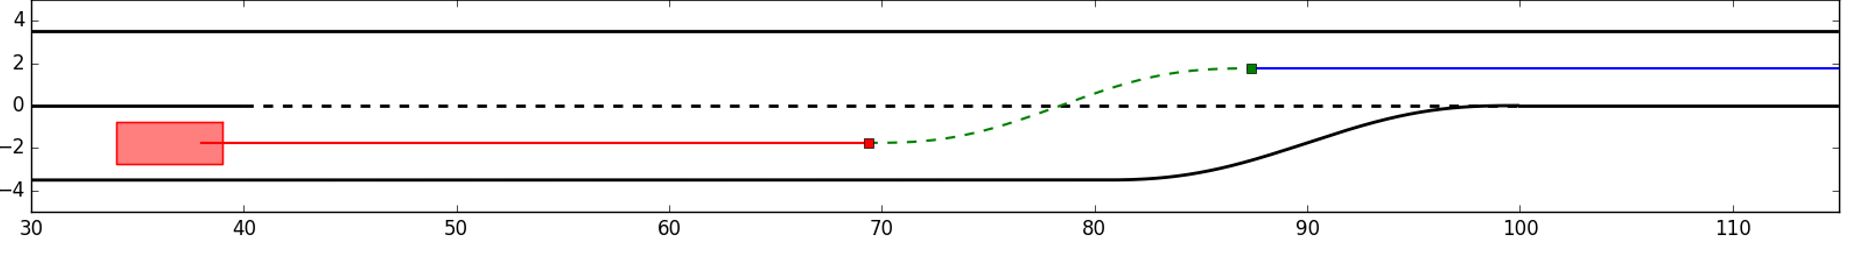
\includegraphics[width = 0.95 \textwidth ]{Pfad.png}
    \caption[Pfadplanung]{Pfad f\"ur einzelnen Fahrstreifenwechsel zusammengesetzt aus: Pfad des aktuellen Fahrstreifens (rot durchgezogen), Fahrstreifenwechselpfad (gr\"un gestrichelt), Pfad des Zielfahrstreifens (blau durchgezogen). Au{\ss}erdem dargestellt  \( P_\mathrm{lc}^\mathrm{start}\) (rot) und \( P_\mathrm{lc}^\mathrm{end}\) (blau)}
    \label{fig:Pfad}
\end{figure}


Wie in Kapitel~\ref{sec:FrenetBesch} erl\"autert, findet die Pfadplanung in Frenet"=Koordinaten statt.
Es ist au{\ss}erdem festgelegt, dass der Punkt \( P_\mathrm{lc}^\mathrm{start}\) auf dem Pfad des aktuellen Fahrstreifens liegt und das der Punkt \( P_\mathrm{lc}^\mathrm{end}\) auf dem Pfad des Zielfahrstreifens liegt.
Die Punkte sind demnach vollst\"andig beschrieben, wenn bekannt ist ab welcher Wegstrecke \gls{symb:s_cs} entlang der Referenzkurve der Fahrstreifenwechsel beginnt und ab welcher Westrecke \gls{symb:s_ce} der Fahrstreifenwechsel endet.
Die Funktion \gls{symb:F_lc}(s) zur Beschreibung des Gesamtpfades kann also wie folgt formuliert werden:

\begin{equation}
  F_\mathrm{lc}(s) = 
  \begin{cases} 
    F_\mathrm{init}                         & \quad , s \leq s_\mathrm{change}^\mathrm{start}\\ 
    F_\mathrm{change}                  & \quad , s_\mathrm{change}^\mathrm{start} < s \leq s_\mathrm{change}^\mathrm{end}\\ 
    F_\mathrm{target}                     & \quad , s > s_\mathrm{change}^\mathrm{end}.
  \end{cases} 
  \label{eqn:Kostenfunktion}
\end{equation}

Dabei ist \gls{symb:F_change} die Funktion des Fahrstreifenwechselpfades in Frenet"=Koordinaten.
Die noch zu ermittelnden Unbekannten sind der Start des Fahrstreifenwechsels \gls{symb:s_cs}, das Ende des Fahrstreifenwechsels \gls{symb:s_ce} und die Funktion \gls{symb:F_change}, die die beiden Punkte verbindet.
Die Pfadplanung soll aufgrund eines vorgegebenen Geschwindigkeitsprofiles generiert werden.

\minisec{Ermittlung des Fahrstreifenwechselsstartpunktes}
Um den Startpunkt des Fahrstreifenwechsels zu ermitteln ist es zun\"achst sinnvoll, noch einmal zu betrachten, aus welchen Gr\"unden Fahrstreifenwechsel durchgef\"uhrt werden.
Wie in Kapitel~\ref{sec:AuswahlBA} beschrieben, werden Fahrstreifenwechsel in notwendige und frei verf\"ugbare Fahrstreifenwechsel eingeteilt.
Fahrstreifenwechsel k\"onnen entweder notwendig sein, um einem vorgegebenen Pfad zu folgen oder weil der aktuelle Fahrstreifen endet.
Ein freiwilliger Fahrstreifenwechsel wird in der Regel durchgef\"uhrt um m\"oglichst mit der aktuellen Wunschgeschwindigkeit zu fahren.

Der einfachste Fall zur Bestimmung des Startpunktes des Fahrstreifenwechsels ergibt sich, wenn vorgegeben ist, dass sich am Ende des aktuellen Fahrstreifens nach dem Rei{\ss}verschlussverfahrens auf dem Zielfahrstreifen einzuordnen ist.
Der Bereich in dem der Fahrstreifenwechsel eingeleitet werden sollte ist somit stark eingeschr\"ankt.
Bei einer Beschleunigungsspur gilt das Rei{\ss}verschlussverfahren nicht.
Das gleiche gilt f\"ur Fahrstreifenwechsel die aufgrund der vorgegebenen Route durchgef\"uhrt werden m\"ussen.
Bei Fahrstreifenwechseln dieser Art ist deutlich schwerer festzulegen, wann ein Fahrstreifenwechsel eingeleitet werden soll.
Dies h\"angt stark von anderen Fahrzeugen ab.
Der Fahrstreifenwechsel kann ab einer Wegstrecke \gls{symb:s_cmin} eingeleitet werden und sollte sp\"atestes bis zu einer Wegstrecke  \gls{symb:s_cmax} eingeleitet werden, da danach der Fahrstreifenwechsel nicht mehr m\"oglich ist.
Es wird davon ausgegangen, dass auch diese Informationen in der Karte hinterlegt sind.
Ein fr\"uher Fahrstreifenwechsel f\"uhrt m\"oglicherweise dazu, dass die Geschwindigkeit des Zielfahrstriefens noch nicht erreicht werden konnte oder aber, dass den Fahrzeugen auf dem Zielfahrstreifen nicht gen\"ugend Zeit bleibt ihre Geschwindigkeit f\"ur eine Kooperation anzupassen.
Ist der Fahrstreifenwechsel erst sp\"at geplant und kann unerwarteter Weise doch nicht ausgef\"uhrt werden, ist das Fahrzeug wom\"oglich gezwungen kurz vor dem Ende des aktuellen Fahrstreifens anzuhalten.
Dies erschwert den gewollten Fahrstreifenwechsel noch mehr.

In vielen F\"allen wird zur Planung des Fahrstreifenwechsels zuerst eine m\"oglichst vielversprechende L\"ucke ausgew\"ahlt.
Anschlie{\ss}end wird das Geschwindigkeitsprofil des Fahrzeuges so gew\"ahlt, dass das Fahrzeug sich dieser L\"ucke ann\"ahert.
Ist die L\"ucke gro{\ss} genug kann der Fahrstreifenwechsel vollzogen werden.
Ist sie noch nicht gro{\ss} genug kann abgewartet werden, ob die Fahrzeuge auf dem Zielfahrstreifen ihre Geschwindigkeit anpassen um die L\"ucke zu vergr\"o{\ss}ern.
Die Auswahl der richtigen L\"ucke und die anschlie{\ss}ende Planung des Fahrstreifenwechsels sind keine trivialen Aufgaben.
Sie f\"ur jedes einzelne erzeugte Geschwindigkeitsprofil des Ego"=Fahrzeuges zu l\"osen ist mit einem hohen Rechenaufwand verbunden.
Es wurde deshalb entschieden \gls{symb:s_cs} als weiteren Parameter im Optimierungsproblem zu ber\"ucksichtigen.
Dazu wird bei der Pfadplanung eine zuf\"allige Wegstrecke \gls{symb:s_cs} zwischen den beiden Grenzwerten \gls{symb:s_cmin} und \gls{symb:s_cmax} ermittelt.
Durch die Vielzahl der ermittelten Trajektoriensets kann dadurch der optimale Zeitpunkt zur Einleitung des Fahrstreifenwechsels angen\"ahert werden.


Bei einem freiwilligen Fahrstreifenwechsel der durchgef\"uhrt wird um ein langsameres Fahrzeug zu \"uberholen, kann bei einem gegebenen Geschwindigkeitsprofil des Ego"=Fahrzeuges der Zeitpunkt des Fahrstreifenwechsels vom vorausfahrenden Fahrzeug abh\"angig gemacht werden.
Es kann festgelegt werden, dass der Fahrstreifenwechsel zu einem vorgeschriebenen Zeitpunkt \(t_\mathrm{cbc} \) bevor es zur Kollision mit dem vorausfahrenden Fahrzeug kommt, eingeleitet wird.
Hierzu kann die in der ISO 15623:2013 \gls{isoettc} definierte \gls{ettc} berechnet werden:

\begin{equation} 
	ETTC := \frac{- \Delta \dot{s} - \sqrt{\left( \Delta \dot{s} \right)^2 - 2 \Delta \ddot{s} \Delta \dot{s}}}{\Delta \ddot{s}}.
\end{equation}

Sobald die Bedingung \(ETTC \leq t_\mathrm{cbc}\) erf\"ullt ist wird der Fahrstreifenwechsel eingeleitet.
Zur Ermittlung von \gls{symb:s_cs} wird nun die Bewegungspr\"adiktion der anderen Fahrzeuge genutzt und berechnet, wann diese Bedingung eintrifft.

\minisec{Ermittlung des Fahrstreifenwechselsendpunktes}
Bei gegebenem Startpunkt des Fahrstreifenwechsels soll nun ein Endpunkt des Fahrstreifenwechsels ermittelt werden.
Die L\"ange des Fahrstreifenwechsels sollte von der Geschwindigkeit des Fahrzeuges abh\"angen.
Wird ein Fahrstreifenwechsel zu schnell ausgef\"uhrt, f\"uhrt dies zu hohen lateralen Beschleunigungen.
Werling \cite{Werling2011} generiert zur Ermittlung der Fahrstreifenwechseltrajektorie eine Trajektorienschar mit unterschiedlichen Endzust\"anden.
Aus der Trajektorienschar wird die Trajektorie ausgew\"ahlt, die die geringsten Kosten verursacht.
Ein \"ahnliches Vorgehen w\"are auch in dem in dieser Arbeit vorgestellten Ansatz m\"oglich.
Dazu k\"onnten Fahrstreifenwechselpfade mit einer nicht fest vorgschriebenen L\"ange ermittelt werden.
Dies w\"urde jedoch zu einem weiteren Optimierungsparameter f\"uhren.

Es wird deshalb eine konstante, geschwindigkeitsunabh\"angige Dauer \gls{symb:t_lcd} f\"ur den Fahrstreifenwechsel festgelegt.
Die Wegstrecke \"uber die der Fahrstreifenwechsel stattfindet nimmt damit linear mit der Geschwindigkeit zu.
In \cite{Sporrer1998} wurde eine Untersuchung mit etwa 100 Fahrversuchen gemacht.
Diese ergab, dass die Dauer eines Fahrstreifenwechsels sich unabh\"angig von der gew\"ahlten Geschwindigkeit in einem Zeitraum von 3,1 bis 6,5 Sekunden bewegt.
Die gilt nicht in einer Notsituation.
Die Fahrstreifenwechsel wurden in drei Kategorien eingeteilt:

\begin{itemize}
\item \textit{Normaler Fahrstreifenwechsel}: Im Vordergrund steht das reine Wechseln des Fahrfahrstreifens.
\item \textit{Schneller Fahrstreifenwechsel}: Es wird Wert auf die Verringerung der Wechselzeit gelegt. Angestrebt werden soll das z\"ugige Wechseln in eine L\"ucke des flie{\ss}enden Verkehrs.
\item \textit{Notausweichman\"over}: Es soll einem pl\"otzlich auftauchendem Hindernis ausgewichen werden.
\end{itemize}

Ein schneller Fahrstreifenwechsel dauert 3,1 bis 4,7 Sekunden. 
Die Wegstrecke entlang der Referenzkurve an der der Fahrstreifenwechsel endet kann dann in guter N\"aherung wie folgt berechnet werden:

\begin{equation}
	s_\mathrm{change}^\mathrm{end} = s_\mathrm{change}^\mathrm{start} + t_\mathrm{lcd} v_\mathrm{lc,start}
\end{equation}

Dabei ist \( v_\mathrm{lc,start} \) die Geschwindigkeit des Fahrzeuges zu Beginn des Fahrstreifenwechsels.

\minisec{Fahrstreifenwechselpfad}

Sind sowohl \gls{symb:s_cs} und \gls{symb:s_ce} gegeben soll nun eine geometrische Verbindung zwischen dem sich daraus ergebenden Start- und Endpunkt des Fahrstreifenwechsels ermittelt werden.
Die Verbindung der beiden Punkte stellt den Fahrstreifenwechselpfad dar.
Der Fahrstreifenwechselpfad muss von der Kinematik des Fahrzeuges ausf\"uhrbar sein und sollte zu einer m\"oglichst komfortablen Trajektorie f\"uhren.
Die einfachste Verbindung w\"are eine Gerade.
Es ist jedoch offensichtlich, dass ein Fahrzeug einer solchen Verbindung nicht folgen kann.
Eine kubisches Polynom sorgt f\"ur eine Verbindung, bei der die Richtung an den Randpunkten mit den Randwerten der Spurpfade \"ubereinstimmt.
Jedoch kann keine Kr\"ummungsstetigkeit des Pfades garantiert werden.
Ein Sprung in der Kr\"ummung des Pfades macht jedoch ein sprunghaftes Einlenken notwendig.
Dies f\"uhrt nicht nur zu einem unkomfortablen Fahrverhalten sondern ist auch nicht zu realisieren \cite{Gnatzig2015}.
Es werden deshalb Polynome h\"oheren Grades ben\"otigt.
McNaughton \cite{Mcnau2011} verwendet deshalb quintische Polynome zur Erzeugung eines Pfades bei h\"oheren Geschwindigkeiten.

Auch in dieser Arbeit sollen f\"ur den Fahrstreifenwechselpfad ein quintisches Polynom verwendet werden.
Dies deckt sich gut mit der in Kapitel~\ref{sec:Varationsrechnung} gemachten Feststellung, dass eine ruckoptimale Trajektorie durch eine quintische Funktion beschrieben wird.
Zwar findet mit der Trajektorie eine zeitliche Beschreibung der Fahrzeugbewegung statt, jedoch ist diese Beschreibung praktisch equivalent zu der r\"aumlichen Beschreibung eines Pfades, wenn davon ausgegangen wird, dass das Fahrzeug mit einer konstanten Geschwindigkeit f\"ahrt \cite{Mcnau2011}.



\subsection{Klassifizierung}
Bei der Klassifizierung geht es in erster Linie darum festzustellen, welche Fahrzeuge durch ein kooperatives Verhalten zur Minimierung des Kostenfunktionals beitragen k\"onnen.
Die Trajektorie des Ego"=Fahrzeuges ist dabei durch das zuf\"allig ermittelte Geschwindigkeitsprofil und den daf\"ur ermittelten Pfad gegeben.
Um festzustellen zu k\"onnen welche Fahrzeuge f\"ur eine Kooperation in Frage kommen, soll an dieser Stelle der Fahrstreifenwechsel noch einmal genauer betrachtet werden.

Im Allgemeinen haben die Fahrzeuge auf dem Zielfahrstreifen ein Vorfahrtsrecht.
Ein Fahrzeug, dass den Fahrstreifen wechseln m\"ochte hat nun daf\"ur zu sorgen, dass es durch den Fahrstreifenwechsel nicht zu einer Gef\"ahrdung anderer Verkehrsteilnehmer kommt.
Dies bedeutet zum Einen, dass es daf\"ur verantwortlich ist w\"ahrend des Fahrstreifenwechsels den Sicherheitsabstand zum vorausfahrenden Fahrzeug auf dem aktuellen Fahrstreifen und auf dem Zielfahrstreifen einzuhalten.
Auf der anderen Seite muss es auch daf\"ur sorgen, dass es dem Folgefahrzeug auf dem Zielfahrstreifen m\"oglich ist den notwendigen Sicherheitsabstand einzuhalten.
Laut Treiber \cite{Treiber2010} darf als Konsequenz einer Entscheidung (also auch eines Fahrstreifenwechsels) keines der beteiligten Fahrzeuge gezwungen sein ein sicherheitskritisches Bremsman\"over durchzuf\"uhren.
Dies bedeutet, dass es dem Folgefahrzeug m\"oglich sein muss den Sicherheitsabstand einzuhalten ohne dabei eine Grenzverz\"ogerung \gls{symb:b_krit} zu \"uberschreiten.
Treiber schreibt, dass dieser Grenzwert in der Gr\"o{\ss}enordnung der komfortablen Bremsverz\"ogerung des \gls{idm} liegt (\( 2 m/s^2 \) ).
Sind die Abst\"ande zu den Fahrzeugen auf dem Zielfahrstreifen gro{\ss} genug, kann davon ausgegangen werden, dass das Ego"=Fahrzeug auch ohne kooperatives Verhalten anderer Fahrzeuge den Fahrstreifenwechsel sicher durchf\"uhren kann.

Die Fahrzeuge in der Umgebung des Ego"=Fahrzeuges werden in drei Gruppen eingeteilt:
\begin{itemize}
\item \textit{Beteiligte Fahrzeuge}: Fahrzeuge die durch ein kooperatives Verhalten zur Minimierung der Gesamtkosten beitragen k\"onnen.
\item \textit{Unbeteiligte Fahrzeuge}: Die Trajektorie der Fahrzeuge ist unabh\"angig vom Fahrstreifenwechsel des Ego"=Fahrzeuges.
\item \textit{Beeinflusste Fahrzeuge}: Die Fahrzeuge k\"onnen nicht direkt zur Minimierung der Kosten beitragen, m\"ussen aber m\"oglicherweise auf Grund des Fahrstreifenwechsels ihr Geschwindigkeitsprofil anpassen.
\end{itemize}

\begin{figure}[!htbp]
    \centering
    \subfigure[]{
        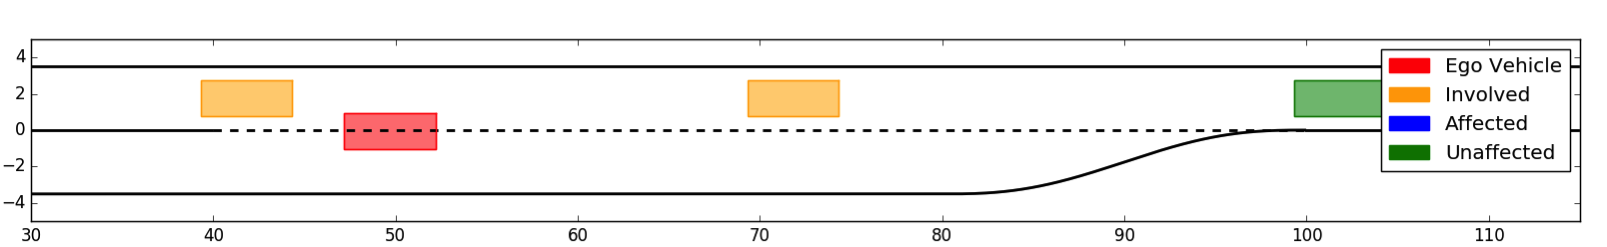
\includegraphics[width =  \textwidth]{Klassifizierung1.png}
    }
    \subfigure[]{
        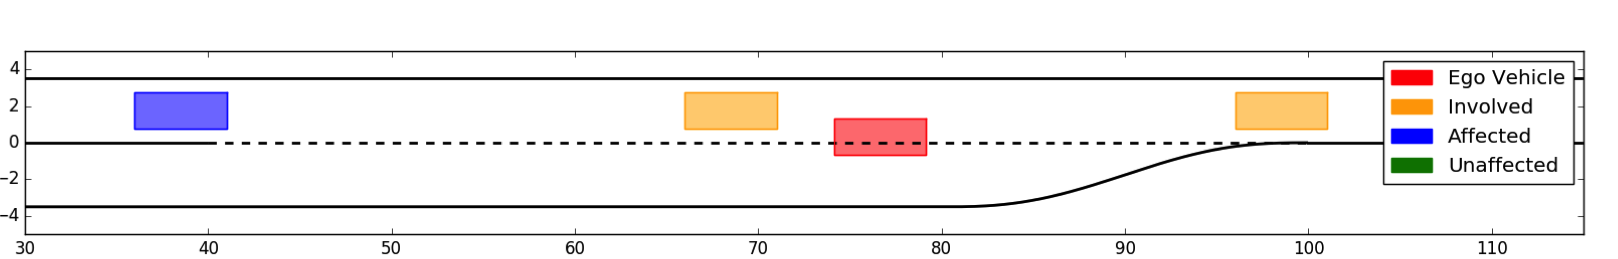
\includegraphics[width =  \textwidth]{Klassifizierung2.png}
    }
    \caption[Klassifizierung]{Klassifizierung der Fahrzeuge in der Umgebung der Ego"=Fahrzeuges (rot): beteiligte Fahrzeuge (gelb), unbeteiligte Fahrzeuge (gr\"un) und beeinflusste Fahrzeuge (blau)}
    \label{fig:Klassifizierung}
\end{figure}


Als beteiligte Fahrzeuge kommen das vorausfahrende und folgende Fahrzeug auf dem Zielfahrstreifen in Frage.
Es gilt nun zu pr\"ufen, ob die Abst\"ande zu diesen beiden Fahrzeugen auch ohne kooperatives Verhalten gro{\ss} genug sind um einen sicheren Fahrstreifenwechsel ausf\"uhren zu k\"onnen.
Daf\"ur wird nun die vom Ego"=Fahrzeug unabh\"angige Bewegungspr\"adiktion zum Zeitpunkt \gls{symb:t_lc} und die Trajektorie des Ego"=Fahrzeuges zum Zeitpunkt \gls{symb:t_lc} betrachtet.
Der Zeitpunkt \gls{symb:t_lc} wurde in Kapitel~\ref{sec:LCKostfunc} eingef\"uhrt und gibt den Zeitpunkt an, an dem das Ego"=Fahrzeug die Fahrbahnmakeriung \"uberquert.
Anhand der Bewegungspr\"adiktion und dem Zustand des Ego"=Fahrzeuges kann ermittelt werden, welches Fahrzeug sich zum Zeitpunkt \gls{symb:t_lc} vor und hinter dem Ego"=Fahrzeug auf dem Zielfahrstreifen befindet.
Ist der Abstand zum vorderen Fahrzeug bereits gr\"o{\ss}er als der geforderte Sicherheitsabstand kann davon ausgegangen werden, dass dieses kein kooperatives Verhalten zeigen wird.
Es wird als unbeteiligt eingestuft.
Ist er kleiner, so wird es als beteiligtes Fahrzeug klassifiziert.
Beim hinteren Fahrzeug muss als erstes gepr\"uft werden ob der Sicherheitsabstand zum Zeitpunkt \gls{symb:t_lc} gro{\ss} genug ist.
Ist dies der Fall muss ebenfalls gepr\"uft werden, ob es dem Fahrzeug m\"oglich ist durch eine Verz\"ogerung die geringer als \gls{symb:b_krit} ist den Sicherheitsabstand einzuhalten.
Dies muss nur gepr\"uft werden, falls die Geschwindigkeit des hinteren Fahrzeuges h\"oher ist als die des Ego"=Fahrzeuges.
In diesem Fall kann der mindestens notwendige Abstand \( d_\mathrm{nece} \) wie folgt berechnet werden:

\begin{equation}
	d_\mathrm{nece} =   T_\mathrm{abs} v_\mathrm{t,lc}^{follow} + \frac{\Delta v^2}{b_\mathrm{krit}} 
\end{equation}

Dabei ist \gls{symb:t_abs} der geforderte Zeitabstand,  \( v_\mathrm{t,lc}^{follow} \)  die Geschwindigkeit des hinteren Fahrzeuges zum Zeitpunkt \gls{symb:t_lc} und \( \Delta v \) der Geschwindigkeitsunterschied der beiden Fahrzeuge zum Zeitpunkt \gls{symb:t_lc}.
Ist der Abstand zum hinteren Fahrzeug gro{\ss} genug um diese Bedingungen zu erf\"ullen, wird davon ausgegangen, dass der Fahrstreifenwechsel ohne Kooperation stattfindet.
Das Fahrzeug wird als beeinflusst klassifiziert.
Andernfalls wird es als beteiligt eingestuft.

Die restlichen Fahrzeuge werden nun entweder als unbeteiligt oder beeinflusst eigestuft.
Fahrzeuge die sich weder auf dem aktuellen Fahrstreifen noch auf dem Zielfahrstreifen befinden werden als unbeteiligt klassifiziert.
Ebenso Fahrzeuge die sich zum Zeitpunkt \gls{symb:t_lc} vor dem Ego"=Fahrzeug befinden.
Die restlichen Fahrzeuge werden als beeinflusst eingestuft.
Die Klassifizierung der Fahrzeuge ist beispielshaft in Abbildung~\ref{fig:Klassifizierung} dargestellt.

Die Klassifzierung hat Auswirkungen darauf, wie die Fahrzeuge in den n\"achsten Schritten behandelt werden.
F\"ur beteiligte Fahrzeug wird in der inneren Optimierung ab \gls{symb:t_coop,start} bis \gls{symb:t_coop,end} eine kooperative Trajektorie ermittelt. 
Die restliche Trajektorie bis zum Ende des Planungshorizonts wird mittels dem in Kapitel~\ref{sec:IDMpred} vorgestellten \gls{idm} bestimmt.
Die unbeteiligten Fahrzeuge k\"onnen ihre urspr\"unglich ermittelte Trajektorie beibehalten.
Bei den beeinflussten Fahrzeugen wird davon ausgegangen, dass diese ab \gls{symb:t_coop,start} ihr Trajektorie anpassen m\"ussen.
F\"ur sie wird ab diesem Zeitpunkt bis zum Ende des Planungshorizonts eine neue Trajektorie anhand des \gls{idm}s bestimmt.


\subsection{Innere Optimierung}
F\"ur die als beteiligt klassifizierten Fahrzeuge soll nun die bestm\"ogliche kooperative Trajektorie gefunden werden.
Daf\"ur werden die Trajektorien im Zeitraum von \gls{symb:t_coop,start} bis \gls{symb:t_coop,end} neu bestimmt.
Werden sowohl das vordere als auch das hintere Fahrzeug auf dem Zielfahrstreifen als beteiligt klassifiziert, wird die Trajektorie zuerst f\"ur das vordere Fahrzeug ermittelt.
Anschlie{\ss}end wird auf Basis dessen die Trajektorie des folgenden Fahrzeuges ermittelt.
F\"ur jedes der Fahrzeuge wird nun ein inneres Optimierungsproblem gel\"ost.
Dabei soll die Summe aus den Kosten des beteiligten Fahrzeuges und den interaktiven Kosten des Ego"=Fahrzeuges minimiert werden.
Es ergibt sich das folgende Kostenfunktional

\begin{equation}
\label{Kostfunkin}
	G_\mathrm{lc,io} = G_\mathrm{bet,dyn} + \sum_j G_\mathrm{bet,j} + \sum_j G_\mathrm{ego,j}.
\end{equation}

\(G_\mathrm{bet,dyn}\) sind die dynamischen Kosten des beteiligten Fahrzeuges. \(G_\mathrm{bet,j}\) und \(G_\mathrm{ego,j}\) sind die Kosten des beteiligten Fahrzeuges und des Ego"=Fahrzeuges die Interaktion mit anderen Fahrzeugen entstehen.

Das Optimierungsproblem muss f\"ur den Zeitraum von \gls{symb:t_coop,start} bis \gls{symb:t_coop,end} gel\"ost werden.
Zur L\"osung dieses inneren Optimierungsproblems wurde sich erneut f\"ur ein samplingbasiertes L\"osungsverfahren entschieden.
Mit dem in Kapitel~\ref{sec:SmapPVD} vorgestellten Verfahren des Basisalgorithmus wird eine Vielzahl von Geschwindigkeitsprofilen f\"ur das beteiligte Fahrzeug erstellt.
Dabei ist der Ausgangszustand der Zustand des beteiligten Fahrzeuges zum Zeitpunkt \gls{symb:t_coop,start}.
Da der Pfad gegeben ist ergibt sich eine Vielzahl von Trajektorien.
F\"ur jede erzeugte Trajektorie werden nun die Kosten anhand des Kostenfunktionals~\ref{Kostfunkin} berechnet.
Anschlie{\ss}end wird die Trajektorie ausgew\"ahlt, die die geringsten Kosten verursacht.


\subsection{Zweifacher Fahrstreifenwechsel}
In Kapitel~\ref{sec:FrenetBesch} wird darauf eingegangen, dass ein doppelter Fahrstreifenwechsel, bei dem zwei Fahrstreifenwechsel in die gleiche Richtung ausgef\"uhrt werden, ausgeschlossen wird.
Ein Fahrstreifenwechsel auf den Zielfahrstreifen und wieder zur\"uck auf den Ausgangsfahrstreifen soll hingegen erm\"oglicht werden.
Das Wechseln auf den Zielfahrstreifen und Zur\"uckwechseln auf den Ausgangsfahrstreifen soll hier als zweifacher Fahrstreifenwechsel bezeichnet werden.
Es soll nun noch einmal genauer erl\"autert werden, warum eine Trajektorienplanung einen zweifachen Fahrstreifenwechsel erm\"oglichen sollte.
Anschlie{\ss}end wird beschrieben, wie dies in dem beschrieben Ansatz zur kooperativen Trajektorienplanung eines Fahrstreifenwechsels umgesetzt werden kann.

\begin{figure}[!htbp]
    \centering
    \subfigure[Trajektorienplanung in der die Umfahrung eines Hindernisses in zwei zeitlich versetzten Planungsschritten stattfinden muss]{
        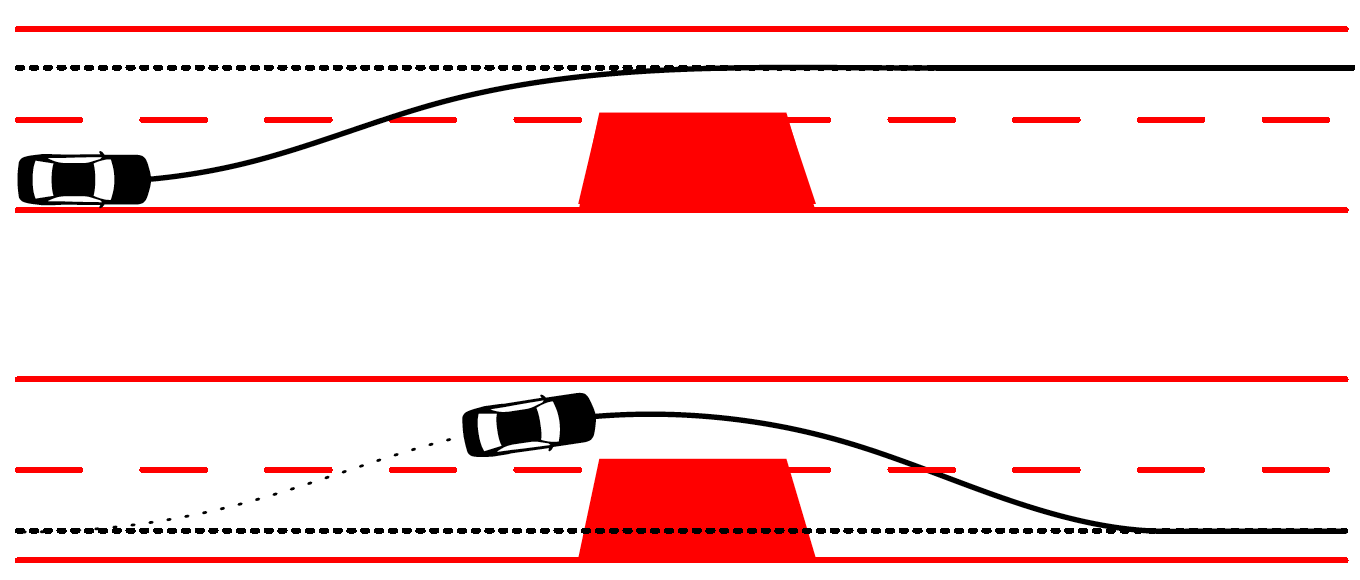
\includegraphics[width =  0.45 \textwidth]{ZweiPlanung.png}
        \label{fig:einfacherSpurw}
    }
    \hfill
    \subfigure[Trajektorienplanung in der die Umfahrung eines Hindernisses in einem Planungsschritt durchgef\"uhrt werden kann]{
        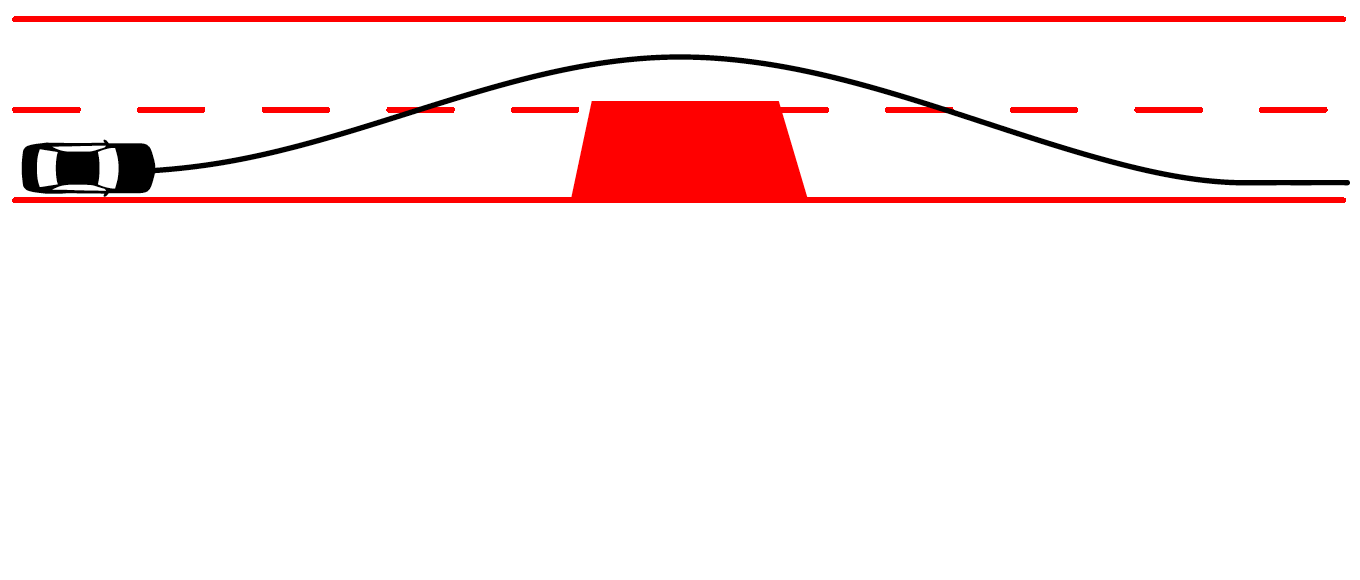
\includegraphics[width =  0.45 \textwidth]{EinPlanung.png}
        \label{fig:zweifacherSpurw}
    }
    \caption[Zweifacher Fahrstreifenwechsel]{Vergleich verschiedener Trajektorieplanungsans\"atze bei der Umfahrung eines Hindernisses \cite{Ziegler2017}}
    \label{fig:zweiSpurwech}
\end{figure}

In dem von Werling \cite{Werling2011} vorgestellten Ansatz zur Trajektorienplanung wird eine Trajektorie erzeugt, die durch ein quinitsches Polynom beschrieben wird.
Dadurch k\"onnen ruckoptimale Trajektorien generiert werden.
Ein solches Verfahren erlaubt die Planung eines einfachen Fahrstreifenwechsel in einem Planungsschritt.
Ziegler \cite{Ziegler2017} beschreibt die Suboptimalit\"at dieses Ansatzes.
Befindet sich ein Hindernis auf der Strecke wird zuerst eine Trajektorie erzeugt die dem Hindernis ausweicht (Abbildung~\ref{fig:einfacherSpurw} oben).
Erst in einem sp\"ateren Planungsschritt wird dann eine Trajektorie geplant, die wieder zur\"uck auf den Ausgangsfahrstreifen f\"uhrt (Abbildung~\ref{fig:einfacherSpurw} unten).
Eine Trajektorienplanung wie in Abbildung~\ref{fig:zweifacherSpurw} dargestellt, bei der in einem Planungsschritt sowohl das Ausweichen auf einen anderen Fahrstreifen als auch das Zur\"uckfahren auf den Ausgangsfahrstreifen geplant wird, ist nicht m\"oglich.

F\"ur das reine Umfahren eines Hindernisses ist ein Planungsansatz wie in Abbildung~\ref{fig:einfacherSpurw} dargestellt ausreichend.
Dieser Ansatz ger\"at jedoch an seine Grenzen, wenn ein \"ahnliches Man\"over bei entgegenkommenden Verkehr geplant werden soll.
Zu dem Zeitpunkt an dem der Fahrstreifenwechsel auf die Gegenspur eingeleitet wird, ist es der Trajektorienplanung noch nicht m\"oglich den Fahrstreifenwechsel zur\"uck auf den Ausgangsfahrstreifen zu planen.
Die Planung kann also vor Einleitung des Man\"overs nicht sicherstellten, dass der R\"uckwechsel ausgef\"uhrt werden kann bevor es zu einer Kollision mit dem entgegenkommendem Verkehr kommt.

Dies zeigt, dass ein Planungsverhalten wie in Abbildung~\ref{fig:zweifacherSpurw} gezeigt m\"oglich sein sollte.
In dem in Kapitel~\ref{sec:Pfadplanung} vorgestellten Teilschritt der Pfadplanung wird der Pfad f\"ur einen einfachen Fahrstreifenwechsel zu einem gegeben Geschwindigkeitsprofil erzeugt.
Erst anschlie{\ss}end wird in der inneren Optimierung und mit der Neupr\"adiktion vorherbestimmt wie die Fahrzeuge in der Umgebung des Ego"=Fahrzeuges auf diesen Fahrstreifenwechsel reagieren werden.
Die Reaktion der Fahrzeuge ist also im ersten Pfadplanungsschritt noch nicht bekannt.
Es k\"onnen deshalb in einem Pfadplanungsschritt nicht mehrere Fahrstreifenwechsel geplant werden, da der erste geplante Fahrstreifenwechsel das Verhalten der anderen Fahrzeuge beeinflusst.

F\"ur den vorliegenden Ansatz wird vorgeschlagen zun\"achst nur ein einzelnen Fahrstreifenwechsel zu planen und die Reaktion der anderen Fahrzeug auf diesen Fahrstreifenwechsel pr\"adiziert.
Ausgehend von dieser L\"osung werden dann die Schritte von der Pfadplanung bis zur Neupr\"adiktion wiederholt.
Ausgangspunkt f\"ur diesen zweiten Iterationsschritt sind die Zust\"ande der Fahrzeuge zum Zeitpunkt \gls{symb:t_coop,end}. 
Somit ist sichergestellt, dass die L\"osung der inneren Optimierung aus dem vorhergehenden Iterationsschritt erhalten bleibt.
Das Ergebnis ist ein Trajektorienset mit einer Egotrajektorie, die zwei Fahrstreifenwechsel enth\"alt.
Damit wird ein Planungsverhalten wie in Abbildung~\ref{fig:zweifacherSpurw} gezeigt erm\"oglicht.

F\"ur einen Fahrstreifenwechsel bei entgegenkommenden Verkehr ist darauf zu achten, dass hier nicht mehr der in Kapitel~\ref{sec:LCKostfunc} vorgestellte Zeitabstand \gls{symb:t_abs} verwendet werden kann.
Der Abstand zum entgegenkommenden Fahrzeug kann nicht mehr allein von der Geschwindigkeit des eigenen Fahrzeuges abh\"angig gemacht werden.
Hier sollte auf eine andere Vorgehensweise zur\"uckgegriffen werden.
Eine M\"oglichkeit bietet die Nutzung der von Naumann und Stiller \cite{Naumann2017towards} vorgestellten TZC (time of zone clearance).

\section{Fortlaufende Neuplanung}
\label{sec:Neuplanung}

Laut Hubmann et al. \cite{Hubmann2018} verursachen Unsicherheiten in der Pr\"adiktion der Trajektorie anderer Verkehrsteilnehmer eine hohe Komplexit\"at in der Trajektorieplanung.
Die Unsicherheiten ergeben sich aus:

\begin{itemize}
\item der unbekannten Route anderer Verkehrsteilnehmer,
\item den unbekannten longitudinalen Bewegungen anderer Fahrzeuge, 
\item potenziellen Interaktionen zwischen anderen Verkehrsteilnehmern und auch mit dem Ego"=Fahrzeug
\item und Ungenauigkeiten bei der Messung.
\end{itemize}

Die Ungenauigkeit in der Pr\"adiktion der Zust\"ande anderer Verkehrsteilnehmer nimmt zu, je weiter diese zeitlich vom aktuellen Zeitpunkt entfernt sind.
Je gr\"o{\ss}er die Ungenauigkeiten sind, desto schwieriger wird es f\"ur das automatisierte Fahrzeug eine sichere Trajektorie zu ermitteln.
Zus\"atzlich findet die Planung in der Regel in einem zeitlich begrenzten Horizont statt und auch die Sensoren des Fahrzeuges k\"onnen nur einen bestimmten Bereich abdecken.
Somit gelangen immer neue Bereiche der Umgebung in den Erfassungsbereich der Sensoren und es m\"ussen immer wieder neue Objekte in der Planung ber\"ucksichtigt werden.

Es ist offensichtlich, dass eine einmalige Planung, deren Trajektorie dann komplett ausgef\"uhrt wird, nicht umgesetzt werden kann.
Anstatt dessen wird bei automatisierten Fahrzeugen auf ein Vorgehen zur\"uckgegriffen, dass auch bei menschlichen Fahrern angewandt wird: die kontinuierliche Neuplanung.
Dabei wird die Planung in regelm\"a{\ss}igen Abst\"anden wiederholt.
Somit kann immer wieder auf die neue Erfassung der Umgebung reagiert werden.
Den Anfang der neu geplanten Trajektorie bildet dabei ein Teil der Trajektorie aus dem vorherigen Planungsschritt.
Damit kann eine Stetigkeit der letztendlich gefahrenen Trajektorie erreicht werden.
Das Vorgehen bei der fortlaufenden Neuplanung eines automatisierten Fahrzeuges wird von Ziegler \cite{Ziegler2017} beschrieben und ist in Abbildung~\ref{fig:Neuplanung} dargestellt.
In schwarz dargestellt ist die Trajektorie, die zum Zeitpunkt \gls{symb:t_jetzt} verf\"ugbar wurde.
Zu diesem Zeitpunkt wurde auch das rot schraffiert eingezeichnete Hindernis wahrgenommen.
Das Planungsmodul ben\"otigt maximal eine Zeit \gls{symb:t_verarb} zu Generierung der neuen Trajektorie.
Das bedeutet, dass das Fahrzeug von \gls{symb:t_jetzt} bis \gls{symb:t_jetzt} + \gls{symb:t_verarb} der schwarz eingezeichneten Trajektorie folgen muss (rot dargestellt).
Als Anfangswert zur Generierung der neuen Trajektorie wird nun der letzte Teil der alten Trajektorie aus dem Zeitbereich von \gls{symb:t_jetzt} bis \gls{symb:t_jetzt} + \gls{symb:t_verarb} genommen (blau dargestellt).
Ab \gls{symb:t_jetzt} + \gls{symb:t_verarb} wird nun die neue Trajektorie ausgef\"uhrt, die auf das erfasste Objekt reagiert und ihm ausweicht (gr\"un dargestellt).

\begin{figure}[!htbp]
    \centering
    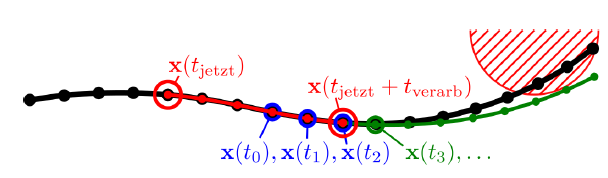
\includegraphics[width = 0.95 \textwidth]{Neuplanung.png}
    \caption[Neuplanung]{Darstellung der fortlaufenden Neuplanung \cite{Ziegler2017}}
    \label{fig:Neuplanung}
\end{figure}


Gerade in Situationen in denen es zur Interaktion mit anderen Verkehrsteilnehmern kommt ist es schwer vorherzusagen wie sich diese verhalten werden.
Eine fortlaufende Neuplanung ist somit unabdingbar.
In dem vorgestellten Ansatz wird dies umgesetzt, indem bei jedem Planungsschritt zwischen \gls{symb:t_jetzt} und \gls{symb:t_jetzt} + \gls{symb:t_verarb} der Pfad und das Geschwindigkeitsprofil der  Trajektorie aus dem vorausgegangenen Planungsschritt \"ubernommen wird.
Ab \gls{symb:t_jetzt} + \gls{symb:t_verarb} werden dann durch die zuf\"allige Generierung von R\"ucken randomisierte Geschwindigkeitsprofile erzeugt.
Alle diese Geschwindigkeitsprofile haben dadurch anf\"anglich den gleichen Verlauf.
F\"ur diese Geschwindigkeitsprofile wird dann jeweils ein Fahrstreifenwechselpfad generiert, wobei bis zum Zeitpunkt \gls{symb:t_jetzt} + \gls{symb:t_verarb} der bisherige Pfad \"ubernommen wird.

Die Trajektorien der anderen Fahrzeuge sind dem Planungsmodul unbekannt.
Im Gegensatz zum Ego"=Fahrzeug kann nicht davon ausgegangen werden, dass die anderen Fahrzeuge sich entsprechend des Ergebnisses des vorherigen Planungsschrittes verhalten werden.
Bei der Generierung der Geschwindigkeitsprofile der anderen Fahrzeuge wird als Ausgangspunkt deshalb nur der Zustand genommen der bei \gls{symb:t_jetzt} wahrgenommen wurde.
Die Geschwindigkeitsprofile werden f\"ur den gesamten Planungszeitraum neu generiert.

% !TeX root = ../thesis.tex

\chapter{Evaluation}
\label{sec:evaluation}
In diesem Kapitel findet die Evaluation des in Kapitel~\ref{sec:concepts} vorgestellten Ansatzes statt.
Zun\"achst werden die Szenarien vorgestellt, anhand denen der Ansatz evaluiert wird.
Anschlie{\ss}end wird auf die Implementierung des Ansatzes eingegangen.
Schlussendlich werden die Simulationsergebnisse vorgestellt und diskutiert. 
Dabei werden zun\"achst die Ergebnisse eines einzelnen Planungsschrittes untersucht.
Anschlie{\ss}end wird das verhalten des Ego"=Fahrzeuges bei einer fortlaufenden Neuplanung der Trajektorie betrachtet.


\section{Auswahl der Simulationsszenarien}
Der in Kapitel~\ref{sec:concepts} vorgestellte Ansatz soll simulativ getestet werden.
Da es im Rahmen dieser Arbeit zeitlich nicht m\"oglich ist alle Fahrstreifenwechselszenarien abzudecken, wird sich auf einige beispielhafte Szenarien beschr\"ankt.
Diese Szenarien soll die wichtigsten Aspekte des Ansatzes abdecken.

Ein Fahrstreifenwechselszenario bei dem sich am Ende des aktuellen Fahrstreifen nach dem Rei{\ss}verschlussverfahren auf dem neuen Fahrstreifen eingeordnet werden muss ist das einfachste Szenario.
Der Zeitpunkt an dem der Fahrstreifenwechsel eingeleitet werden sollte ist weitestgehend vorgegeben.
Es ist au{\ss}erdem in der Regel klar welche L\"ucke f\"ur den Fahrstreifenwechsel gew\"ahlt wird und es ist klar geregelt wie sich die Fahrzeuge zu verhalten haben.
Eine solche Verkehrssituation kann h\"aufig auch ohne einen kooperativen Ansatz gel\"ost werden. 
Ein freiwilliger Fahrstreifenwechsel, bei dem ein langsameres Fahrzeug \"uberholt werden soll stellt bereits eine schwierigere Aufgabe dar. 
Es muss zuerst eine geeignete L\"ucke ausgew\"ahlt werden.
Anschlie{\ss}end muss f\"ur diese L\"ucke ein Fahrstreifenwechsel geplant und ausgef\"uhrt werden.
Allerdings ist ein automatisiertes Fahrzeug in der Regel nicht auf den Fahrstreifenwechsel angewiesen.
Der Fahrstreifenwechsel kann so lange herausgez\"ogert werden bis sich eine L\"ucke ergibt, die gro{\ss} genug ist um einen Fahrstreifenwechsel durchzuf\"uhren, bei dem kein kooperatives Verhalten verlangt ist.
Dadurch muss das Fahrzeug zwar f\"ur eine gewisse Zeit von seiner Wunschgeschwindigkeit abweichen, es kommt aber in der Regel nicht zum Stillstand und stellt damit auch kein Sicherheitsrisiko dar.

Aus diesem Grund werden bei der Evaluierung ausschlie{\ss}lich Szenarien betrachtet, in denen ein notwendiger Fahrstreifenwechsel ausgef\"uhrt wird.
Bei einem solchen Szenario ist in der Regel vorgegeben ab wann der Fahrstreifenwechsel ausgef\"uhrt werden kann und bis wann er sp\"atestens vollzogen sein muss.
Um ein Stehenbleiben auf dem aktuellen Fahrstreifen zu vermeiden muss bei dichtem Verkehr deshalb in der Regel ein Fahrstreifenwechsel ausgef\"uhrt werden, der ein kooperatives Fahrverhalten verlangt.
Eine solches Szenario ergibt sich in der Haid"=und"=Neu"=Stra{\ss}e in Karlsruhe, Deutschland, die in der simulativen Evaluierung genutzt wurde.
Fahrzeuge die Links abbiegen wollen und auf dem rechten Fahrstreifen fahren, m\"ussen den Fahrstriefenwechsel vollzogen haben, bevor sich die beiden Fahrstreifen trennen (siehe Abbildung~\ref{fig:Szene}).

\begin{figure}[!htbp]
    \centering
    \subfigure[Darstellung der Haid"=und"=Neu"=Stra{\ss}e in Google Maps \gls{hun}. In rot dargestellt der aktuelle Fahrstreifen des Ego"=Fahrzeuges und in blau der Zielfahrstreifen]{
        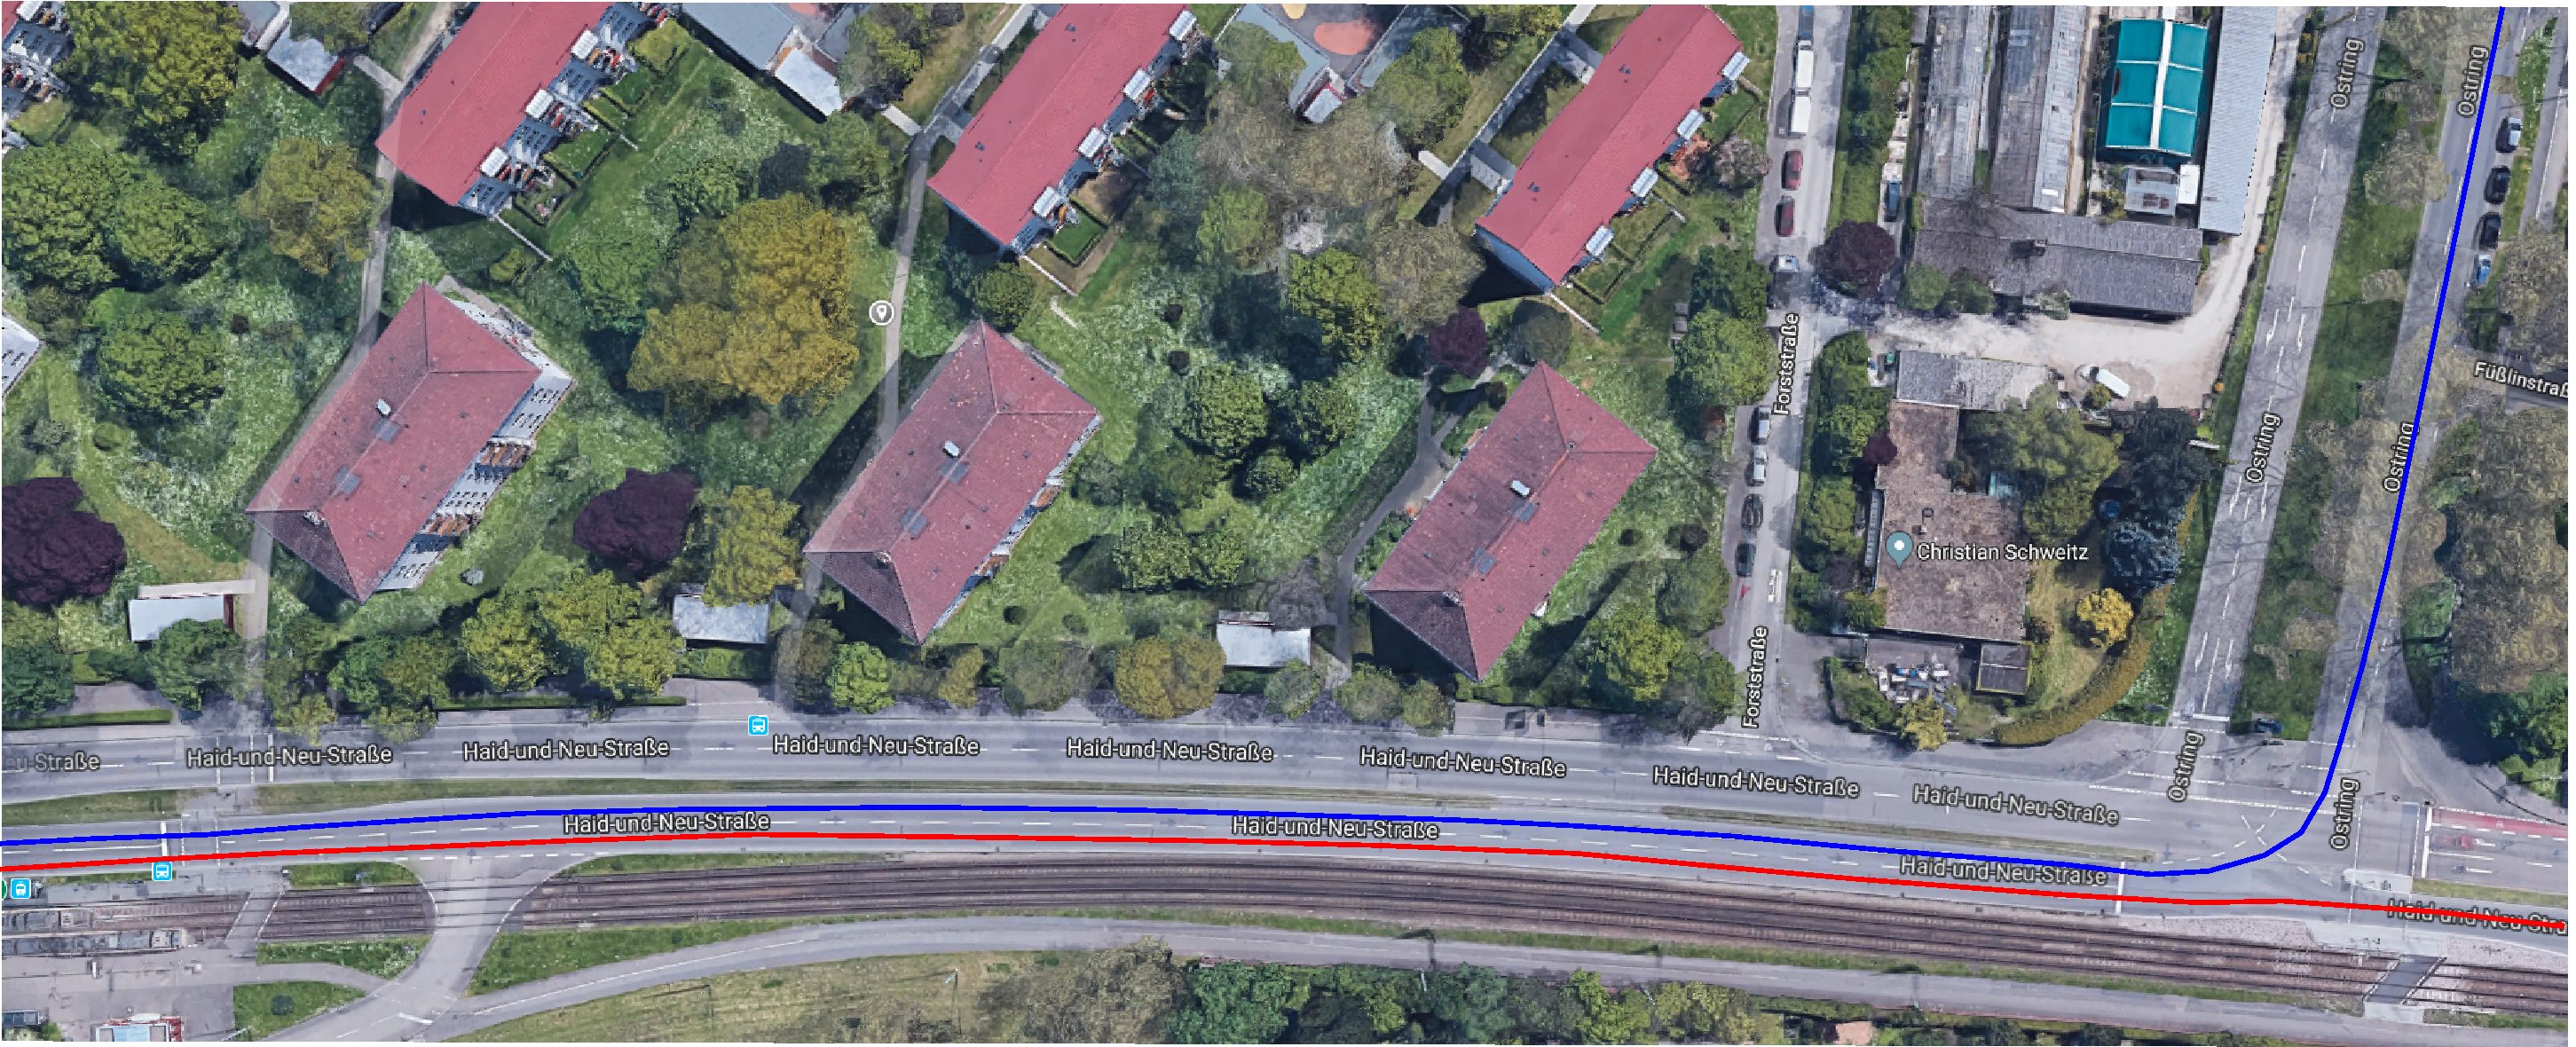
\includegraphics[width =  0.85 \textwidth]{maps.pdf}
        \label{google}
    }
    \subfigure[Darstellung der Haid"=und"=Neu"=Stra{\ss}e in der Simulationsumgebung \gls{ros} basierend auf den Datengrundlagen des Open"=Source"=Karten"=Framework lanelet2]{
        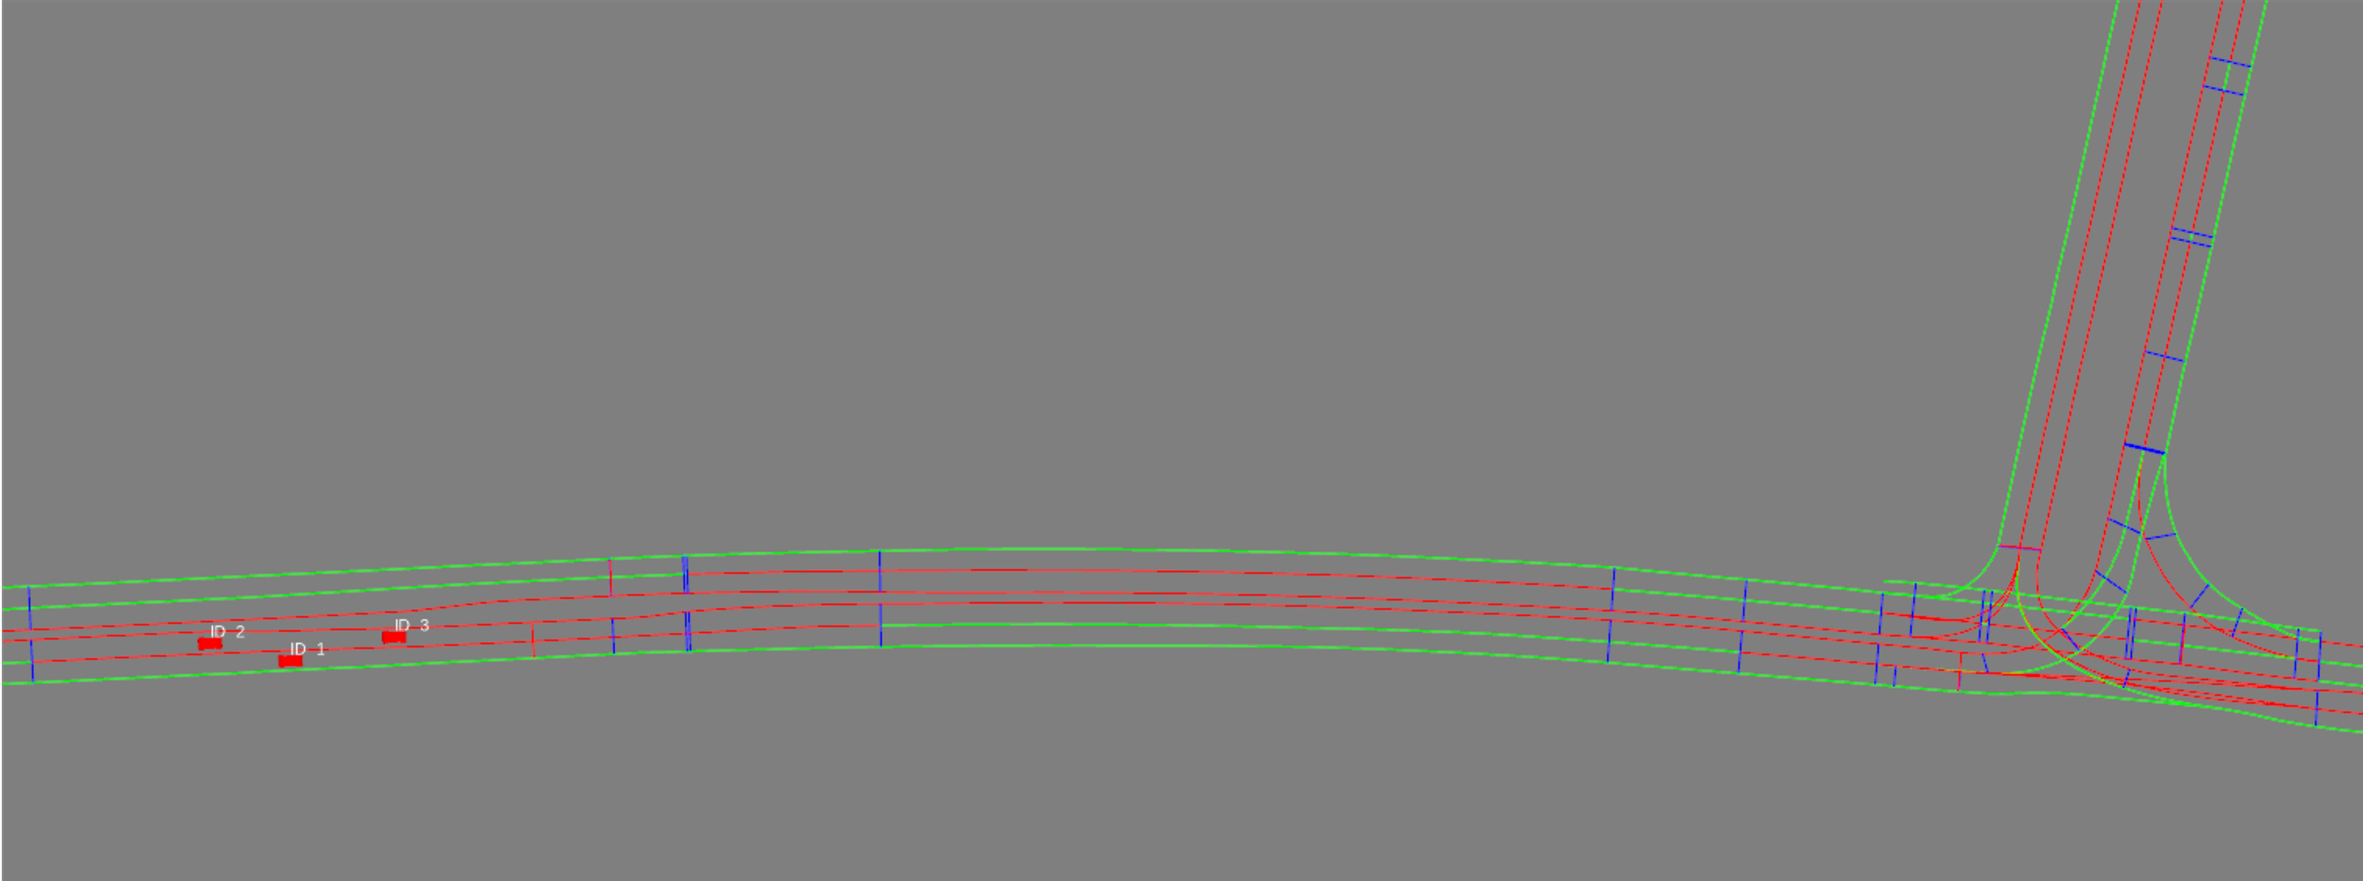
\includegraphics[width =  0.85 \textwidth]{rviz_sce.pdf}
        \label{rviz}
    }
    \caption[Haid-und-Neu"=stra{\ss}e]{Haid"=und"=Neu"=Stra{\ss}e in Karlsruhe}
    \label{fig:Szene}
\end{figure}


\section{Implementierung}
Die Implementierung des Ansatzes fand in der Programmiersprache Python statt.
Der implementierte Ansatz wurde dann in einer \gls{ros}"=Simulationsumgebung eingebunden.
Stra{\ss}eninformationen wie der Verlauf der Referenzkurve und der Fahrstreifen wurden dem von Poggenhans et al. \cite{Poggenhans2018} vorgestelltem Open"=Source"=Karten"=Framework lanelet2 entnommen.
Die Implementierung fand ausschlie{\ss}lich f\"ur die ausgew\"ahlten Szenarien statt.
Teilaspekte die f\"ur die Szenarien nicht relevant sind wurden ausgelassen.
So fand beispielsweise keine Implementierung eines zweifachen Fahrstreifenwechsels oder einer Pfadplanung f\"ur einen freiwilligen Fahrstreifenwechsel statt.
Es wurde bei der Implementierung darauf geachtet, dass der Quellecode modluar aufgebaut ist und somit die entsprechenden Module erg\"anzt werden k\"onnen.
Da der Fokus der Arbeit auf der Konzeptentwicklung liegt, wird im Folgenden nur eine kurze \"Ubersicht zur Implementierung gegeben.


\subsection{Objektorientierte Programmierung}
\label{sec:Objektorientiert}
Die Implementierung in Python fand objektorientiert statt.
Dies tr\"agt zur \"Ubersichtlichkeit des Quellcodes bei und sorgt daf\"ur, dass einzelne Modul leicht ausgetauscht werden k\"onnen.
Es wurden sowohl Klassen zur Beschreibung einzelner Simulationsemelemte als auch f\"ur einzelne Teilschritte des Planungsalgorihmus erstellt.

Klassen zur Beschreibung einzelner Simulationselemente:
\begin{itemize}
\item \textit{Vehicle}: Beschreibung der in der Simulation betrachteten Fahrzeuge. 
Es werden sowohl Informationen \"uber die geometrischen Abmessungen als auch \"uber den Anfangszustand des Fahrzeuges gegeben. 
Jedes Fahrzeug enth\"alt zus\"atzlich ein Objekt der Costfunctional"=Klasse. 
Durch dieses Objekt ist das fahrzeugspezifische Kostenfunktional gegeben.

\item \textit{StreetInfo}: Enth\"alt den Verlauf der Referenzkurve, sowie des aktuellen Fahrstreifens und des Zielfahrstreifens. 
Der aktuelle Fahrstreifen und der Zielfahrstreifen werden durch ein Objekt der Klasse Path beschrieben.
Es werden aus au{\ss}erdem die Informationen gegeben, ab welcher Wegstrecke \gls{symb:s_cs} entlang der Referenzkurve ein Fahrstreifenwechsel eingeleitet werden kann und bis zu welcher Wegstrecke \gls{symb:s_ce} er vollzogen sein muss.

\item \textit{Path}: Geometrische Beschreibung des Verlaufs des Pfades in Frenetkoordinaten.
Die Klasse enth\"alt au{\ss}erdem eine Methode zur Berechnung der Bewegung entlang der Referenzkurve bei gegebener Geschwindigkeit und Beschleunigung des Fahrzeuges.

\item \textit{Costfuntional}: Beschreibung des fahrzeugspezifischen Kostenfunktionals. 
Die Klasse enth\"alt f\"ur jeden Kostenterm (\gls{symb:G_v}, \gls{symb:G_a}, \gls{symb:G_sd}, \gls{symb:G_lc}, \gls{symb:G_lcend}) eine Methoden zur Berechnung der entsprechenden Kosten.
Hier konnte eine bereits vorhandene Klasse erweitert werden.
\end{itemize}

Klassen f\"ur einzelne Teilschritte:
\begin{itemize}
\item \textit{EgoIndependentPrediction}: Erzeugung einer vom Ego"=Fahrzeug unabh\"angigen Bewegungspr\"adiktion aller relevanten Fahrzeuge.
Die Pr\"adiktion findet basierende auf vorgegebenen Anfangszust\"anden der Fahrzeuge sowie deren gew\"unschten Optimalgeschwindigkeit statt.


\item \textit{CreateVelocityProfiles}: Erzeugung zuf\"alliger Geschwindigkeitsprofile. 
Basierend auf einem gegebenen Anfangszustand des Fahrzeuges werden zuf\"allige, diskrete Beschleunigungsverl\"aufe und die entsprechenden Geschwindigkeitsverl\"aufe erzeugt.
Dabei werden die Beschleunigungen und Geschwindigkeiten auf vorgegebene Extremwerte begrenzt.
Es konnte auf einer bestehenden Klasse aufgebaut werden.
 
\item \textit{GenerateCooperativeLaneChangeTrajectorySet}: Erzeugung eines Trajektoriensets f\"ur einen kooperativen Fahrstreifenwechsel.
F\"ur jedes Fahrzeug wird eine Trajektorie ermittelt.
Die Trajektorien werden aufgrund eines vorgegebenen Geschwindigkeitprofils des Ego"=Fahrzeuges und einer vom Ego"=Fahrzeug unabh\"angigen Bewegungspr\"adiktion der restlichen Fahrzeuge ermittelt.
Die Klasse enth\"alt jeweils ein Objekt der Klassen PlanLaneChangePath, Classification und InnerOptimization.

\item \textit{PlanLaneChangePath}: Ermittlung des Pfades f\"ur einen Fahrstreifenwechsel.
Der Pfad ergibt sich aus dem Pfad des aktuellen Fahrstreifens, dem Pfad des Zielfahrstreifens und dem Fahrstreifenwechselpfad.
Der sich ergebende Pfad wird \"uber ein Objekt der Klasse Path beschrieben.
Die Klasse enth\"alt au{\ss}erdem die Information zu welchem Zeitpunkt \(t_\mathrm{lc, start}\) der Fahrstreifenwechsel eingeleitet wird, zu welchem Zeitpunkt \gls{symb:t_lc} das Fahrzeuge auf den Zielfahrstreifen auff\"ahrt und zu welchem Zeitpunkt \(t_\mathrm{lc, end}\) der Fahrstreifenwechsel beendet wird.

\item \textit{Classification}: Klassifizierung der Fahrzeuge. 
Die Fahrzeuge werden aufgrund der vom Ego"=Fahrzeug unabh\"angigen Bewegungspr\"adiktion und einer gegeben Trajektorie des Ego"=Fahrzeuges in beteiligte, unbeteiligte und beeinflusste Fahrzeuge eingeteilt.

\item \textit{InnerOptimization}: Ermittlung einer kooperativen Fahrstreifenwechseltrajektorie eines beteiligten Fahrzeuges bei gegebener Trajektorie des Ego"=Fahrzeuges. 
Die L\"osung des inneren Optimierungsproblems findet durch einen samplingbasierten Ansatz statt, bei dem randomisierte Geschwindigkeitsprofile erzeugt werden.
Dazu wird ein Objekt der Klasse CreateVelocityProfiles erzeugt.


\end{itemize}

\subsection{Erzeugung randomisierter Geschwindigikeitsprofil}
Die Erzeugung der randomisierten Geschwindigkeitsprofile findet in der in Kapitel~\ref{sec:Objektorientiert} vorgestellten Klasse CreateVelocityProfiles statt.
Dabei wird f\"ur jeden einzelnen Zeitschritt einer Trajektorie ein zuf\"alliger Ruck aus einer beschr\"ankten Menge generiert.
Durch numerische Integration werden daraus diskretisierte Beschleunigungs- und Geschwindigkeitsverl\"aufe berechnet.
In Abbildung~\ref{fig:Geschwindgkeitsprofile} ist das Ergebnis von 1000 zuf\"allig ermittelten Geschwindigkeitsprofilen dargestellt.

Wie in Kapitel~\ref{sec:SmapPVD} beschrieben wird bei der Ermittlung eines zuf\"alligen Geschwindigkeitsprofils die Beschleunigung und die Geschwindigkeit durch einen Maximal- und einen Minimalwert begrenzt.
Dazu werden zuerst ohne Beachtung dieser Grenzwerte die Beschleunigungen und Geschwindigkeiten aus den zuf\"alligen R\"ucken berechnet.
Anschlie{\ss}end wird gepr\"uft, bei welchem Geschwindigkeitsprofil ein Grenzwert \"uberschritten wird. 
Wird ein Beschleunigungsgrenzwert \"uberschritten, wird der entsprechende Wert auf den Grenzwert gesetzt.
Wird ein Geschwindigkeitsgrenzwert \"uberschritten, wird der entsprechende Wert auf den Grenzwert gesetzt und es wird auf den entsprechenden Beschleunigungswert aus dem Zeitschritt davor zur\"uckgerechnet.
Dieser wird dann so angepasst, dass er zu dem neu gesetzten Geschwindigkeitswert f\"uhrt.

Diese Vorgehen hat einige Vorteile gegen\"uber dem Vorgehen, dass bei der Erzeugung des Rucks bereits die Menge aus dem das Sample erzeugt wird so begrenzt wird, dass die Grenzwerte nicht \"uberschritten werden:

 \begin{itemize}
 
 \item Es k\"onnen alle R\"ucke aus einer vorher festgelegten beschr\"ankten Menge erzeugt werden.
Damit kann auf sehr effiziente Verfahren zur Erzeugung von Matritzen mit zuf\"alligen Werte zur\"uckgegriffen werden.

\item Es m\"ussen nicht f\"ur jeden Ruck einzeln die Grenzwerte die sich aus den Beschleunigungs- und Geschwindigkeitsgrenzwerten ergeben berechnet werden.
Eine Berechnung findet nur da statt, wo auch wirklich ein Grenzwert \"uberschritten wird.
F\"ur diese \"Uberpr\"ufung k\"onnen ebenfalls sehr effiziente Verfahren genutzt werden.

\item Die Geschwindigkeitsprofile sind nicht normalverteilt, sondern es entsteht eine Anh\"aufung an den Randbereichen des zul\"assigen Bereichs. 
 Dies wird als positiv gewertet, da erwartet wird, dass sich die L\"osung des Optimierungsproblems oft in den Randbereichen befindet.
 
 \end{itemize} 
 
 
\begin{figure}[!htbp]
    \centering
    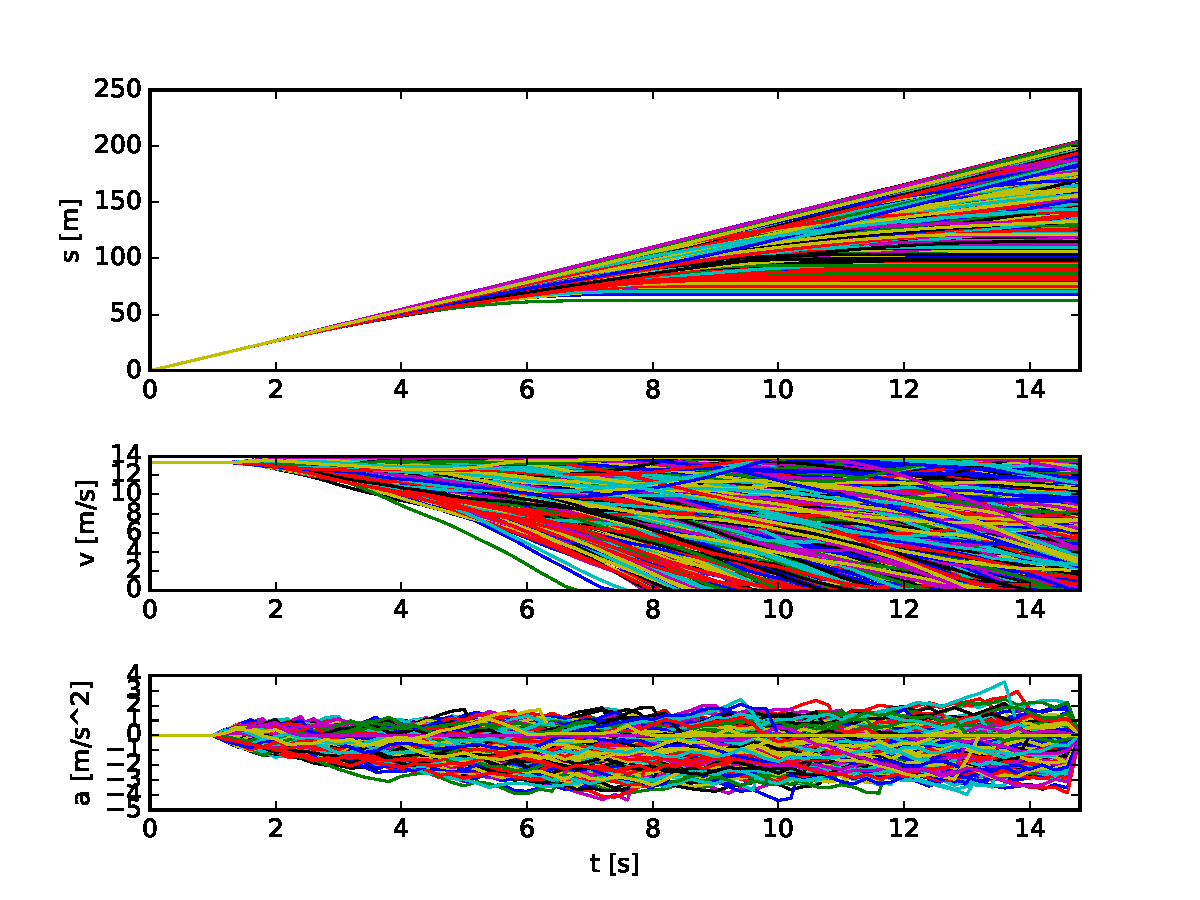
\includegraphics[width = 0.7 \textwidth ]{Geschwindigkeitsprofile.pdf}
    \caption[Erzeugung von Geschwindigkeitsprofilen]{Darstellung von 1000 zuf\"allig ermittelten Geschwindigkeitsprofilen. In der ersten Sekunde stimmen alle Geschwindigkeitsprofile \"uberein, da hier die Trajektorie aus dem vorausgegangen Planungsschritt \"ubernommen wird.}
    \label{fig:Geschwindgkeitsprofile}
\end{figure}


\subsection{Berechnung der normalisierten Sicherheitsabst\"ande}
Wie in Kapitel~\ref{sec:LCKostfunc} beschrieben werden zur Berechnung des Kostentermes \gls{symb:G_sd} normalisierte Sicherheitsabst\"ande \gls{symb:d_normal} berechnet.
Die Berechnung der normalisierten Sicherheitsabst\"ande findet an den diskreten Zeitschritten statt.
Es wurde drauf verzichtet, diese Abst\"ande ausschlie{\ss}lich f\"ur das Fahrzeug, das sich direkt vor dem Ego"=Fahrzeug auf dem selben Fahrstreifen befindet, zu berechnen.
Vielmehr wurden bei der Berechnung alle Fahrzeuge der Simulation betrachtet.
Damit ist gew\"ahrleistet, dass die fahrstreifenbasierte Pr\"adiktion durch eine komplexere Pr\"adiktion ausgetauscht werden kann, ohne dass die Berechnung der normalisierten Sicherheitsabst\"ande neu implementiert werden muss.
Eine komplexere Pr\"adiktion k\"onnte auch Fahrstreifenwechselintensionen von anderen Fahrzeugen ber\"ucksichtigen.

Um den Rechenaufwand nicht unn\"otig zu steigern wurde eine Filterfunktion eingebaut.
Diese schlie{\ss}t Fahrzeuge die sich an einem diskreten Zeitpunkt hinter dem betrachteten Fahrzeug oder weit vor diesem befinden von der Ber\"ucksichtigung aus.


\subsection{Anpassung des \gls{idm}}
Die in Kapitel~\ref{sec:IDMpred} vorgestellte Formel des \gls{idm} zur Berechnung eines Geschwindigkeitsprofiles f\"ur ein Fahrzeug in Folgefahrt sorgt f\"ur ein nicht zufriedenstellendes Fahrverhalten.
Es wurden deshalb folgende Anpassungen vorgenommen:

\begin{itemize}


\item \textit{Begrenzung des Rucks}: Ein hoher Ruck wird von Fahrzeuginsassen als besonders unangenehm empfunden. 
Bei der Berechnung der Beschleunigungswerte werden diese deshalb so begrenzt werden, dass sowohl ein negativer als auch positiver Grenzwert (\(j_\mathrm{min}\) und \(j_\mathrm{max}\)) des Rucks nicht \"uberschritten wird.

\item \textit{Ausschlu{\ss} von negativen Geschwindigkeiten}: Es wird davon ausgegangen, dass bei einem normalen Fahrstreifenwechselman\"over keines der beteiligten Fahrzeuge r\"uckw\"arts f\"ahrt.
Deshalb wird bei der Berechnung der Beschleunigung eine minimal zul\"assige Beschleunigung berechnet, bei der das Fahrzeug zum Stillstand kommen w\"urde.

\item \textit{Abschnittsweise Unterdr\"uckung des interaktiven Terms}: Der interaktive Term sorgt daf\"ur, dass selbst bei gro{\ss}em Abstand zum Vorderfahrzeug die optimale Geschwindigkeit bis zum n\"achsten Abtastzeitpunkt nicht konstant gehalten wird.
Der interaktive Term wird deshalb bei gro{\ss}em Abstand zum Vorderfahrzeug unterdr\"uckt.
Erst wenn der Abstand der Fahrzeuge \( s_\alpha < 1.3 s^*\) ist wird der interaktive Term zur Berechnung der Beschleunigung ber\"ucksichtigt.
Der Term \(s^*\) ist der im \gls{idm} berechnete Wunschabstand des Folgefahrzeuges zum vorderen Fahrzeug (vgl. Kapitel~\ref{sec:IDMpred}).

\end{itemize}



\section{Auswertung}

In diesem Abschnitt werden die Simulationsergebnisse vorgestellt und diskutiert.
Eine eindeutige Aussage \"uber die Qualit\"at eines Trajektorienplanungsansatzes zu Treffen ist nur sehr schwer m\"oglich.
Die Bewertung anhand eines Kostenfunktionals h\"angt stark von dem gew\"ahlten Kostenfunktional ab.
Dieses Kostenfunktional soll daf\"ur sorgen, dass es zu keiner Kollision mit Hindernissen oder anderen Verkehrsteilnehmern kommt.
Weiter noch soll es zu einer Trajektorie f\"uhren die von den Insassen als m\"oglichst angenehm empfunden wird.
Dieses Empfinden h\"angt stark von der betreffenden Person ab.
Entsprechend muss das Kostenfunktional, um die tats\"achlich optimale Trajektorie zu ermitteln, auf die Person angepasst sein.
Eine konkrete Aussage \"uber die Qualit\"at einer Trajektorie anhand der Kosten ist dementsprechend immer nur f\"ur eine bestimmt Person zul\"assig.

Es lassen sich jedoch qualitative Aussagen treffen.
So sollten in der Regel hohe R\"ucke und Beschleunigungen vermieden werden.
Zus\"atzlich sollte das Fahrzeug mit einer Geschwindigkeit fahren die m\"oglichst nah an einer gew\"unschten optimalen Geschwindigkeit liegt und Abst\"ande zu anderen Fahrzeugen sollten nicht zu gering sein.
In der Regel ist es nicht m\"oglich alle Aspekte komplett zu erf\"ullen.
Die einzelnen Kostenterme spiegeln wider wie stark die Trajektorie von den Optimalwerten abweicht.

Eine weitere Schwierigkeit besteht darin, dass bei diesem Ansatz ein Trajektorienset gefunden werden soll, bei dem die Interaktion mit anderen Fahrzeugen ber\"ucksichtigt wird.
Daf\"ur muss pr\"adiziert werden, wie andere Fahrzeuge auf das eigene Fahrverhalten reagieren werden.
Die Reaktion der Fahrzeuge Testdaten zu entnehmen ist kaum m\"oglich.
Zum einen m\"ussten dadurch auch sicherheitskritische Situationen getestet werden.
Zum anderen ist die Reaktion sehr personenspezifisch und spiegelt nur eine von vielen m\"oglichen Reaktionen wieder.
Laut Naumann et al. \cite{Naumann2018} gibt es drei M\"oglichkeiten warum ein Fahrzeug von der vorhergesagten Trajektorie abweicht:
\begin{itemize}
\item Das Kostenfunktional oder das Ziel des betreffenden Fahrzeuges wurde falsch eingesch\"atzt.
\item Das Fahrzeug hat das Kostenfunktional des Ego"=Fahrzeuges falsch eingesch\"atzt.
\item Das Fahrzeug verh\"alt sich nicht entsprechend der angenommenen Verhaltenspolitik.
\end{itemize}
F\"ur eine pr\"azise Pr\"adiktion m\"usste also das Kostenfunktional des interagierenden Fahrzeuges bekannt sein.
Dies ist in der Regel nicht der Fall.
Ist es bekannt, ist dennoch nicht sichergestellt, ob sich das Fahrzeug dementsprechend verhalten wird.
 
Bei der Evaluierung des Ansatzes soll deshalb zuerst davon ausgegangen werden, dass andere Fahrzeuge sich entsprechend der vom Ansatz generierten Bewegungspr\"adiktion verhalten.
Es werden zun\"achst die Ergebnisse eines einzelnen Planungsschrittes betrachte.
Anschlie{\ss}end wird der Ansatz bei einer fortlaufenden Neuplanung untersucht.
Dabei soll zuerst von einem kooperativen Verhalten der anderen Verkehrsteilnehmer ausgegangen werden.
Anschlie{\ss}end wird untersucht wie das Ego"=Fahrzeug durch den vorgestellten Ansatz auf ein egoisitisches Verhalten der anderen Verkehrsteilnehmer reagiert.

Zur Beurteilung der sich ergebenden Trajektoriensets k\"onnen folgende Fragen genutzt werden:
\begin{itemize}
\item Wird ein kooperatives Verhalten der Verkehrsteilnehmer widergespiegelt?
\item Werden kollisionsfreie Trajektorien generiert?
\item Werden Sicherheitsabst\"ande eingehalten?
\item Wie stark sind die Abweichungen der einzelnen Fahrzeuge von den angenommenen Wunschgeschwindigkeiten?
\item Wie hoch sind die Beschleunigungen der betrachteten Fahrzeuge?
\end{itemize}


In den Simulationen wurde f\"ur jedes Fahrzeug das gleich Kostenfunktional angenommen.
Die entsprechenden Parameter sind in Tabelle~\ref{tab:Kostfunc} im Anhang gegeben. 
In einzelnen F\"allen weicht das Kostenfunktional des Ego"=Fahrzeuges von diesen Parametern ab.
Ist dies der Fall wird darauf hingewiesen und die Abweichung begr\"undet.

Die Fahrzeuge auf dem Zielfahrstreifen werden zum Zweck einer eindeutigen Beschreibung durchnummeriert.
Das vorderste Fahrzeug auf dem Zielfahrstreifen wird als Fahrzeug 2 bezeichnet.
Die Fahrzeug dahinter werden aufsteigend bis zum hintersten Fahrzeug durchnummeriert.

\subsection{Einzelner Planungsschritt}
\label{sec:einzelPlanungsschritt}
Es sollen zun\"achst die Ergebnisse eines einzelnen Planungsschrittes betrachtet werden.
Die Ergebnisse zeigen jeweils die erzeugte Trajektorie des Ego"=Fahrzeuges und die kooperative Bewegungspr\"adiktion der anderen Fahrzeuge.
Nur f\"ur den Fall, dass sich alle Fahrzeuge entsprechend diesem Trajektorienset verhalten entspricht dies auch dem letztentlich gefahrenen Trajektorienset.
Dies ist in der Regel nicht der Fall.
Es werden deshalb sowohl eine Neuplanung als auch Sicherheits\"uberpr\"ufungen notwendig.
Trotzdem ist es sinnvoll zun\"achst die Ergebnisse eines einzelnen Planungsschrittes zu analysieren um grundlegende Aussagen \"uber den Planungsansatz treffen zu k\"onnen.
Der in dieser Arbeit vorgestellte Ansatz wurde in verschiedenen Szenarien getestet.
Die verschiedenen Szenarien und repr\"asentativen Simulationsergebnisse der Szenarien werden im Folgenden vorgestellt.


\minisec{Zwei Fahrzeuge auf dem Zielfahrstreifen}
Im ersten Szenario befinden sich zwei Fahrzeuge auf dem Zielfahrstreifen.
Das Ego"=Fahrzeug befindet sich auf dem Fahrstreifen rechts neben den beiden Fahrzeugen und in lateraler Richtung zwischen den beiden Fahrzeugen.
Der Abstand zwischen den Fahrzeugen 2 und 3 ist anf\"anglich so gro{\ss}, dass kein weiteres Fahrzeug zwischen ihnen auf den Zielfahrstreifen auffahren kann, ohne dass Sicherheitsabst\"ande deutlich unterschritten werden.
Die Anfangsgeschwindigkeit der Fahrzeuge entspricht ihrer Optimalgeschwindigkeit und ist so gew\"ahlt, dass das Ego"=Fahrzeug bei einer egoistischen Planung zwischen den Fahrzeugen auf den Zielfahrstreifen auffahren w\"urde.
Eine sichere Fahrstreifenwechseltrajektorie kann deshalb nur gefunden werden, wenn mindestens eines der Fahrzeuge von seiner Optimalgeschwindigkeit abweicht.
Die Ausgangsposition ist in Abbildung~\ref{fig:two_veh_scene} dargestellt.
Die Startzust\"ande der Fahrzeuge sind in Tabelle~\ref{tab:StartS1} gegeben.
 
\begin{figure}[!htbp]
    \centering
    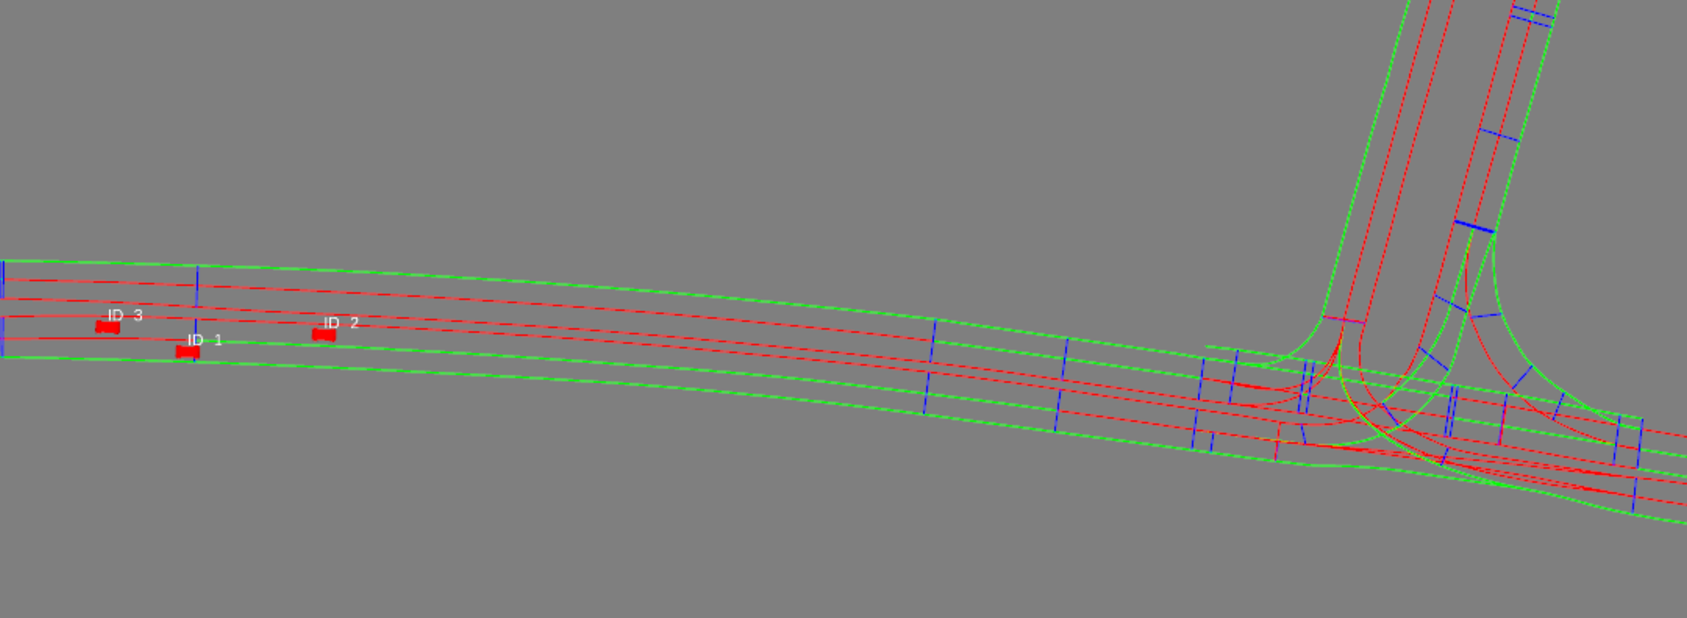
\includegraphics[width = 0.8 \textwidth ]{two_veh_sce.pdf}
    \caption[Szenario 1]{Ausgangsposition der Fahrzeuge im ersten Szenario}
    \label{fig:two_veh_scene} 
\end{figure}

\sisetup{round-mode = places, round-precision = 2, scientific-notation = fixed, fixed-exponent = 0}
\begin{table}[!htbp]
    \centering
    \begin{tabular}{crSSSS}
        \hline
        & & {\gls{symb:a_start}  [m/s\textasciicircum 2]} & {\gls{symb:v_start} [km/h]} & {\gls{symb:v_opt} [km/h]} & {Abstand zu   \gls{symb:s_cmax} [m]} \\%
        \hline
        & Ego"=Fahrzeug & 00.00e+00 & 48.00e+00 & 48.00e+00 & 108.65e+00\\
        & Fahrzeug 2 & 00.00e+00 & 48.00e+00 & 48.00e+00 & 86.74e+00\\
        & Fahrzeug 3 & 00.00e+00 & 48.00e+00 & 48.00e+00 & 121.71e+00\\
         \hline
    \end{tabular}
    \caption[Startzust\"ande Szenario 1]{Startzust\"ande der Fahrzeuge im ersten Szenario.
    }\label{tab:StartS1}
\end{table}

Das Ergebnis eines einzelnen Planungsschrittes ist in Abbildung~\ref{zweiFahrzeugeKoop} dargestellt.
Das Ego"=Fahrzeug ordnet sich zwischen den beiden Fahrzeugen auf dem Zielfahrstreifen ein.
Beide Fahrzeuge auf dem Zielfahrstreifen zeigen ein kooperatives Verhalten.
Das vordere Fahrzeug (Fahrzeug 2) f\"ahrt bereits sehr nahe an der maximalen Geschwindigkeit.
Deshalb ist das kooperative Verhalten nicht stark ausgepr\"agt.
Es ist lediglich ein leichtes Erh\"ohen der Geschwindigkeit zu erkennen.
Das Ego"=Fahrzeug senkt seine Geschwindigkeit bis zum Fahrstreifenwechsel leicht ab um den entsprechenden Sicherheitsabstand zum vorderen Fahrzeug beim Auffahren auf den Zielfahrstreifen einzuhalten.
Anschlie{\ss}end beschleunigt es um sich wieder seiner Optimalgeschwindigkeit anzun\"ahern.
Beim hinteren Fahrzeug auf dem Zielfahrstreifen (Fahrzeug 3) ist eindeutiges kooperatives Verhalten zu erkennen.
Es weicht von seiner Optimalgeschwindigkeit ab um dem Ego"=Fahrzeug das Auffahren auf den Zielfahrstreifen zu erleichtern.
Der laterale Abstand zwischen den beiden Fahrzeugen w\"achst ab dem Zeitpunkt, ab dem die Fahrstreifenwechselintension erkannt wird, bis zum Fahrstreifenwechsel kontinuierlich an.
Sobald sich das Ego"=Fahrzeug auf dem Zielfahrstreifen befindet geht Fahrzeug 3 in die Folgefahrt \"uber und f\"angt an seine Geschwindigkeit wieder zu erh\"ohen.
Gegen Ende des Planungshorizontes haben sich alle Fahrzeuge wieder ihrer Optimalgeschwindigkeit angen\"ahert und es haben sich nahezu gleichm\"a{\ss}ige Abst\"ande zwischen den Fahrzeugen gebildet.

Zum Vergleich ist in Abbildung~\ref{zweiFahrzeugeEgo} das Ergebnis dargestellt, wenn von einem egoistischen Verhalten der Fahrzeuge auf dem Zielfahrstreifen ausgegangen wird.
Hierzu wurden zuf\"allige Trajektorien des Ego"=Fahrzeuges generiert.
Die Fahrzeuge auf dem Zielfahrstreifen behalten ihre Geschwindigkeit bei.
Ihre Trajektorie ist somit vorgegeben.
Anschlie{\ss}end wird jede generierte Trajektorie des Ego"=Fahrzeuges mit den vorgegebenen Trajektorien der Fahrzeuge auf dem Zielfahrstreifen kombiniert und das sich ergebende Trajektorienset anhand des Kostenfunktionals bewertet.
Zur Generierung der zuf\"alligen Trajektorien des Ego"=Fahrzeuges wurde der selbe Algorithmus verwendet wie in der kooperativen Simulation in der von einem kooperativen Verhalten der anderen Fahrzeuge ausgegangen wird. 
Die Bewertung der Trajektorie fand mit dem gleiche Kostenfunktional.

Bei einem egoistischen Verhalten der Fahrzeuge auf dem Zielfahrstreifen ist das Ego"=Fahrzeug gezwungen diese zuerst passieren zu lassen.
Dazu muss es deutlich von seiner Optimalgeschwindigkeit abweichen.
Die minimale Geschwindigkeit des Ego"=Fahrzeuges ist deutlich geringer als bei der Annahme eines kooperativen Verhaltens.
Erst wenn die Fahrzeuge auf dem Zielfahrstreifen vorbeigefahren sind kann das Ego"=Fahrzeug wieder beschleunigen und auf den Zielfahrstreifen auffahren.

Die einzelnen Kostenterme der beiden Szenarien sind in Tabelle~\ref{tab:Kostenvergleich} gegen\"ubergestellt.
Ein Vergleich der Kostenterme spiegelt die gemachten Beobachtungen wieder.
Der Geschwindigkeitsterm \gls{symb:G_v} des Ego"=Fahrzeuges konnten durch ein kooperatives Verhalten der Fahrzeuge auf dem Zielfahrstreifen deutlich herabgesetzt werden.
Auch die Kostenterme \gls{symb:G_a} und \gls{symb:G_sd}  fallen geringer aus.
Im Gegenzug kommen bei den Gesamtkosten Kosten f\"ur das kooperative Fahrzeug hinzu.
Doch auch hier spiegelt der Geschwindigkeitsterm wider, dass das Fahrzeug wesentlich weniger von seiner Optimalgeschwindigkeit abweichen muss als das Ego-Fahrzeug bei einem unkooperativen Fahrstreifenwechsel.
Insgesamt konnten die Kosten basierend auf dem verwendeten Kostenfunktional um \(47.43\%\) gesenkt werden.

\begin{figure}[!htbp]
    \centering
    \subfigure[Kooperativ ]{
        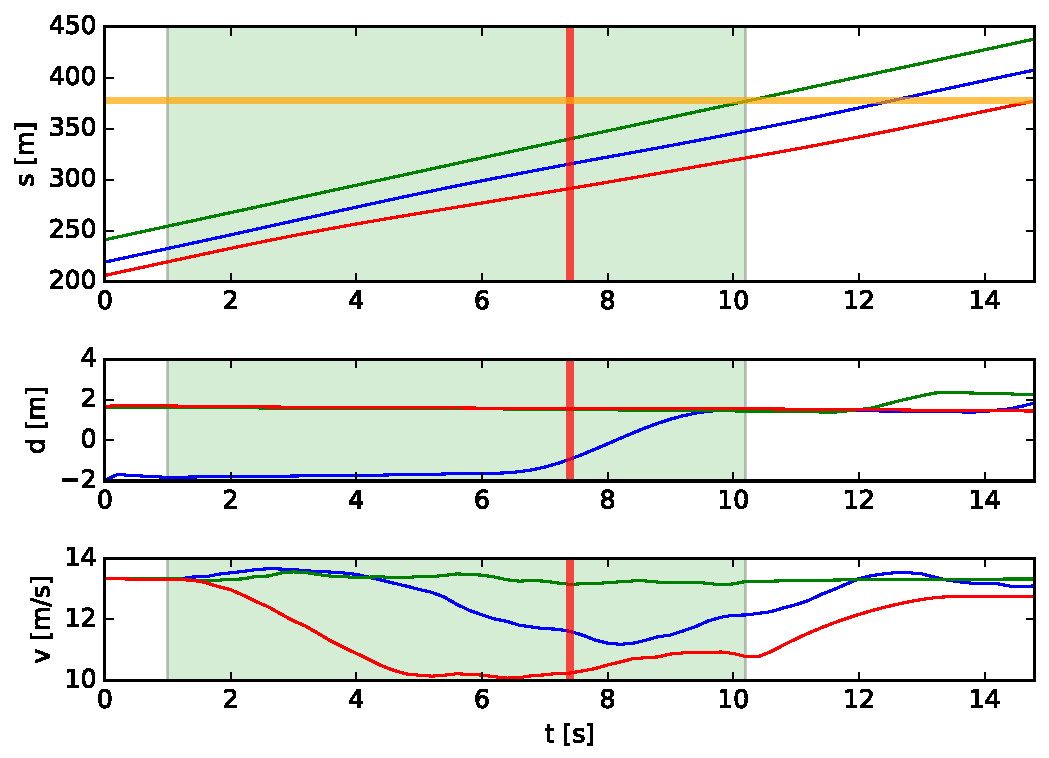
\includegraphics[width =  0.8 \textwidth]{two_veh_result.pdf}
        \label{zweiFahrzeugeKoop}
    }
    \subfigure[Unkooperative]{
        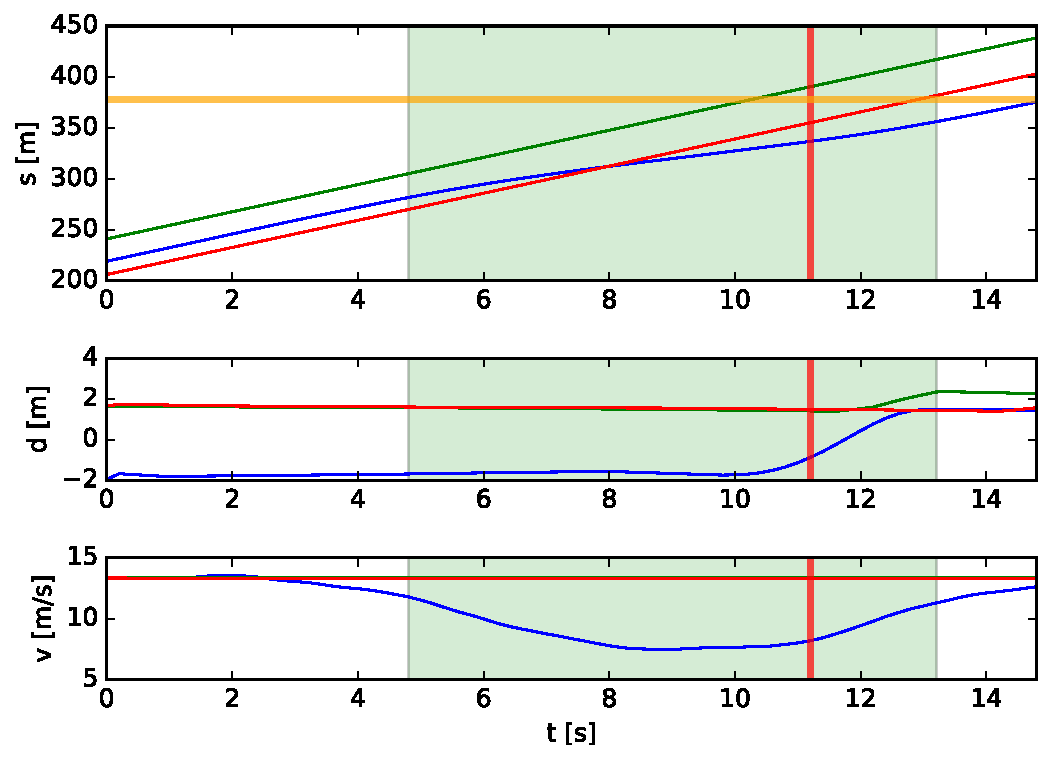
\includegraphics[width = 0.8  \textwidth]{two_veh_ego_result.pdf}
        \label{zweiFahrzeugeEgo}
    }
    \caption[Fahrstreifenwechsel Vergleich]{Vergleich von einem kooperativen und einem unkooperativen Fahrstreifenwechsel. 
    Das Ego"=Fahrzeug ist durch die blaue Line gekennzeichnet die restlichen Fahrzeuge befinden sich auf dem Zielfahrstreifen.
    Der Zeitbereich von \gls{symb:t_coop,start} bis \gls{symb:t_coop,end} ist gr\"un hinterlegt. Die vertikale rote Line kennzeichnet den Zeitpunkt des Fahrstreifenwechsels \gls{symb:t_lc}. Die orange horizontale Line kennzeichnet bis zu welcher Wegstrecke \gls{symb:s_cmax} der Fahrstreifenwechsel beendet sein muss.
    (Am Ende des Planushorizonts ist ein Anstieg von \gls{symb:d_r} zu sehen nach dem der Fahrstreifenwechsel durchgef\"uhrt wurde. Dies liegt daran, das hier der Pfad des Zielfahrstreifens st\"arker von der Referenzkurve abweicht. Die Fahrzeuge befinden sich noch immer auf dem Zielfahrstreifen)}
    \label{fig:Vergleich}
\end{figure}


\sisetup{round-mode = places, round-precision = 2, scientific-notation = fixed, fixed-exponent = 0}
\begin{table}[!htbp]
    \centering
    \begin{tabular}{crSSSSS|S}
        \hline
        & & \textbf{\gls{symb:G_a}} & \textbf{\gls{symb:G_v}} & \textbf{\gls{symb:G_sd}} & \textbf{\gls{symb:G_lc}} & \textbf{\gls{symb:G_lcend}} & {Fahrzeugkosten}\\%
        \hline
        & Ego"=Fahrzeug & 15.13e+00 & 8.30e+00 & 0.00e+00 & 0.0e+00 & x & 23.43e+00\\
        & Fahrzeug 2 & 1.76e+00 & 0.11e+00 & 0.0e+00 & 0.0e+00 & 0.19e+00 & 2.06e+00\\
        & Fahrzeug 3 & 21.96e+00 & 37.37e+00 & 0.09e+00 & 0.0e+00 & 10.46e+00 & 69.88e+00\\
        & Multi-Agenten & 38.85e+0 & 45.78e+00 & 0.09e+00 & 0.0e+00 & 10.65e+00 & 95.37e+00\\
        \hline
        &  Egoistische Pr\"adiktion& 61.09e+00 & 115.40e+00 & 4.91e+00 & 0.00e+00 & x & 181.40e+00\\
         \hline
    \end{tabular}
    \caption[Kostenvergleich]{Vergleich der Kosten eines kooperativen Fahrstreifenwechsels ermittelt durch eine Multi-Agenten-Optimierung und eines unkooperativen Fahrstreifenwechsels.
    }\label{tab:Kostenvergleich}
\end{table}



\minisec{Vier Fahrzeuge auf dem Zielfahrstreifen}
Im ersten Szenario konnte gezeigt werden, dass durch den vorgestellten Ansatz ein kooperatives Verhalten der Fahrzeuge auf dem Zielfahrstreifen widergespiegelt werden kann.
Im Vergleich dazu ist das Ego"=Fahrzeug bei einem egoistischen Verhalten der anderen Verkehrsteilnehmer gezwungen deutlich st\"arker von seiner Optimalgeschwindigkeit abzuweichen.
Es kann den Fahrstreifenwelchsel jedoch auch ohne kooperatives Verhalten der anderen Verkehrsteilnehmer durchf\"uhren, ohne dabei auf dem aktuellen Fahrstreifen anzuhalten.
Im Folgenden soll nun \"ahnliche Szenarien untersucht werden, wobei sich jedoch vier Fahrzeuge auf dem Fahrstreifen befinden.
Damit soll eine dicht befahrene Stra{\ss}e dargestellt werden.
Der Abstand zwischen den Fahrzeugen auf dem Zielfahrstreifen ist anf\"anglich wieder so gew\"ahlt, dass die L\"ucken nicht gro{\ss} genug f\"ur einen sicheren Fahrstreifenwechsel sind.
Die Ausgangspositionen der Fahrzeuge sind in Abbildung~\ref{fig:four_veh_scene} dargestellt.
Zuerst wird in Szenario 2.1 \"ahnlich zum ersten Szenario angenommen, dass das Ego"=Fahrzeug die gleiche Geschwindigkeit wie die Fahrzeuge auf dem Zielfahrstreifen hat.
In den Szenarien 2.2, 2.3 und 2.4 wird dann die Geschwindigkeit des Ego-Fahrzeuges variiert.
Es wird angenommen, dass die niedrigere Anfangsgeschwindigkeit nicht durch Interaktion mit anderen Fahrzeugen verursacht wurde.
Deshalb ist nicht davon auszugehen das die Anfangsgeschwindigkeit bereits im diskomfortablen Bereich liegt.
Das Kostenfunktional des Ego"=Fahrzeuges wird bei den entsprechenden Szenarien deshalb so angepasst, dass der unkomfortable Bereich f\"ur negative Abweichungen von der Optimalgeschwindigkeit unter der Anfangsgeschwindigkeit des Ego"=Fahrzeuges beginnt.
Die Startzust\"ande der Fahrzeuge auf dem Zielfahrstreifen bleiben in allen Szenarien unver\"andert.
Die Anfangszust\"ande der Fahrzeuge f\"ur die verschiedenen Szenarien sind in Tabelle~\ref{tab:StartS2} gegeben.

\begin{figure}[!htbp]
    \centering
    \includegraphics[width = 0.8 \textwidth ]{four_veh_sce.pdf}
    \caption[Szenario 2]{Ausgangsposition der Fahrzeuge in den Szenarien 2.1, 2.2, 2.3, 2.4}
    \label{fig:four_veh_scene} 
\end{figure}


\sisetup{round-mode = places, round-precision = 2, scientific-notation = fixed, fixed-exponent = 0}
\begin{table}[!htbp]
    \centering
    \begin{tabular}{crSSSS}
        \hline
        & & {\gls{symb:a_start}  [m/s\textasciicircum 2]} & {\gls{symb:v_start} [km/h]} & {\gls{symb:v_opt} [km/h]} & {Abstand zu   \gls{symb:s_cmax} [m]} \\%
        \hline
        & Fahrzeug 2 & 00.00e+00 & 48.00e+00 & 48.00e+00 & 86.74e+00\\
        & Fahrzeug 3 & 00.00e+00 & 48.00e+00 & 48.00e+00 & 121.71e+00\\
        & Fahrzeug 4 & 00.00e+00 & 48.00e+00 & 48.00e+00 & 156.65e+00\\
        & Fahrzeug 5 & 00.00e+00 & 48.00e+00 & 48.00e+00 & 191.69e+00\\
         \hline
         & Ego"=F. Sze. 2.1 & 00.00e+00 & 48.00e+00 & 48.00e+00 & 108.65e+00\\
         & Ego"=F. Sze. 2.2 & 00.00e+00 & 40.00e+00 & 48.00e+00 & 108.65e+00\\
         & Ego"=F. Sze. 2.3 & 00.00e+00 & 30.00e+00 & 48.00e+00 & 108.65e+00\\
         & Ego"=F. Sze. 2.4 & 00.00e+00 & 25.00e+00 & 48.00e+00 & 108.65e+00\\
          \hline
    \end{tabular}
    \caption[Startzust\"ande Szenarien 2]{Startzust\"ande der Fahrzeuge f\"ur die Szenarien mit vier Fahrzeugen auf dem Zielfahrstreifen.
    }\label{tab:StartS2}
\end{table}

Im Vergleich zum ersten Szenario werden in den folgenden Szenarien zwei weitere Fahrzeuge in der Simulation in Betracht gezogen.
Die Anzahl der potentiellen kooperativen Partner wurde somit verdoppelt.
Die Simulationen fanden auf dem gleichen Rechner und unter der Nutzung gleich vieler Kerne statt.
Die Rechenzeit ist im Vergleich um lediglich 63\% und damit weniger als linear mit der Anzahl der Fahrzeuge angestiegen.

Die Simulationsergebnisse von Szenario 2.1 sind in Abbildung~\ref{fig:VierFahrzeuge} dargestellt.
Es zeigt sich ein \"ahnliches Verhalten wie im ersten Szenario.
Das Ego"=Fahrzeug f\"ahrt in die L\"ucke zwischen den Fahrzeugen 2 und 3 ein.
Das vorderste Fahrzeug auf dem Zielfahrstreifen (Fahrzeug 2) bleibt von dem Fahrstreifenwechselman\"over weitesgehend unbeeinflusst.
Das zweite Fahrzeug auf dem Zielfahrstreifen (Fahrzeug 3) senkt seine Geschwindigkeit ab um die L\"ucke f\"ur den Fahrstreifenwechsel zu vergr\"o{\ss}ern.
Nach Beendigung des Fahrstreifenwechsels beschleunigt es, um sich seiner Optimalgeschwindigkeit anzun\"ahern.
Die zwei hinteren Fahrzeuge (4 und 5) verhalten sich entsprechend des \gls{idm}.
Sie bremsen zuerst ab, um den Sicherheitsabstand zum vorausfahrenden Fahrzeug einzuhalten und beschleunigen, sobald das vorausfahrende Fahrzeuge die Geschwindigkeit erh\"oht und somit die L\"ucke vergr\"o{\ss}ert wird.
Am Ende des Planungshorizonts haben sich zwischen den Fahrzeugen wieder nahezu gleichm\"a{\ss}ige Abst\"ande gebildet.


\begin{figure}[!htbp]
    \centering
    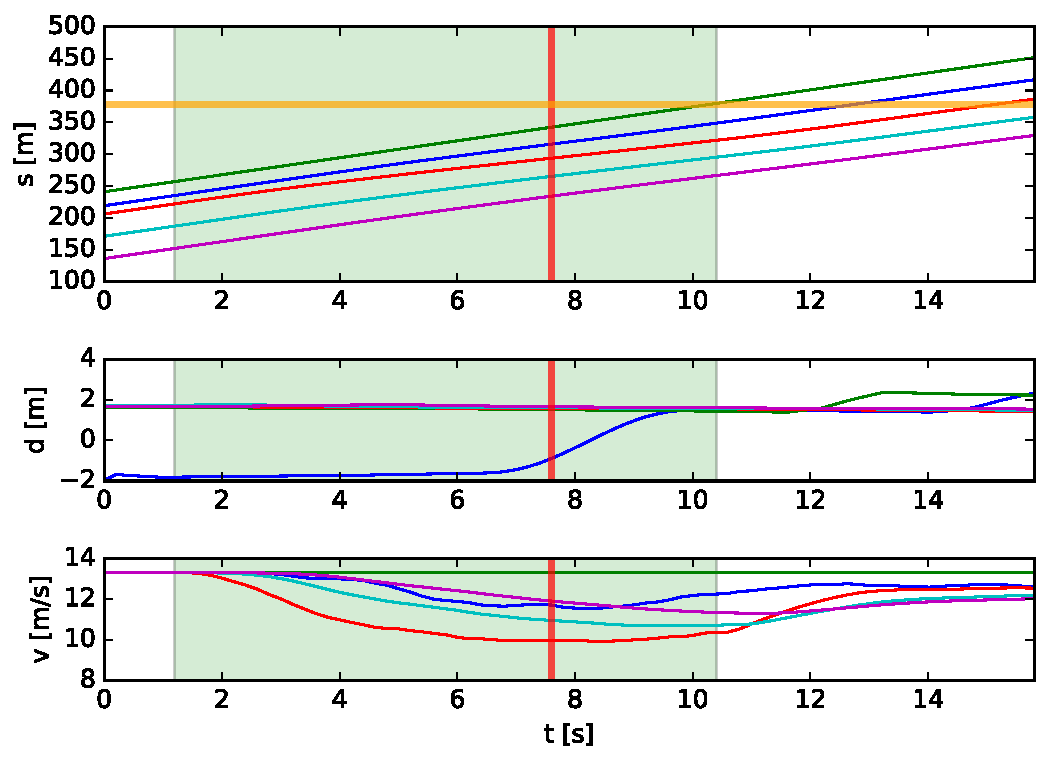
\includegraphics[width = 0.85 \textwidth ]{four_veh_results.pdf}
    \caption[Ergebnisse Szenario 2.1]{Kooperativer Fahrstreifenwechsel bei vier Fahrzeugen auf dem Zielfahrstreifen. F\"ur die Legende sei auf Abbildung~\ref{zweiFahrzeugeEgo} verwiesen.}
    \label{fig:VierFahrzeuge} 
\end{figure}


In den Abbildung~\ref{fig:VerschiedeneGeschwindigkeiten} sind die Simulationsergebnisse f\"ur verschiedene Anfangsgeschwindigkeiten des Ego"=Fahrzeuges zu sehen.
In Abbildung~\ref{40kmh} ist zu sehen, dass das Ego-Fahrzeug bei einer Anfangsgeschwindigkeit von 40 km/h die gleiche L\"ucke w\"ahlt wie in den zuvor betrachteten Szenarien.
In der ersten Sekunde folgt das Ego"=Fahrzeug noch der Trajektorie aus dem angenommenen vorausgegangen Zeitschritt.
Anschlie{\ss}end beschleunigt es und passt damit seine Geschwindigkeit den Fahrzeugen auf dem Zielfahrstreifen an.
Das zweite Fahrzeug auf dem Zielfahrstreifen (Fahrzeug 3) zeigt erneut ein kooperatives Verhalten und verringert seine Geschwindigkeit.
Damit wird der longitudinale Abstand zwischen den Fahrzeugen bis zum Fahrstreifenwechsel vergr\"o{\ss}ert, sodass sich eine L\"ucke bildet die gro{\ss} genug f\"ur einen sicheren Fahrstreifenwechsel des Ego"=Fahrzeuges ist.

In Szenario 2.3 startet das Ego"=Fahrzeug mit 30 km/h (siehe Abbildung~\ref{30kmh}).
Es besteht nicht mehr auf die L\"ucke zwischen den Fahrzeugen 2 und 3.
Wie in Szenario 2.2 beschleunigt das Ego"=Fahrzeug, um sich der Geschwindigkeit auf dem Zielfahrstreifen anzupassen.
Es beh\"alt jedoch eine deutlich geringere Geschwindigkeit bei bis das Fahrzeug 3 passiert ist.
Anschlie{\ss}end beschleunigt es erneut um sich der Optimalgeschwindigkeit anzun\"ahern.
In diesem Fall zeigt Fahrzeug 4 ein kooperatives Verhalten, indem es seine Geschwindigkeit verringert.
In Abbildung~\ref{25kmh} ist das Verhalten des Ego"=Fahrzeuges bei einer Startgeschwindigkeit von 25 km/h zu sehen.
Da sich hinter den vier Fahrzeugen auf dem Zielfahrstreifen eine L\"ucke ergibt, die gro{\ss} genug ist, beh\"alt das Ego"=Fahrzeug seine vergleichsweise niedrige Geschwindigkeit bei und l\"asst die Fahrzeuge auf dem Zielfahrstreifen passieren.
Es zwingt dadurch keines der Fahrzeuge auf dem Zielfahrstreifen dazu, seine Geschwindigkeit drastisch anzupassen.
Der Fahrstreifenwechsel findet ohne kooperatives Verhalten der Fahrzeuge auf dem Zielfahrstreifen statt.

Die Szenarien zeigen, dass der Ansatz durch die Annahme eines kooperativen Verhaltens der Fahrzeuge auf dem Zielfahrstreifen auch einen Fahrstreifenwechsel bei dichtem Verkehr erlaubt.
Ist die anf\"angliche Geschwindigkeit des Ego-Fahrzeuges niedriger als die der Fahrzeuge auf dem Zielfahrstreifen beschleunigt es zuerst, um seine Geschwindigkeit anzupassen und ordnet sich dann im Zielfahrstreifen ein.
Dieses Verhalten entspricht dem Verhalten, das auf einer Beschleunigungsspur gefordert ist.
Es kann jedoch auch gezeigt werden, dass das Ego"=Fahrzeug nicht auf ein kooperatives Verhalten der Fahrzeuge auf dem Zielfahrstreifen besteht, wodurch es selbst ein egoistisches Verhalten zeigen w\"urde.
Sind die eigenen Vorteile im Vergleich zu den Nachteilen der kooperativen Fahrzeuge nicht gro{\ss} genug wird nicht von einem kooperativen Verhalten der anderen Fahrzeuge ausgegangen.


\begin{figure}[!htbp]
    \centering
    \label{fig:VerschiedeneGeschwindigkeiten}
    \subfigure[40 km/h ]{
        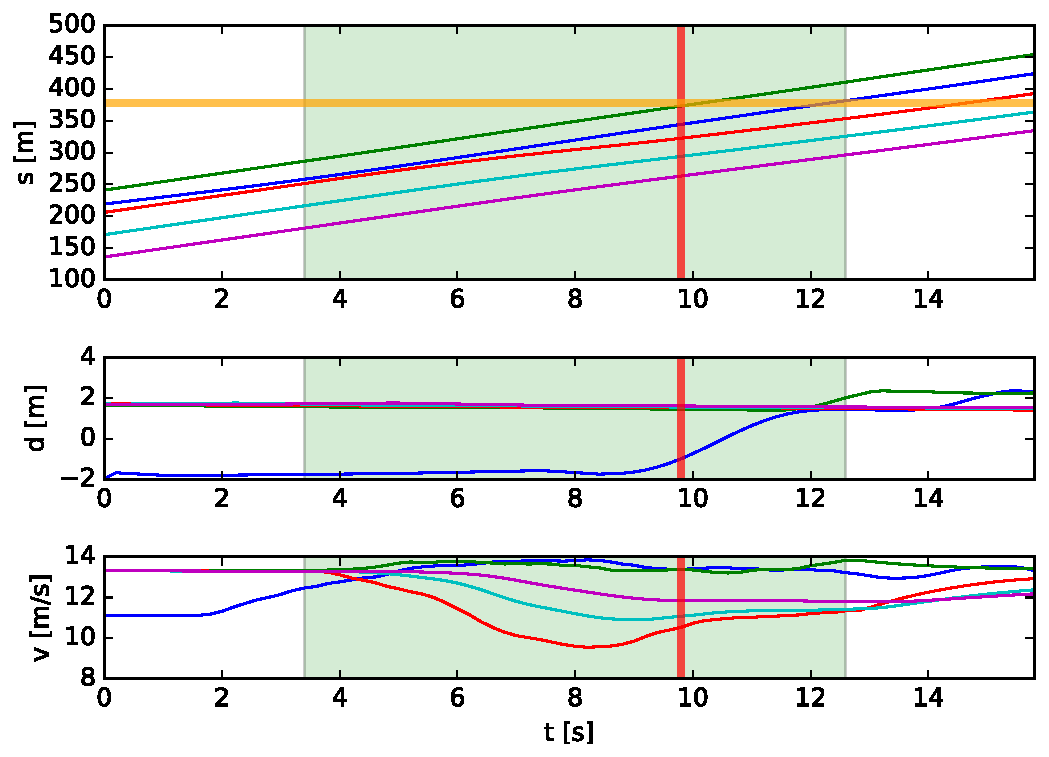
\includegraphics[width =  0.63 \textwidth]{40_kmh.pdf}
        \label{40kmh}
    }
    \subfigure[30 km/h]{
        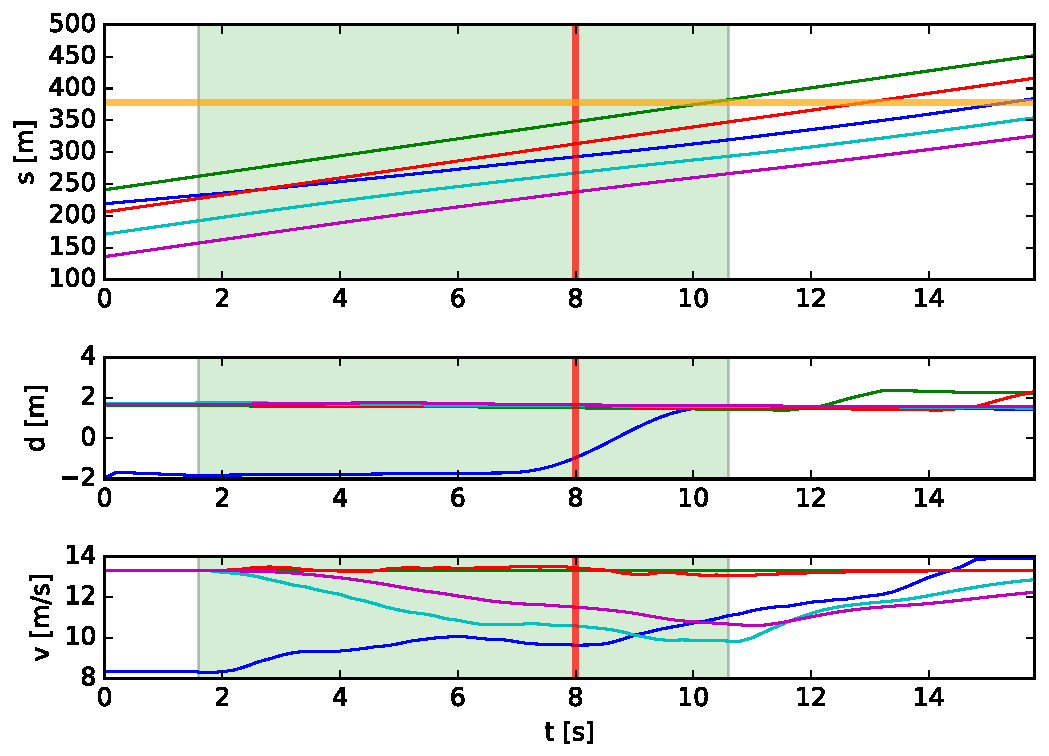
\includegraphics[width =  0.63 \textwidth]{30_kmh.pdf}
        \label{30kmh}
    }
    \subfigure[25 km/h]{
        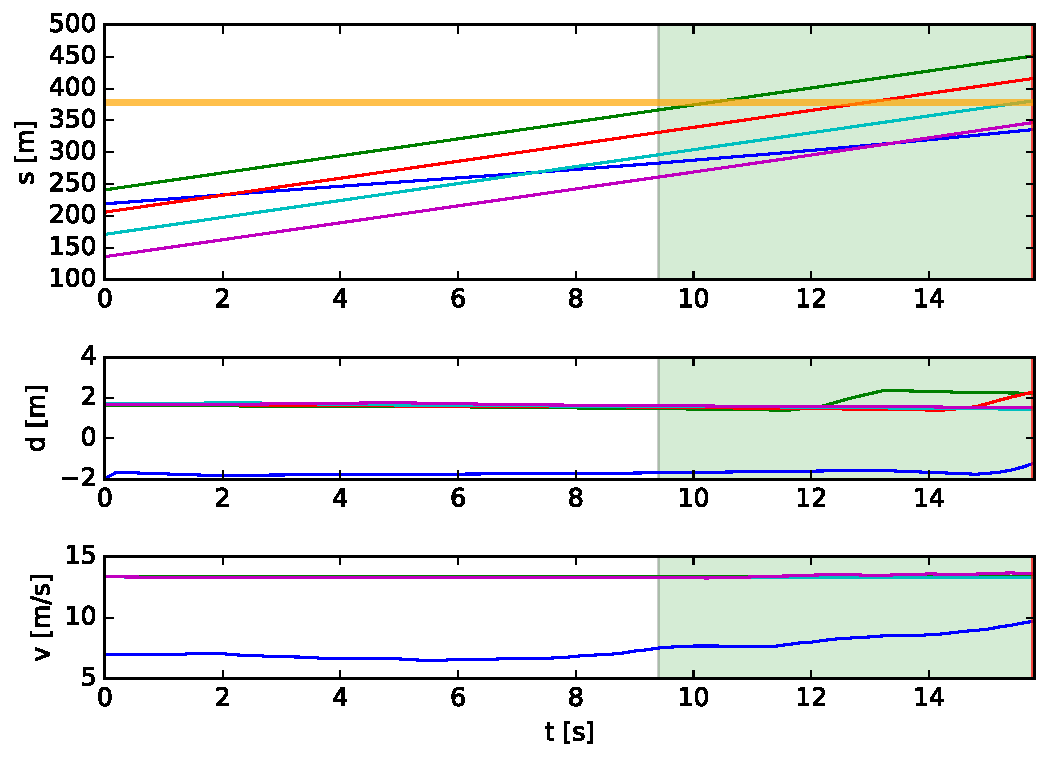
\includegraphics[width =  0.63 \textwidth]{25_kmh.pdf}
        \label{25kmh}
    }
    \caption[Verschiedene Anfangsgeschwindigkeiten]{Fahrstreifenwechsel bei verschiedenen Anfangsgeschwindigkeiten des Ego"=Fahrzeuges. F\"ur die Legende sei auf Abbildung~\ref{zweiFahrzeugeEgo} verwiesen.}
\end{figure}




\subsection{Fortlaufende Neuplanung}
\label{sec:AuswertungNauplanung}
In Kapitel~\ref{sec:einzelPlanungsschritt} konnte gezeigt werden, dass durch den vorgestellten Ansatz bei einem einzelnen Planungsschritt eine kooperative L\"osung gefunden werden kann.
Dabei wird ein kooperatives Verhalten der anderen Verkehrsteilnehmer angenommen.
Es soll nun \"uberpr\"uft werden, ob der Ansatz auch bei einer fortlaufenden Neuplanung zu einer sicheren, komfortablen und kooperativen Fahrstreifenwechseltrajektorie f\"uhrt.
Dazu wird zuerst von einem kooperativen Verhalten der anderen Verkehrsteilnehmer ausgegangen.
Anschlie{\ss}end wird \"uberpr\"uft zu welchem Ergebnis ein egoistisches Verhalten der anderen Verkehrsteilnehmer f\"uhrt.
Hierf\"ur wurde erneut ein Szenario mit zwei Fahrzeugen auf dem Zielfahrstreifen gew\"ahlt (siehe Abbildung~\ref{fig:two_veh_scene}).
Es wird angenommen, dass ein Planungsschritt in einer Zeit kleiner als \gls{symb:t_verarb} berechnet werden kann. 
Vom aktuellen Zeitpunkt  \gls{symb:t_jetzt} bis zum Zeitpunkt \gls{symb:t_jetzt} + \gls{symb:t_verarb} folgt Ego"=Fahzeug exakt der Trajektorie aus dem vorherigen Zeitschritt.
Anschlie{\ss}end steht eine neue Trajektorie zur Verf\"ugung.
Zu Beginn jedes Planungsschrittes ist die aktuelle Position aller Fahrzeuge bekannt.
Die Planung wird nicht mehr ver\"andert, nachdem dieser eingeleitet wurde.

\minisec{Neuplanung bei kooperativem Verhalten}
Es wird zuerst davon ausgegangen, dass die Fahrzeuge auf dem Zielfahrstreifen ein kooperatives Verhalten zeigen.
Dazu wird das Ergebnis aus dem ersten Planungsschritt als Verhalten der Fahrzeuge auf dem Zielfahrstreifen angenommen.


Das Ergebnis der Simulation ist in Abbildung~\ref{Replan} dargestellt.
Es ist ein \"ahnliches Trajektorienset wie bei einem einzelnen Planungsschritt zu erkennen.
Das Ego"=Fahrzeug sch\"atzt das kooperative Verhalten der Fahrzeuge auf dem Zielfahrstreifen richtig ein und f\"ahrt in die L\"ucke zwischen den Fahrzeugen auf dem Zielfahrstreifen ein.
Da die L\"osung des Multi-Agenten-Optimierungsproblems durch den randomisierten L\"osungsansatz nur angen\"ahert wird entspricht das Verhalten der Fahrzeuge, au{\ss}er im ersten Planungsschritt, nie exakt der Bewegungspr\"adiktion des Ego"=Fahrzeuges.
Trotz dieser Abweichung wird von dem vorgestellten Ansatz eine Trajektorie generiert, bei der auf das kooperative Verhalten der anderen Verkehrsteilnehmer reagiert wird und diese Verhalten f\"ur eine Fahrstreifenwechsel genutzt wird.
Dies zeigt, dass der Ansatz zu einem kooperativen Ergebnis f\"uhrt, solange sich die anderen Fahrzeuge \"ahnlich zur Bewegungspr\"adiktion verhalten.
Eine Bildabfolge des kooeprativen Fahrstreifenwechsels bei fortraufender Neuplanung ist im Anhang im Abbildung~\ref{fig:abfolgecoop} zu sehen.


\minisec{Neuplanung bei egoistischem Verhalten}
Es soll abschlie{\ss}end \"uberpr\"uft werden, wie das Ego"=Fahrzeug bei einer fortlaufenden Neuplanung auf ein egoistisches Verhalten der anderen Verkehrsteilnehmer reagiert.
Daf\"ur wird angenommen, dass die Fahrzeuge auf dem Zielfahrstreifen mit einer konstanten Geschwindigkeit fahren.

Die Ergebnisse sind in Abbildung~\ref{Replan_ego} dargestellt.
Die entsprechende Bildabfolge ist im Anhang in Abbildung~\ref{fig:abfolgeego} zu sehen.
Es ist zu sehen, dass der Ansatz bei einem egoistischen Verhalten der Fahrzeuge auf dem Zielfahrstreifen zu einem unerw\"unschten Fahrverhalten des Ego"=Fahrzeuges f\"uhrt.
Das Ego"=Fahrzeug geht davon aus, dass die Fahrzeuge auf dem Zielfahrstreifen sich kooperativ verhalten und die L\"ucke zwischen ihnen vergr\"o{\ss}ern.
Es erkennt das egoistische Fahrverhalten nicht und reagiert somit nicht darauf.
Dadurch kommt es beim Auffahren auf den Zielfahrstreifen zur deutlichen Unterschreitung von Sicherheitsabst\"anden.
Jeder Planungsschritt f\"uhrt zu dem Ergebnis, dass ein kooperatives Verhalten der Fahrzeuge auf dem Zielfahrstreifen zu geringen Gesamtkosten f\"uhrt.
Dadurch geht das Ego"=Fahrzeug bis zum Schluss davon aus, dass die Fahrzeuge auf dem Zielfahrstreifen die L\"ucke vergr\"o{\ss}ern werden um ihm das Auffahren auf den Zielfahrstreifen zu erleichtern.
Es z\"ogert den Fahrstreifenwechsel solange heraus, bis es am Ende des aktuellen Fahrstreifens angekommen ist.
Ein Anhalten auf dem aktuellen Fahrstreifen w\"urde dann eine unrealistische Verz\"ogerung erfordern.
Die L\"osung des Optimierungsproblems ergibt deshalb, dass ein Fahrstreifenwechsel die geringsten Kosten verursacht, selbst wenn dabei die Sicherheitsabst\"ande deutlich unterschritten werden. 
Es zeigt sich, dass der kooperative Planungsansatz bei einem unerwarteten Verhalten der anderen Fahrzeuge an seine Grenzen kommt.
In Kapitel~\ref{sec:diskussion} wird darauf eingegangen, wie diesen Grenzen entgegengewirkt werden kann.

\begin{figure}[!htbp]
    \centering
    \subfigure[Fortlaufende Neuplanung bei kooperativem Verhalten der Fahrzeuge auf dem Zielfahrstreifen]{
        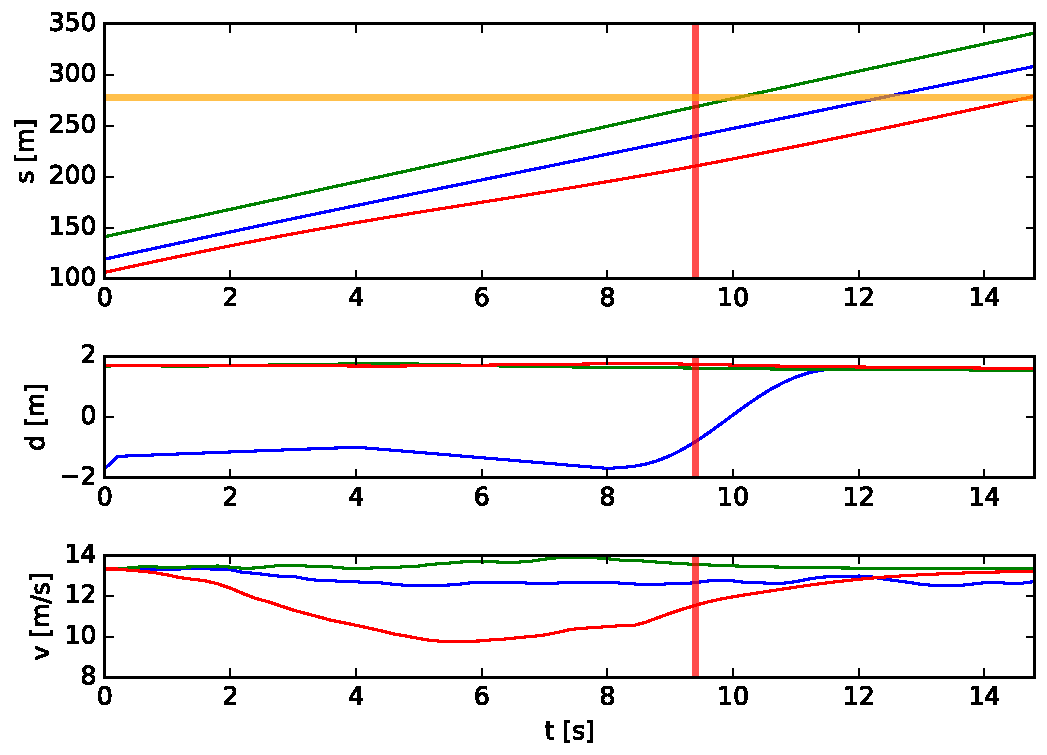
\includegraphics[width =  0.8 \textwidth]{Replan.pdf}
        \label{Replan}
    }
    \subfigure[Fortlaufende Neuplanung bei kooperativem Verhalten der Fahrzeuge auf dem Zielfahrstreifen]{
        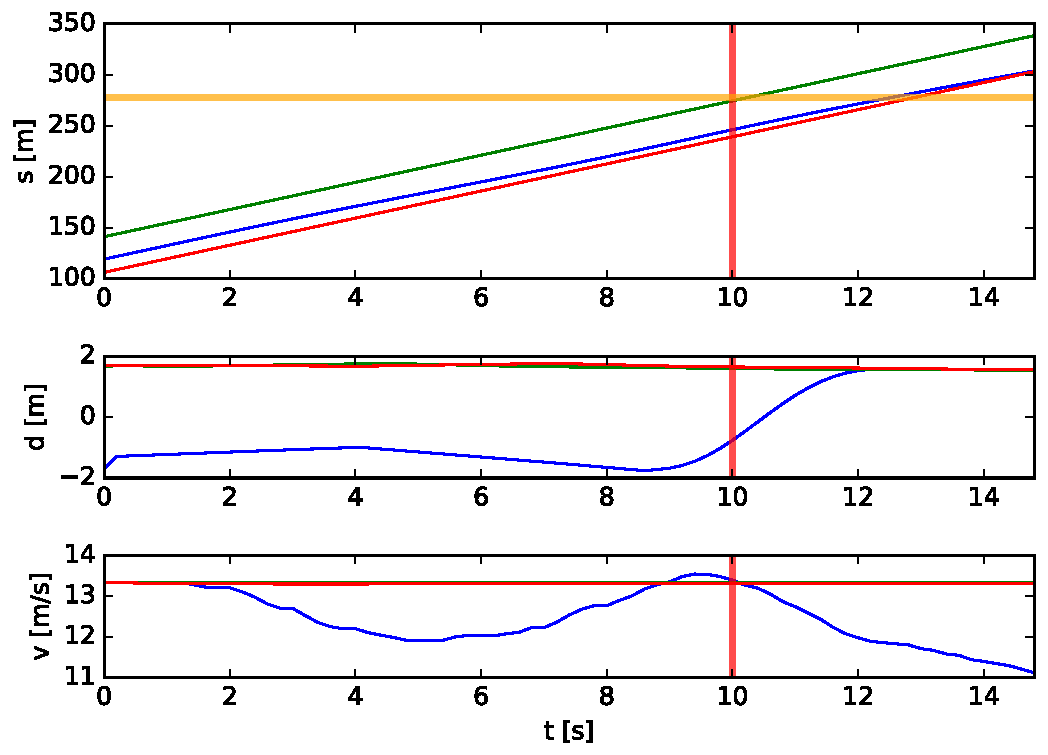
\includegraphics[width =  0.8 \textwidth]{Replan_ego.pdf}
        \label{Replan_ego}
    }
    \caption[Fortlaufende Neuplanung]{Fortlaufende Neuplanung. Die vertikale rote Line kennzeichnet den Zeitpunkt des Fahrstreifenwechsels \gls{symb:t_lc}.}
    \label{fig:Fort_Neuplanung}
\end{figure}




\section{Diskussion}
\label{sec:diskussion}
Es konnte gezeigt werden, dass der Ansatz zu einem Trajektorienset f\"uhrt, das einen kooperativen Fahrstreifenwechsel abbildet.
Es konnte auch gezeigt werden, dass der Ansatz zu einer sicheren und komfortablen Spruwechseltrajektorie f\"uhrt, solange sich die Fahrzeuge auf dem Zielfahrstreifen \"ahnlich zur Bewegungspr\"adiktion verhalten.
Das Verhalten des Ego"=Fahrzeuges und das erwartete Verhalten der anderen Verkehrsteilnehmer kann sich je nach Wahl der Parameter der Kostenfunktionale stark von einander unterscheiden.
Ob der Ansatz sich auch im realen Verkehr bew\"ahren kann h\"angt damit stark von den gew\"ahlten Parametern ab.

Das Kostenfunktional der anderen Fahrzeuge muss so bestimmt werden, dass es m\"oglichst gut ihr Verhalten widerspiegelt.
Da sich das Verhalten jedoch von Fahrer zu Fahrer unterscheidet, m\"usste auch das Kostenfunktional angepasst werden.
H\"aufig bleibt dem automatisierten Fahrsystem jedoch nur ein sehr kurze Zeitspanne um das Verhalten der Verkehrsteilnehmer zu beobachten.
Es ist nicht davon auszugehen, dass diese Zeit ausreicht um das Verhalten anderer Fahrzeuge zu analysieren und darauf beruhend ein angepasstes Kostenfunktional zu erstellen.

Eine M\"oglichkeit auf diesen Aspekt einzugehen ist, dass von einem allgemeinen Kostenfunktional ausgegangen wird.
Diese Kostenfunktional wird auf alle Fahrzeuge angewandt.
Es sollte deshalb m\"oglichst gut das allgemeine Fahrverhalten von nicht automatisierten Fahrzeugen repr\"asentieren.
Untersuchungen zur Generierung eines solchen Kostenfunktionals wurden von Tr\"unkle \cite{Trunkel} gemacht.
Da verschiedene Fahrsituationen ein unterschiedliches Verhalten fordern muss das Kostenfunktional noch entsprechend der Verkehrsregeln und der Ausgangssituation angepasst werden.
Verhalten sich die interagierenden Fahrzeuge \"ahnlich zu dem Fahrverhalten das durch das allgemeine Kostenfunktional ausgedr\"uckt wird, f\"uhrt der vorgestellte Planungsansatz zu einer kooperativen Fahrstreifenwechseltrajektorie.

In Kapitel~\ref{sec:AuswertungNauplanung} wurde jedoch auch gezeigt, dass der Ansatz an seine Grenzen ger\"at, sobald Fahrzeuge stark von dem angenommenen Verhalten abweichen.
Es wird deutlich, dass parallel zur kooperativen Planung weitere \"Uberpr\"ufungen stattfinden m\"ussen um auch bei unerwartetem Verhalten anderer Fahrzeuge ein sicheres Fahrverhalten zu garantieren.
In Naumann et al. \cite{Naumann2018} wird vorgeschlagen parallel zur kooperativen Planung eine \"Ubereinstimmungs\"uberpr\"ufung und eine Sicherheits\"uberpr\"ufung durchzuf\"uhren.
Bei der \"Ubereinstimmungs\"uberpr\"ufung wird abgesch\"atzt wie wahrscheinlich es ist, dass die anderen Fahrzeuge sich entsprechend der Bewegungspr\"adiktion verhalten.
Ergibt die \"Ubereinstimmungs\"uberpr\"ufung, dass sich ein Fahrzeug wahrscheinlich nicht kooperativ verhalten wird, kommt ein konservativer Ersatzplan zum Einsatz.
Bei einem Fahrstreifenwechsel w\"are ein konservativer Ersatzplan, dass das Fahrzeug auf dem aktuellen Fahrstreifen bleibt und seine Geschwindigkeit verringert.

In der Sicherheits\"uberpr\"ufung wird gepr\"uft ob sich das Fahrzeug in einem sicheren Zustand befindet.
Ist dies nicht der Fall wird ein Notfallplan durchgef\"uhrt.
Bei einem Fahrstreifenwechsel w\"are zu pr\"ufen ob zum Zeitpunkt des Fahrstreifenwechsels der Abstand zu den Fahrzeugen auf dem Zielfahrstreifen bereits gro{\ss} genug ist um einen sicheren Fahrstreifenwechsel zu garantieren.
Desweiteren sollte gepr\"uft werden bis zu welchem Zeitpunkt es noch m\"oglich ist mit einem sicheren Bremsman\"over bis zum Ende dem aktuellen Fahrstreifen zum Stehen zu kommen.
Ist zu diesem Zeitpunkt ein sicherer Fahrstreifenwechsel noch nicht garantiert sollte das entsprechende Bremsman\"over als Notfallplan ausgef\"uhrt werden.

In Kapitel~\ref{globaleLV} wurde darauf hingewiesen, dass ein randomisierter L\"osungsansatz der nach einer bestimmten Zeit oder Anzahl an Stichproben abgebrochen wird nicht zur exakten L\"osung f\"uhrt.
Damit wird nicht die optimale Trajektorie des Ego"=Fahrzeuges ermittelt, sondern in den meisten F\"allen eine Trajektorie die \"ahnlich zu der optimalen Trajektorie ist.
Da laut \cite{Naumann2018} auch menschliche Fahrer nicht strikte Optimalit\"at anstreben, sondern vielmehr eine Trajektorie die nahe am Optimum ist, kann durch den Ansatz auch bei leichten Abweichungen vom Optimum ein menschen\"ahnliches Fahrverhalten widergespiegelt werden.
Es ist auch darauf hinzuweisen, dass ein probabilistischer Ansatz bei zwei Planungsschritten gleicher Ausgangssituation zu stark unterschiedlichen L\"osungen f\"uhren kann wenn die beiden L\"osungen \"ahnliche Kosten verursachen.
In einem solchen Fall ist davon auszugehen, dass auch f\"ur menschliche Fahrer nicht eindeutig ist welche Strategie zu bevorzugen ist und gegebenenfalls eine L\"osung gew\"ahlt wird die nicht dem globalen Optimum entspricht.
Der Ansatz spiegelt deshalb auch in solchen F\"allen ein menschliches Verhalten wider, selbst wenn die Trajektorie stark von der Optimaltrajektorie abweicht.
Eine solche uneindeutige Situation wird gel\"ost, indem die beteiligten Fahrzeuge zun\"achst die Strategie w\"ahlen die ihnen besser erscheint.
Dabei ist es nicht wichtig, dass die gew\"ahlte Strategie der optimalen Strategie entspricht, solange sie zu \"ahnlichen Kosten f\"uhrt.
Anschlie{\ss}end wird auf die sich neu ergebende Situation reagiert und die Planung wiederholt, bis die zu w\"ahlende Strategie eindeutig ist.
Bei automatisierten Fahrzeugen wird dieses Verhalten durch die fortlaufende Neuplanung erzeugt.



% !TeX root = ../thesis.tex

\chapter{Zusammenfassung}
\label{sec:conclusion_future-work}
In dieser Arbeit wurde ein Trajektorienplanungsansatz f\"ur einen kooperativen Fahrstreifenwechsel vorgestellt.
In einer Multi"=Agenten"=Optimierung wird sowohl die Fahrstreifenwechseltrajektorie des Ego"=Fahrzeuges ermittelt als auch eine Bewegungspr\"adiktion der umgebenden Fahrzeuge erstellt.
Dadurch kann die Interaktion mit anderen Fahrzeugen abgebildet werden.
Das Optimierungsproblem wird durch ein randomisiertes Verfahren gel\"ost.
Daf\"ur werden zuf\"allige Trajektorien des Ego"=Fahrzeuges ermittelt und anschlie{\ss}end f\"ur jedes dieser Geschwindigkeitsprobleme ein Pfad generiert.
In einer inneren Optimierung wird f\"ur alle interagierenden Fahrzeuge eine kooperative Trajektorie ermittelt.
Alle andere Fahrzeuge verhalten sich entsprechend des \gls{idm}.
Die sich ergebenden Trajektoriensets werden durch ein Gesamtkostenfunktional bewertet, das neben den Kosten des Ego"=Fahrzeuges auch die Kosten der kooperativen Fahrzeuge ber\"ucksichtigt.

Der entwickelte Ansatz wird in verschiedenen Szenarien evaluiert.
Dabei wurden zun\"achst die Ergebnisse eines einzelnen Planungsschrittes untersucht.
Anschlie{\ss}end wurde das Verhalten des Ego"=Fahrzeuges bei einer fortlaufenden Neuplanung der Trajektorie betrachtet.
Dazu wurde zuerst von einem kooperativen und anschlie{\ss}end von einem egoistischen Verhalten der Fahrzeuge auf dem Zielfahrstreifen ausgegangen.


\section{Fazit}
Es konnte gezeigt werden, dass durch den vorgestellten Ansatz ein Trajektorienset mit einem kooperativen und sicheren Fahrstreifenwechsel erzeugt wird.
Die Kosten des Fahrstreifenwechsels, die anhand des vorgestellten Kostenfunktionals berechnet wurden, konnten im Vergleich zu einem unkooperativen Fahrstreifenwechsel deutlich herabgesetzt werden.
Auch bei dichtem Verkehr auf dem Zielfahrstreifen wird ein Trajektorienset generiert, bei dem das Ego"=Fahrzeug einen kooperativen Fahrstreifenwechsel vollzieht, ohne dabei auf dem aktuellen Fahrstreifen stehen bleiben zu m\"ussen.

Es konnte weiterhin gezeigt werden, dass das Ego"=Fahrzeug nicht nur von einem kooperativen Fahrverhalten der anderen Teilnehmer ausgeht sondern selbst auch ein kooperatives Fahrverhalten beim Fahrstreifenwechsel zeigt.
Sind aufgrund einer niedrigeren Anfangsgeschwindigkeit des Ego"=Fahrzeuges die Nachteile der Fahrzeuge auf dem Zielfahrstreifen im Vergleich zu den eigenen Vorteilen zu hoch, wird eine L\"ucke gew\"ahlt die nicht zur Minimierung des eigenen Kostenfunktionals f\"uhrt.
Damit wird ein starkes Ausbremsen der Fahrzeuge auf dem Zielfahrstreifen vermieden, solange eine andere L\"ucke in Aussicht ist, die f\"ur den Fahrstreifenwechsel genutzt werden kann.

Bei einer fortlaufenden Neuplanung f\"uhrt der vorgestellte Ansatz ebenfalls zu einer kooperativen und sicheren Fahrstreifenwechseltrajektorie solang sich die anderen Fahrzeuge \"ahnlich zur in der Optimierung generierten Bewegungspr\"aditkion verhalten.
Es wurde jedoch auch ersichtlich, dass der Ansatz zu einem unerw\"unschten Fahrverhalten des Ego"=Fahrzeuges f\"uhrt wenn die anderen Fahrzeuge stark von der Bewegungspr\"adiktion abweichen und sich egoistisch verhalten.
Um einen sicheren Fahrstreifenwechsel garantieren zu k\"onnen muss der vorgestellte Ansatz deshalb durch parallel dazu laufende Sicherheits\"uberpr\"ufungen erg\"anzt werden.

Der vorgestellte Ansatz wurde in Szenarien mit unterschiedlich vielen Fahrzeugen auf dem Zielfahrstreifen simuliert.
Dabei konnte gezeigt werden, dass die Laufzeit weniger als linear mit der Anzahl der Fahrzeuge zunimmt.



\section{Ausblick}
Ziel des Trajektorienplanungsansatzes ist die Anwendung im realen Verkehr.
Um dies zu erreichen muss der Planungsalgorithmus echtzeitf\"ahig sein, eine sichere Fahrstreifenwechseltrajektorie garantieren und es m\"ussen getroffene Annahmen aufgehoben bzw. aufgelockert werden.

Bei der derzeitigen Implementierung weicht die Laufzeit des Algorithmus stark von der Laufzeit ab, die f\"ur eine Echtzeitf\"ahigkeit gefordert w\"are.
Um dies zu erreichen sollte auf eine interpretierte Programmiersprache wie Python verzichtet werden und auf eine Programmiersprach zur\"uckgegriffen werden die ein effizientes ausf\"uhrendes Programm erzeugt (z.B. C++).
Ein hohes Potenzial um die Laufzeit des Algorithmus deutlich zu verringern birgt au{\ss}erdem, das innere Optimierungsproblem durch ein weitaus effizienteres lokales L\"osungsverfahren zu ersetzten.
In dem vorgestellten Ansatz wurde sowohl f\"ur die innere als auch f\"ur die \"au{\ss}ere Optimierung ein randomisiertes Verfahren genutzt.
Da in der inneren Optimierung bis auf die Trajektorie des betrachteten Fahrzeuges alle Trajektorien vorgegeben sind, ist hier unter zuhilfenahme von vereinfachenden Annahmen ein lokales L\"osungsverfahren vorstellbar.

Um trotz eines kooperativen Planungsansatzes die Sicherheit beim Fahrstreifenwechsel zu garantieren m\"ussen weitere \"Uberpr\"ufungen parallel zum Planungsalgorithmus durchgef\"uhrt werden.
Diese \"Uberpr\"ufungen m\"ussen garantieren, dass ein Fahrstreifenwechsel nur durchgef\"uhrt wird, wenn sichergestellt ist, dass der Fahrstreifenwechsel zu keinem Unfall f\"uhrt, f\"ur den das Ego"=Fahrzeuge verantwortlich gemacht werden kann.
Ziel einer zuk\"unftigen Arbeit k\"onnte die Erarbeitung eines Sicherheitskonzeptes f\"ur ein Fahrstreifenwechsel sein.
Dieses Sicherheitskonzept sollte sowohl verschiedene Sicherheits\"uberp\"ufungen, die f\"ur einen sicheren Fahrstreifenwechsel notwendig sind, beinhalten als auch entsprechende Notfallpl\"ane falls eine Sicherheitsbedingung verletzt wird.

In dieser Arbeit wurden Annahmen getroffen, die die Anwendung des Planungsansatzes auf spezielle Szenarien beschr\"ankt.
Unter anderem wurde davon ausgegangen, dass kein anderes Fahrzeug w\"ahrend des Planungshorizontes einen Fahrstreifenwechsel vornimmt.
Damit war der Pfad der anderen Fahrzeuge vorgegeben und es konnte auf eine einfache fahrstreifenbasierte Pr\"adiktion zur\"uckgegriffen werden.
Haben mehrere Fahrzeuge eine Fahrstreifenwechselintension wird die Fahrsituation erheblich komplexer.
Es m\"ussen nun auch Fahrstreifenwechselinteraktionen, an denen das Ego"=Fahrzeug nicht beteiligt ist, ber\"ucksichtig werden.
Kommt es zur Interaktion mit einem Fahrzeug das ebenfalls eine Fahrstreifenwechselintenstion hat, muss in der Optimierung nicht nur ein kooperatives Geschwindigkeitsprofil des anderen Fahrzeuges erzeugt werden sondern auch der entsprechende Pfad.
In einer zuk\"unftigen Arbeit k\"onnte der bestehende Ansatz entsprechend erweitert werden und somit eine Vielzahl verschiedener Fahrstreifenwechselszenarien abgedeckt werden.      


% ----------------------------------------------------------------------------------------------
%|                                    Appendix + Glosseries                                     |
% ----------------------------------------------------------------------------------------------
\appendix
\chapter{Anhang}
\label{appendix}

\section{Evaluationsparameter}
\label{sec:eval_param}



\sisetup{round-mode = places, round-precision = 2, scientific-notation = fixed, fixed-exponent = 0}
\begin{table}[!htbp]
    \centering
    \begin{tabular}{crSSSS}
        \hline
        & Anzahl an Samplen \(n\)& \( 1000\)\\
        & {Diskretisierung Schrittweite \gls{symb:h}} & \(0.2 \mathrm{s}\)\\
        & Planungshorizont \(t_\mathrm{planhozion}\)& \(15 \mathrm{s}\)\\
        & Nauplanungsintervall \gls{symb:t_verarb} & \(1\mathrm{s}\) \\
        & Fahrstreifenwechseldauer \gls{symb:t_lcd} & \(4\mathrm{s}\) \\
        & Gew\"unschter Zeitsabstand \gls{symb:t_abs} & \(1.8\mathrm{s}\) \\
        & Grenzverz\"ogerung \gls{symb:b_krit} & \(1.5\mathrm{m/s^2}\) \\   
        & Angenommen Beschleunigung nach Kooperation \gls{symb:a_lcend} & \(0.5\mathrm{m/s^2}\) \\           
         \hline
    \end{tabular}
    \caption[Simulations Parameter]{Simulations Parameter
    }\label{tab:Simpara}
\end{table}


\sisetup{round-mode = places, round-precision = 2, scientific-notation = fixed, fixed-exponent = 0}
\begin{table}[!htbp]
    \centering
    \begin{tabular}{crSSSS}
        \hline
        & & \(a\)  [m/s\textasciicircum 2] & \( v\) [km/h] & \(d_{normal}\) [m] \\%
        \hline
         & \gls{symb:f_opt} & 00.00e+00 & 48.00e+00 & 1.1e+00\\
         & \gls{symb:f_discstartp} & 1.50e+00 & 58.00e+00 & x \\
         & \gls{symb:f_discstartn} & -1.50e+00 & 33.00e+00 & 1.00e+00\\
         & \gls{symb:f_infstartp} & 5.00e+00 & x & x \\
         & \gls{symb:f_infstartn} & -7.50e+00 & 0.00e+00 & 0.1e+00\\
          \hline
    \end{tabular}
    \caption[Grenzwerte des Kostenfunktionals]{Grenzwerte des Kostenfunktionals. \gls{symb:f_opt} legt den Optimalwert fest. \gls{symb:f_discstartp} und \gls{symb:f_discstartn} den Beginn der Diskomfortzonen und \gls{symb:f_infstartp} und \gls{symb:f_infstartn} den Beginn der Unrealisierbarkeitszone
    }\label{tab:Kostfunc}
\end{table}



\sisetup{round-mode = places, round-precision = 2, scientific-notation = fixed, fixed-exponent = 0}
\begin{table}[!htbp]
    \centering
    \begin{tabular}{crSSSS}
        \hline
        & Wunschgeschwindigkeit \( v_{0} \) & \( 48  \mathrm{\frac{km}{h}}\)\\
        & Minimalabstand \(s_{0}\) & \(2\mathrm{m}\)\\
        & Gew\"unschte Zeitl\"ucke \( T \) & \(1.5\mathrm{s}\) \\
        & Maximale Beschleunigung \( a \) & \(2\mathrm{\frac{m}{s^2}}\) \\
        & Komfortable Verz\"ogerung \( b \) & \(2\mathrm{\frac{m}{s^2}}\) \\
        & Beschleunigungsexponent \( \delta \) & \(4\)\\
        
         \hline
    \end{tabular}
    \caption[IDM Parameter]{\gls{idm} Parameter
    }\label{tab:IDMpara}
\end{table}


\section{Bildabfolgen}
\label{sec:bildabfolge}

\begin{figure}[!htbp]
    \centering
    \label{fig:abfolgecoop}
    \subfigure[t = 1s ]{
        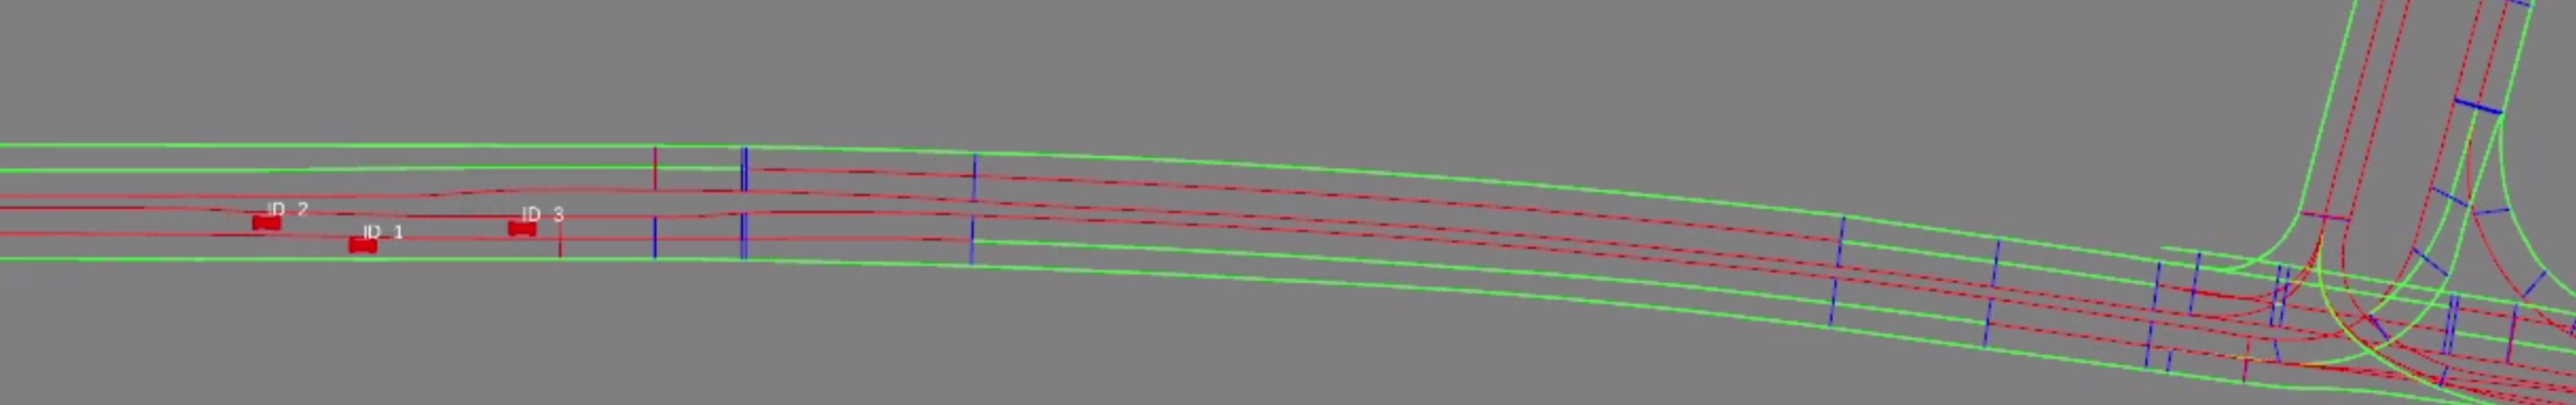
\includegraphics[width =  0.9 \textwidth]{coopt_1.pdf}
    }
    \subfigure[t = 3s ]{
        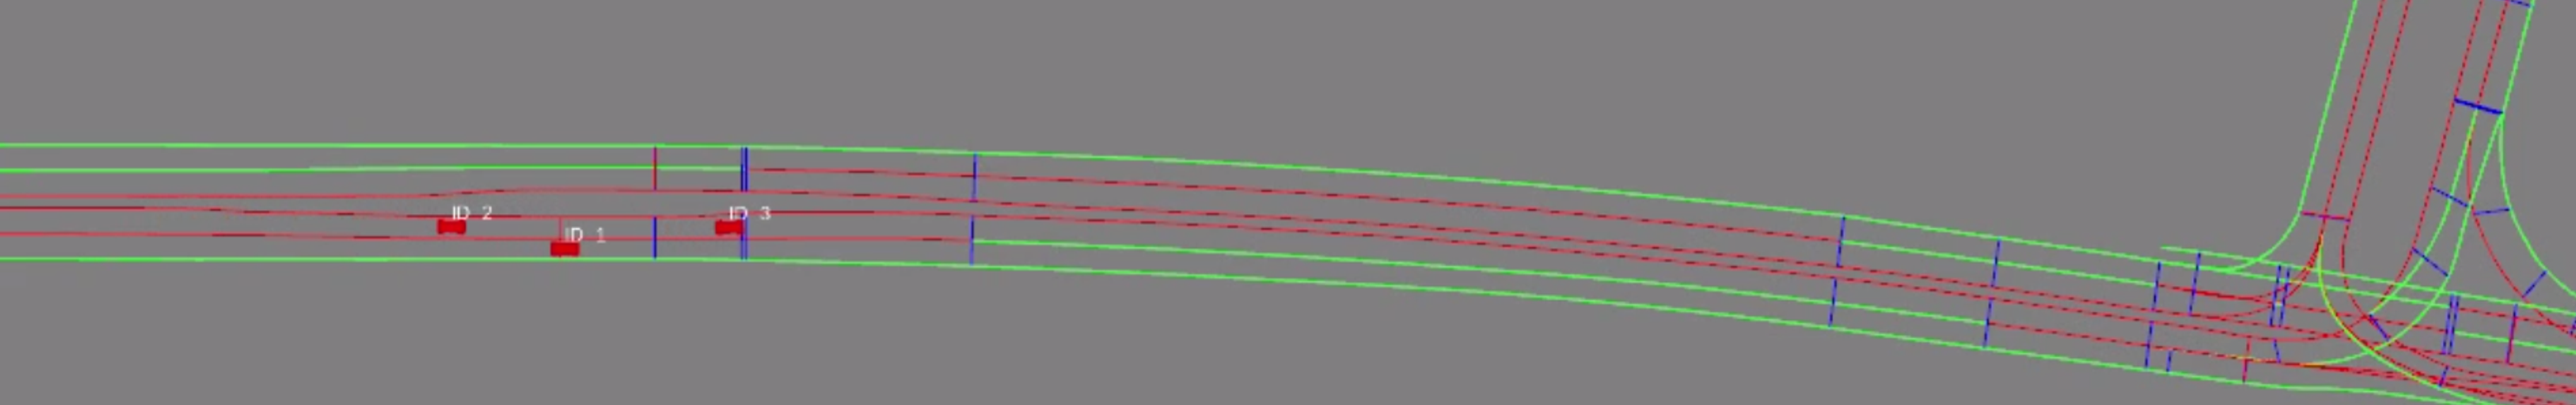
\includegraphics[width =  0.9 \textwidth]{coopt_3.pdf}
    }
    \subfigure[t = 5s ]{
        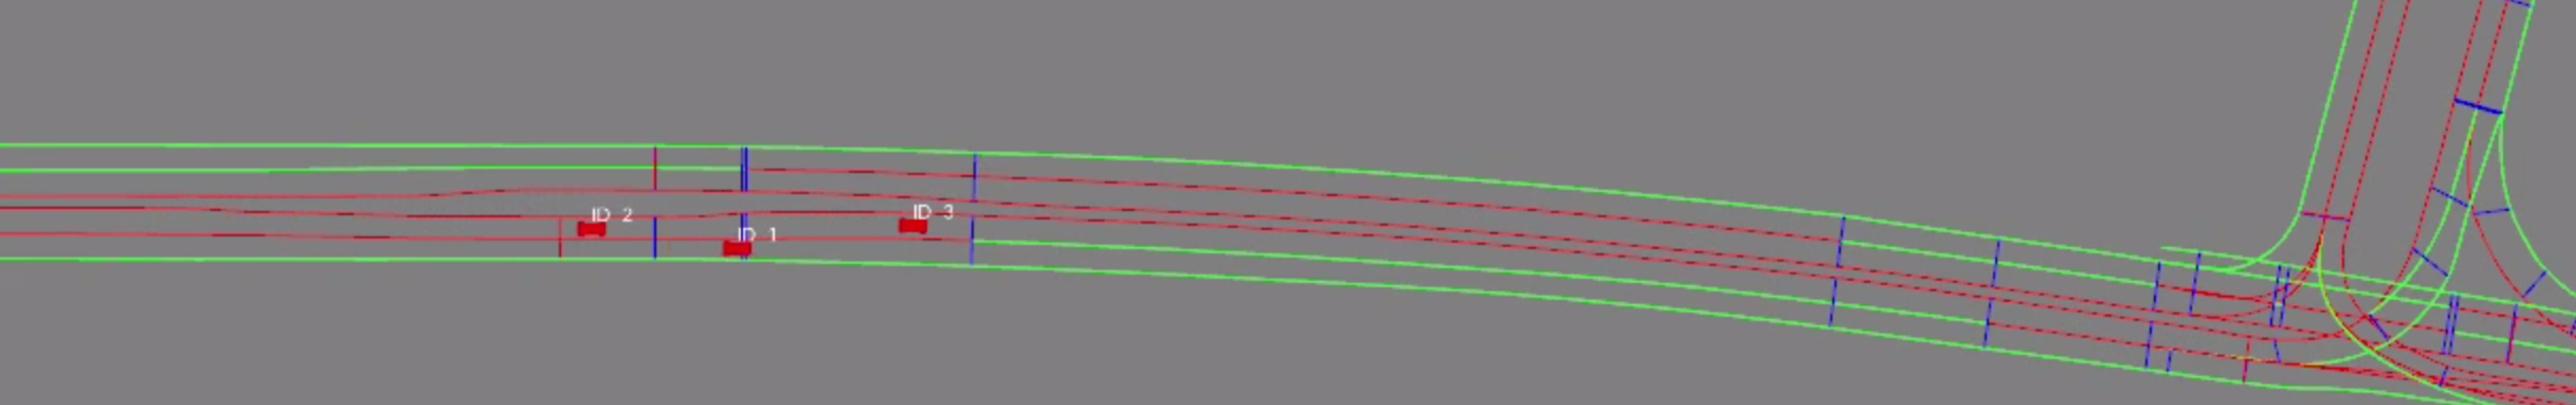
\includegraphics[width =  0.9 \textwidth]{coopt_5.pdf}
    }
    \subfigure[t = 7s ]{
        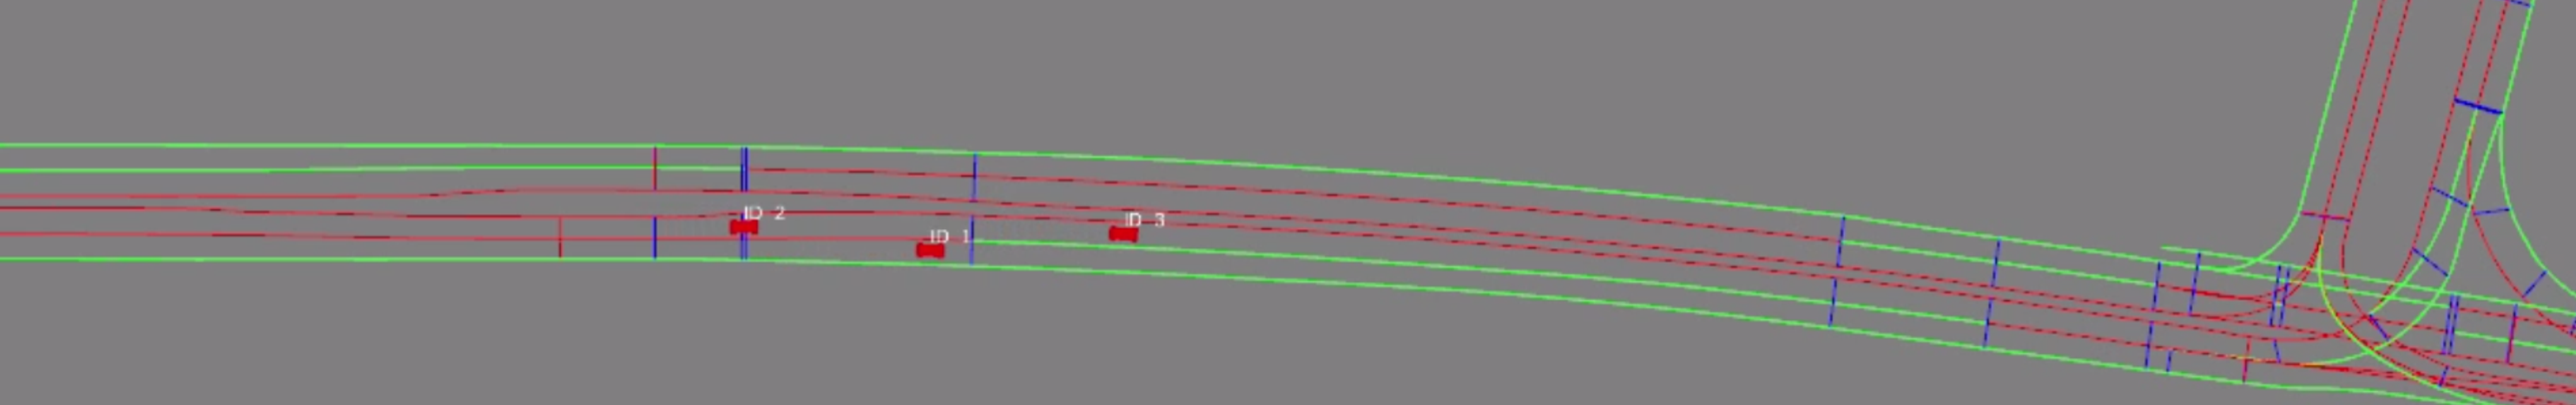
\includegraphics[width =  0.9 \textwidth]{coopt_7.pdf}
    }
    \subfigure[t = 9s ]{
        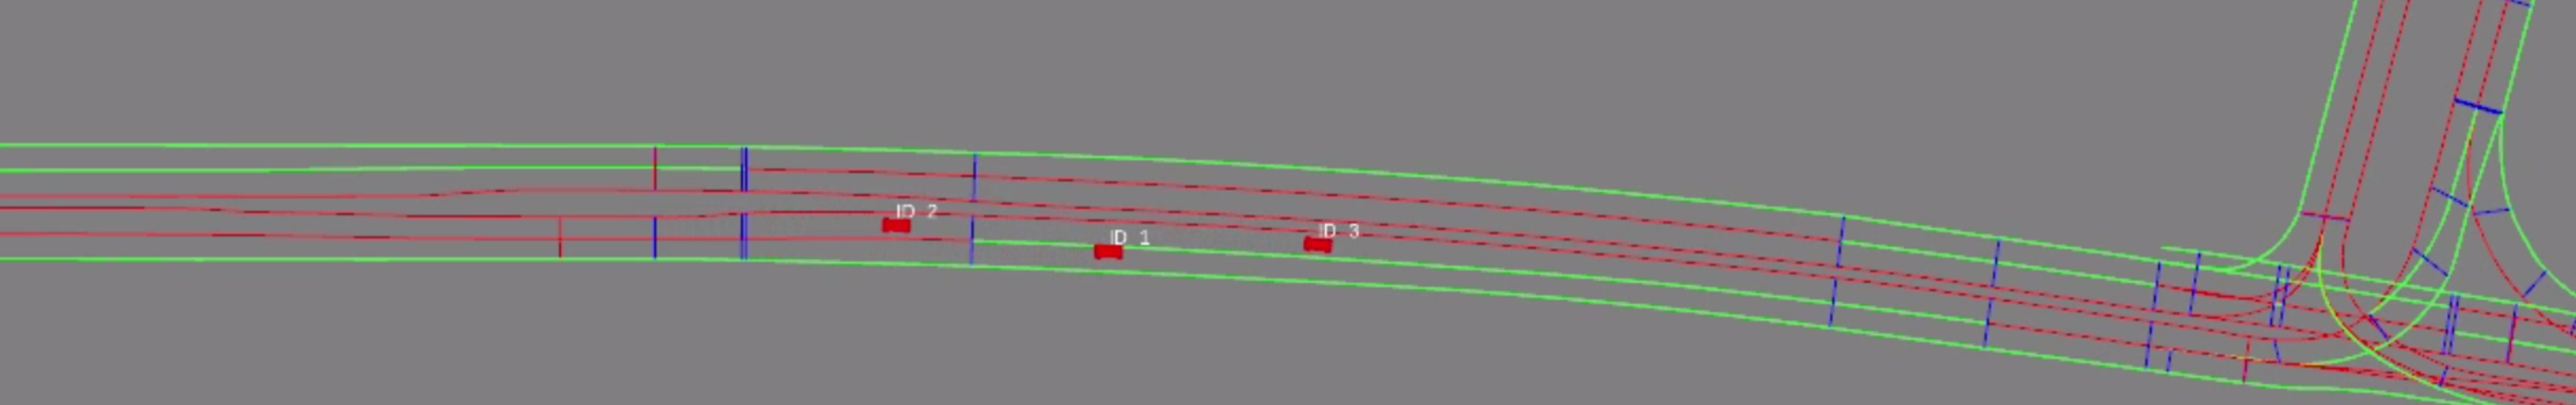
\includegraphics[width =  0.9 \textwidth]{coopt_9.pdf}
    }
    \subfigure[t = 11s ]{
        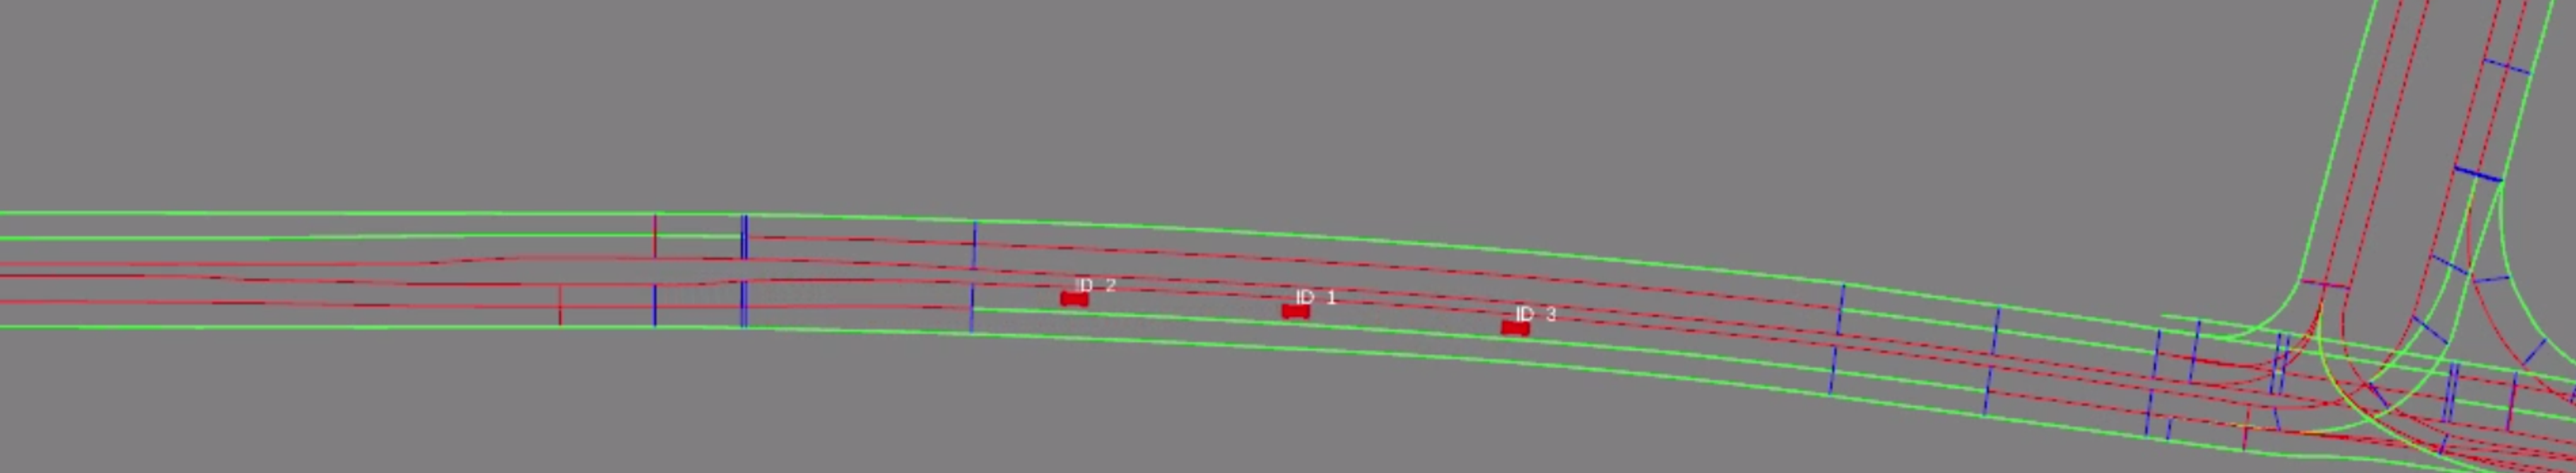
\includegraphics[width =  0.9 \textwidth]{coopt_11.pdf}
    }
    \subfigure[t = 13s ]{
        \includegraphics[width =  0.9 \textwidth]{coopt_13.pdf}
    }
    \caption[Bildabfolge kooperativ]{Bildabfolge eines kooperativen Fahrstreifenwechsels bei sek\"undlicher Neuplanung}
\end{figure}


\begin{figure}[!htbp]
    \centering
    \label{fig:abfolgeego}
    \subfigure[t = 1s ]{
        \includegraphics[width =  0.9 \textwidth]{egot_1.pdf}
    }
    \subfigure[t = 3s ]{
        \includegraphics[width =  0.9 \textwidth]{egot_3.pdf}
    }
    \subfigure[t = 5s ]{
        \includegraphics[width =  0.9 \textwidth]{egot_5.pdf}
    }
    \subfigure[t = 7s ]{
        \includegraphics[width =  0.9 \textwidth]{egot_7.pdf}
    }
    \subfigure[t = 9s ]{
        \includegraphics[width =  0.9 \textwidth]{egot_9.pdf}
    }
    \subfigure[t = 11s ]{
        \includegraphics[width =  0.9 \textwidth]{egot_11.pdf}
    }
    \subfigure[t = 13s ]{
        \includegraphics[width =  0.9 \textwidth]{egot_13.pdf}
    }
    \caption[Bildabfolge kooperativ]{Bildabfolge eines unkooperativen Fahrstreifenwechsels bei sek\"undlicher Neuplanung, bei dem das Ego"=Fahrzeug von einem kooperativen Verhalten ausgeht}
\end{figure}


\newpage
%--------------------------------------------------------------------------------


% List of Figures
\cleardoublepage
\addcontentsline{toc}{chapter}{\listfigurename}
\listoffigures

% Liste of Tables
\cleardoublepage
\addcontentsline{toc}{chapter}{\listtablename}
\listoftables

% Bibliography
\bibliographystyle{IEEEtranSA}   		                                        % IEEE Alphanumeric
\cleardoublepage
\addcontentsline{toc}{chapter}{Literaturverzeichnis}
\bibliography{thesis_bibtex}

% Online References
\ifuseglossaries
	\printglossary[type=onlineref, style=mylist]
\else
\fi


\end{document}
